\documentclass[12pt,a4paper,twoside,openright]{report}
\usepackage{preamble} % imported packages/macros/styling

% for commenting
\usepackage{xcolor}
\newcommand\az[1]{\textcolor{blue}{{\bf [AZ:} #1{\bf]}}}

\usepackage[sorting=none]{biblatex}
\addbibresource{ref.bib}

\begin{document}
% ----------------------------------------------------------------------
%TC:ignore
% title page
\pagestyle{empty}

\rightline{\LARGE \textbf{Yulin(Kyra) Zhou}}

\vspace*{60mm}
\begin{center}
	\Huge
	\textbf{Backdoor Attacks On \\ NLP Prompting} \\[3mm]
	\begin{figure}[!h]
        \centering
    
\includegraphics[width=0.4\textwidth]{figures/university_shield.png}
\end{figure}
    \huge
	Computer Science Tripos -- Part II \\[4mm]
    Queens' College \\[4mm]
	\today \\ [4mm]
\end{center}

% \today \\ [95mm]

\thispagestyle{empty}

% ----------------------------------------------------------------------

\pagestyle{plain}

\pagenumbering{roman}
\setcounter{page}{1}
\newpage
% declaration of originality
\section*{Declaration}

 {
  \setlength{\parskip}{\bigskipamount}

  I, Yulin(Kyra) Zhou of Queens' College, being a candidate for Part II of the Computer Science Tripos, hereby declare that this dissertation and the work described in it are my own work, unaided except as may be specified below, and that the dissertation does not contain material that has already been used to any substantial extent for a comparable purpose. In preparation of this dissertation I did not use text from AI-assisted platforms generating natural language answers to user queries, including but not limited to ChatGPT.

  I, Yulin(Kyra) Zhou of Queens' College, am content for my dissertation to be
  made available to the students and staff of the University.

  \emph{Signed:} Yulin(Kyra) Zhou

  \setlength{\parskip}{\smallskipamount}

  \emph{Date:} \today
 }

% Acknowledgements
\section*{Acknowledgements}

I sincerely appreciate the invaluable guidance my supervisors, Aaron Zhao, Ilia Shumailov, and Robert Mullins, provided throughout the project. I am also grateful to Wenyang Zhou, Yuang Chen, and Will Yu for their constructive comments on this dissertation. Finally, I sincerely thank Ramsey Faragher, Alastair Beresford, and Andy Rice, my Director of Studies, for their generous support over the past three years.

% proforma
\chapter*{Proforma}
 {\large
  \begin{tabular}{ll}
	  Candidate number:   & \bf 2365G                                      \\
	  Project Title:      & \bf Backdoor Attacks On NLP Prompting        \\
	  Examination:        & \bf Computer Science Tripos -- Part II, 2023 \\
	  Word Count:         & \bf 12000\footnotemark[1]                     \\
	  Code Line Count:    & \bf 5844\footnotemark[2]                     \\
	  Project Originator: & \bf Aaron Zhao                  \\
	  Project Supervisor: & \bf Aaron Zhao                       \\
	  Project Co-supervisor: & \bf Ilia Shumailov, Robert Mullins \\
  \end{tabular}
 }
\footnotetext[1]{This word count was computed using \texttt{texcount (https://app.uio.no/ifi/texcount/)}. Tables are included using \texttt{\%TC:group tabular 1 1} and \texttt{\%TC:group table 0 1}.}
\footnotetext[2]{This code line count was computed using \texttt{cloc (https://cloc.sourceforge.net/)}.}
\stepcounter{footnote}

\section*{Original Aims of the Project}
In natural language processing, Pre-trained Language Models (PLM) based on deep neural networks are commonly fine-tuned for end-user tasks. However, limited training data poses a challenge for achieving high performance using this \emph{pre-train then fine-tune} approach. Prompt-based learning is a new paradigm that directly probes knowledge from the PLM without extensive fine-tuning to overcome this limitation. Nevertheless, advances in prompt-based learning raise security concerns, such as backdoor attacks, in which attackers create hidden model behaviour that specific input patterns can trigger. This project compares the performance of different prompting models and assesses their vulnerability to backdoor attacks with different settings.

\section*{Work Completed}
The project successfully fulfilled the proposed criteria and explored additional ideas triggered by experimental results. First, I developed an extensible and robust framework to re-implement and compare three published prompting models and investigated whether automated prompting outperforms manual prompting. Then I re-implemented a backdoor attack on the prompting models to exploit the vulnerabilities of the models. The project extended the literature by incorporating multiple backdoor attacks with different design choices and a visualisation toolkit to comprehend the factors contributing to the varied effectiveness of backdoor attacks on the prompting models.

\section*{Special Difficulties}

None.

% table of contents
\tableofcontents

% list of figures
% \listoffigures

% ----------------------------------------------------------------------
\newpage
\pagenumbering{arabic}
%TC:endignore
%TC:group table 0 1
%TC:group tabular 1 1
% main chapters
% allocate 2 page
\chapter{Introduction}
\section{Motivation}
\label{section:motivation}
Pre-trained language models (PLMs) are deep neural networks trained on vast corpora, such as Wikipedia, to predict a masked-out word or sentence given the context. These models have shown effectiveness in many natural language processing (NLP) applications \cite{Devlin18BERT}. The idea of \textit{pre-train then fine-tune} approach applies the knowledge of the PLM to new downstream end-user tasks. During training, an additional neural network layer is added on top of the PLM and parameters are fine-tuned using training samples of the downstream task. However, producing high-performing models with this \emph{pre-train then fine-tune} approach with limited training data is challenging. Prompt-based learning (PL) \cite{Liu21} is a new paradigm that achieved state-of-the-art performance on a range of NLP tasks, particularly under few-shot learning scenarios where only a few training samples are available.

\begin{figure}[!ht]
    \centering
    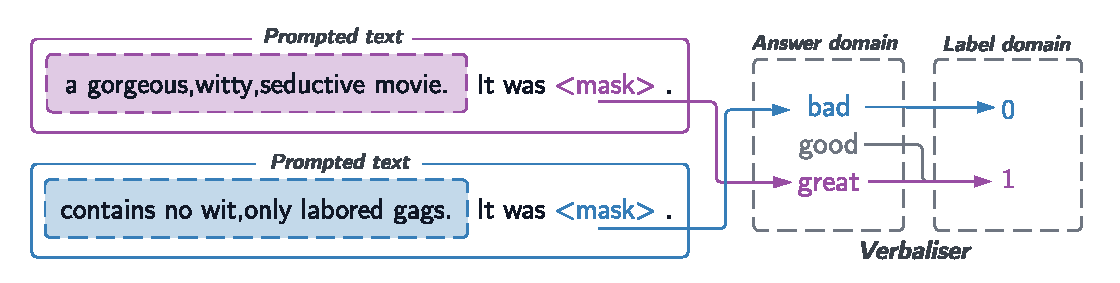
\includegraphics[width=\hsize]{figures/introduction_media/intro-pl.pdf}
    \caption{Prompt-based learning for sentiment analysis on movie reviews.}
    \label{fig:intro-pl}
\end{figure}

\vspace{-1.2em}
\paragraph{PL directly probes knowledge from PLMs} Instead of the \textit{pre-train then fine-tune} approach, PL modifies the input text, such as a movie review shown in \Cref{fig:intro-pl}, with a prompt. The prompt is a template with one or more placeholders called $<$\textit{mask}$>$ tokens. By asking the PLM to fill in the blanks, PL converts the problem into a cloze completion task. Additionally, PL incorporates a verbaliser that links candidate words (e.g., the word \textit{great}) to output labels (e.g., label \textit{1}). The verbaliser maps the optimal word the PLM selects to a label that serves as the final prediction. Without fine-tuning an extensive set of parameters, PL can more efficiently and explicitly use the knowledge in the PLM to fit the downstream task.

\vspace{-0.8em}
\paragraph{PL models are vulnerable} Advances in PL have brought the security vulnerabilities of the paradigm to the forefront. Recent research has investigated the possibilities of injecting backdoors into PLMs \cite{Lei22, Du22}. A backdoor-triggered attack can totally control or severely impact the performance of prompt-based models. By embedding backdoors into the PLM, it preserves normal model behaviour and only acts maliciously when the model encounters some pre-defined triggers in the input text. 

\vspace{1em}
This project aims to re-implement various prompt-based models, exploit their vulnerabilities under backdoor attacks and seeks to answer the following two questions:
\begin{itemize}[topsep=0pt, itemsep=0.8pt, partopsep=0pt]
    \item Under a few-shot scenario, whether one prompting model outperforms another, and why?
    \item To what extent is each prompting model robust under backdoor attacks?
\end{itemize}

\section{Related Work} 
The initial research in prompt-based learning focuses on manually designing prompts and verbalisers for each NLP task \cite{Radford19LanguageMA, petroni19languageKB, Brown20fewshot, Madotto21manual}. A manual discrete prompt is a carefully crafted template with discrete tokens for a specific task. LM-BFF \cite{Gao20PM} is a framework that conducts experiments with manual prompts for a range of common NLP downstream tasks. \Cref{fig:intro-pl} shows one of the manual discrete prompts in LM-BFF for the sentiment analysis task on movie reviews. 

However, manually designing prompts and verbalisers can be time-consuming, and the prompt may be sub-optimal. To address this, numerous methods for automatically constructing prompts are proposed: mining-based methods require access to a large text corpus to find middle words or dependency paths \cite{jiang20Auto}; prompt paraphrasing methods build on top of a manual discrete prompt, then select an optimal one from a set of paraphrased candidate prompts \cite{Yuan21Auto};  prompt generation methods convert the problem into a text generation task and applies another PLM such T5 to fill missing spans \cite{Ben-David21Auto}. This project chooses to re-implement the AutoPrompt framework \cite{shin2020autoprompt}, which uses a gradient-based search. Unlike other automated prompting models, AutoPrompt only needs access to datasets of the downstream task, has a unconstrained search space and is much more cost-effective.

Instead of using discrete tokens in the prompts, recent research treats tokens as trainable parameters in a continuous space and introduces so-called differential prompting models, or soft prompts \cite{Liu21, Lester21hz, Vu21SPoT}. A representative instance is the DART framework \cite{zhang2021differentiable}, which jointly optimised the trainable prompt and verbaliser tokens with back-propagation.

A backdoor attack is a severe security threat for deep learning models \cite{Gu17BadNets}. Since prompt-based learning inherits the vulnerabilities from the pre-trained language models (PLM), it creates opportunities to insert backdoors into the PLMs \cite{Lei22}. By poisoning the training samples with backdoor triggers, the backdoored model can establish a mapping between the trigger tokens and the target labels, preserving a high model classification accuracy but conducting misbehaviours once the trigger is added to the input text \cite{Li21backdoorsoft}.

In a backdoor attack, triggers selected are usually nonsense words (e.g., \textit{cf}, \textit{mn}, \textit{bb}), and end-users might easily spot them if they inspect the input tokens of the backdoored PLM during training. Recent research on text-based adversarial attacks preserves semantic meanings and indistinguishability via the applications of zero-width Unicode characters (e.g., \textit{U+200B}, \textit{U+200C}) \cite{Boucher21}. This project extends this idea to investigate the possibility of an invisible backdoor attack on prompting models. 

\section{Contributions}
This project met all the initially proposed Success Criteria and Extensions, and further explored some new ideas that came up during the implementation stage. 

To answer the proposed questions in \Cref{section:motivation}, I first re-implemented three prompting models, namely the manual discrete LM-BFF \cite{Gao20PM}, the automated discrete AutoPrompt \cite{shin2020autoprompt}, and the automated differential DART \cite{zhang2021differentiable} models in the same framework. Then I conducted experiments with six different downstream datasets and a wide range of few-shot $K$ values to compare prompting model performance.

The project found that under few-shot learning scenarios, automated prompting methods do not consistently outperform manual prompting. However, differential prompting is more robust under a backdoor attack than discrete prompting methods. A mask token embedding visualisation toolkit is added to the framework to further explain the underlying reasons.

In addition, a novel invisible backdoor attack was launched on each prompting model. According to the experimental results, even with invisible trigger tokens, backdoors can be successfully injected and would maliciously alter the model behaviours to the same extent as before.

% TODO: include a diagram explaining the structure of the dissertation

% allocate 10 pages
\chapter{Preparation}
\section{Background Theory}
This section first introduces the stages of a general natural language processing pipeline. Then it gives details of the Pre-trained Language Models (PLM) and explains the prompt-based learning paradigm, which directly probes knowledge from the PLMs. It describes three variant prompting models (i.e., prompt-verbaliser designs): manual discrete, automated discrete and automated differential prompting. The section concludes by discussing the vulnerabilities of prompt-based learning and how to exploit them by injecting backdoors into PLMs. 

\subsection{Natural Language Processing (NLP)}
NLP is an active research field investigating how computers can better understand natural language and produce valuable results \cite{chowdhary20nlp}. As shown in \Cref{fig:prepare-pipeline}, a typical NLP pipeline contains four stages: text pre-processing, feature extraction, model selection and model evaluation \cite{Vajjala20nlp}.

\begin{figure}[!ht]
    \centering
    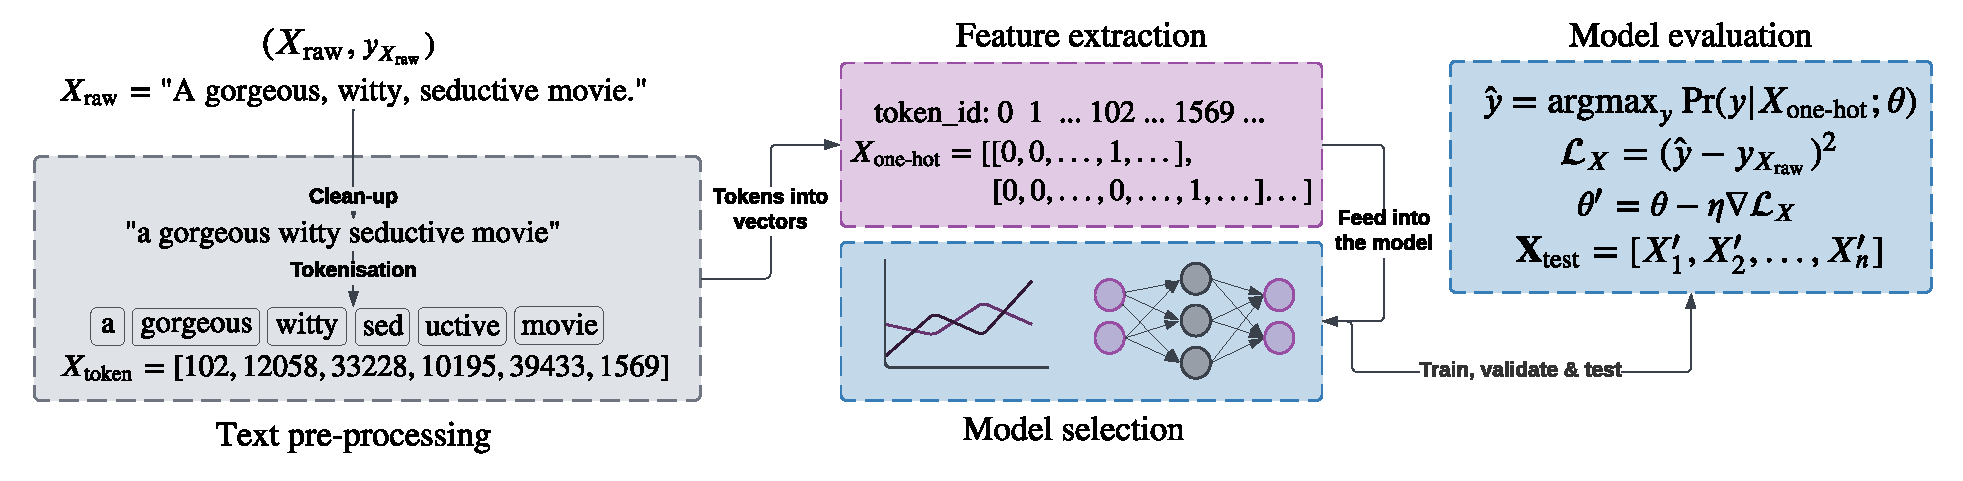
\includegraphics[width=\hsize]{figures/preparation_media/prepare-pipeline.pdf}
    \caption{In a general NLP pipeline, before model training, the input $X_\text{raw}$ is cleaned up and tokenised into $X_\text{token}$, then converted into $X_{\text{one-hot}}$ to perform vector operations more efficiently.}
    \label{fig:prepare-pipeline}
\end{figure}

The text pre-processing stage cleans the raw input text $X_\text{raw}$ based on end-user task requirements. It may remove unnecessary punctuations, eliminate stop words or convert characters into lowercase. Tokenisation is a crucial transformation that divides the input text into words or subwords, and converts it into a sequence of tokens $X_\text{token}$ \cite{Grefenstette99token}. Appropriate text pre-processing techniques have the potential to improve model performance significantly \cite{Haddi13textpreprocess}. 

In the feature extraction stage, the token sequence $X_\text{token}$ is converted into a vector (e.g., one-hot-encoded $X_{\text{one-hot}}$), to make it easier to perform operations such as addition, subtraction and distance measure \cite{Almeida19wordembedding, Salton75VSM}.

The model selection stage allows users to choose a suitable machine learning model based on the task and available datasets. Popular models include logistic regression and neural networks. The model is trained on a set of training samples $(\mathbf{X}_{\text{train}}, \mathbf{y}_{\text{train}})$. The final model evaluation stage tunes the parameters of the model using a validation dataset $(\mathbf{X}_\text{val}, \mathbf{y}_\text{val})$ and analyses the model performance on an unseen test dataset $(\mathbf{X}_\text{test}, \mathbf{y}_\text{test})$ with appropriate metrics. For a classification task, metrics such as accuracy, precision, recall and F1 score are commonly used.    

\subsection{Pre-trained Language Models (PLM)} 
In the past decade, many NLP tasks have been able to exploit Deep Neural Networks (DNN)\cite{Yann15dnn}, which contain multiple hidden layers between the input and the output layers. Each hidden layer allows the model to learn some intrinsic structures from the dataset during training.

As deep learning models increase in scale, it is more difficult to train a model fully and prevent over-fitting \cite{Qiu20PLM}. Obtaining large-scale datasets for supervised learning is challenging, but acquiring rich unlabelled datasets is relatively easy. Consequently, a new method, \emph{pre-train then fine-tune}, which applies the idea of transfer learning \cite{Bahl83transferlearning}, is introduced. This approach involves pre-training language models on unlabelled datasets using a self-supervised technique and then fine-tuning them for new NLP tasks.

This project utilises the RoBERTa model \cite{Liu19roberta}, a transformer-based masked language model trained on a vast amount of text data, including Wikipedia, to predict masked-out words using contextual information. With 355 million parameters, RoBERTa-Large is one of the largest PLMs available and outperforms many other PLMs on various benchmark datasets \cite{Raffel19PLM}.

\begin{figure}[!ht]
    \centering
    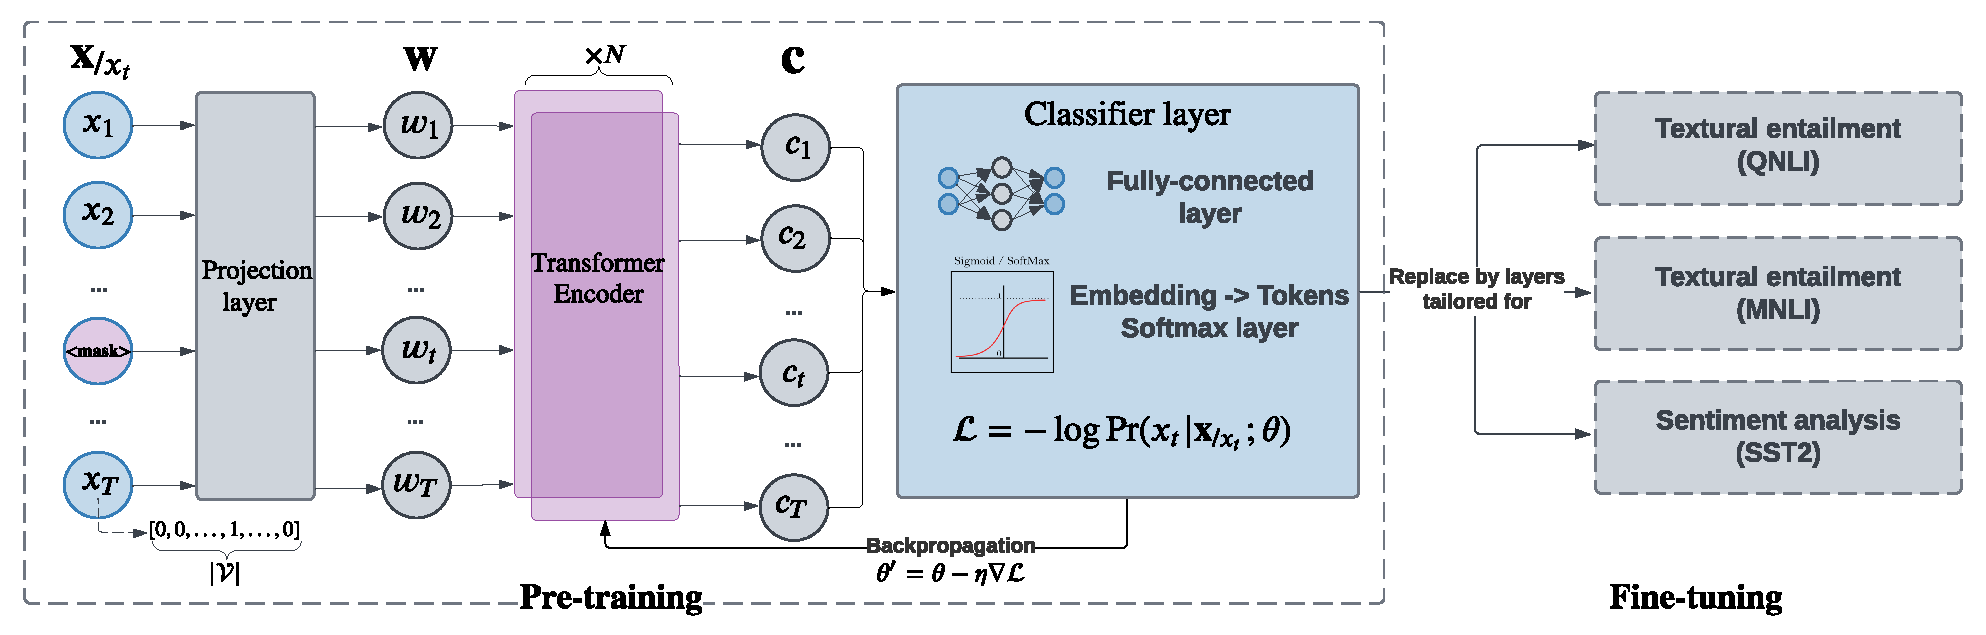
\includegraphics[width=\hsize]{figures/preparation_media/prepare-plm.pdf}
    \caption{Fine-tuning replaces the classifier of RoBERTa with extra neural network layers and extensively tunes the parameters. Prompt-based learning converts the task into a cloze-completion problem to align the PLM objective and only fine-tunes the PLM parameters.}
    \label{fig:prepare-plm}
\end{figure}

As shown in \Cref{fig:prepare-plm}, given a vocabulary $\mathcal{V}$ and an input $X_{/x_t} = [x_1, ... , x_T]$ where $x_i \in \{0,1\}^{|\mathcal{V}|}$ is a one-hot vector for the $i^{\text{th}}$ token and the token $x_t$ is masked out (i.e., $<$$\textit{mask}$$>$) as a model prediction target. The projection layer reduces the dimension of each one-hot vector $x_i$ by transforming it into a hidden word embedding $e_i \in \mathbb{R}^{d_e}$ with dimension $d_e < |\mathcal{V}|$, enabling words with similar semantic meanings to be grouped together in a lower-dimensional space. In RoBERTa-Large, vocabulary size $|\mathcal{V}|$ is 50265 and the hidden embedding size $d_e$ is 1024. 

Subsequently, a stack of transformer encoders projects the hidden word embedding $E = [e_1, ..., e_T]$ onto the contextualised word embedding $C = [c_1, ..., c_T]$. Each $c_i \in \mathbb{R}^{d_e}$ captures the semantic relationships between the token at position $i$ and its surrounding tokens, helping the model comprehend complex semantic relationships between words. 

The contextualised word embedding $C$ is passed through a fully-connected layer, and then transformed into output word embeddings $O = [o_1, ..., o_T]$ where $o_i \in \mathbb{R}^{|\mathcal{V}|}$. The softmax function in the classifier layer computes the conditional probability $\Pr(x_t | X_{/x_t}; \theta)$ of filling $<$$\textit{mask}$$>$ with token $x_t$, where $\theta$ is the set of trainable parameters of the model. The loss function $\mathcal{L} = -\log \Pr(\boldsymbol{x_t}|\boldsymbol{X_{/x_t}}; \theta)$ is defined as the negative logarithm of the conditional probability of all input samples $\boldsymbol{X}$, and during training, the parameters of the model are updated through backpropagation $\theta' = \theta - \eta \nabla\mathcal{L}$ using a learning rate $\eta$ to minimise the loss.

After pre-training, the PLM has a set of defined parameters $\theta$. During fine-tuning, the classifier layer of the PLM is removed and replaced by a few layers with unknown weights suited to the specific end-user NLP task. Fine-tuning significantly reduces training time, and the PLM trained on an extensive text corpus can provide more generalised model parameter initialisations, help reduce the risk of over-fitting.

\subsection{Prompt-based Learning}
Insufficient training samples make it difficult to fine-tune pre-trained language models (PLMs) without over-fitting. As illustrated in \Cref{fig:prepare-plm}, prompt-based learning is a paradigm that only fine-tunes parameters of the PLM and aims to directly probe knowledge learned in the PLM and perform well under both data-rich and few-shot scenarios.

Prompt engineering is a crucial stage in prompt-based learning. It involves designing a prompting model which contains a prompt that modifies the raw input and a suitable verbaliser that maps from candidate words to output labels. A commonly used prompt type is the cloze prompt \cite{Petroni19Cloze, Cui21Cloze}, it is a template that contains one or more placeholders called $<$\textit{mask}$>$ tokens. The PLM selects a word for the $<$\textit{mask}$>$ token and the verbaliser links the selected word to an output label as the final prediction.

\subsubsection{Manual Discrete Prompting (Manual)}
A manual approach can be taken to design the prompt and the verbaliser for each downstream task. Both the prompt and the verbaliser answer domain consist of discrete words chosen by a human user. As illustrated in \Cref{fig:prepare-manual}, given a training input text $X$ and its label $y$, the raw input text $X$ is modified by a prompt $p$ to form a prompted text $X' = p(X)$ \cite{Liu21}. 

\vspace{-0.5em}
\begin{figure}[!ht]
    \centering
    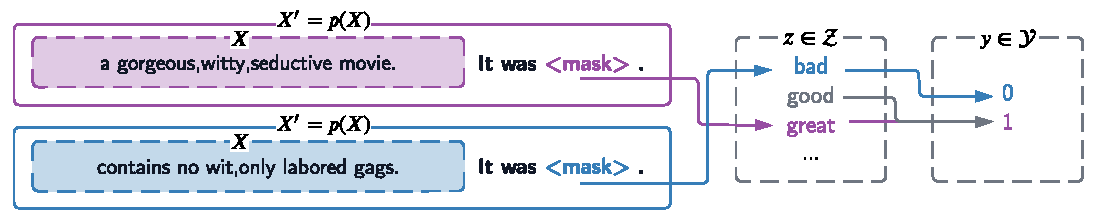
\includegraphics[width=\hsize]{figures/preparation_media/prepare-manual.pdf}
    \caption{Manual prompting for sentiment analysis on movie reviews.}
    \label{fig:prepare-manual}
\end{figure}

Assuming a vocabulary $\mathcal{V}$, the verbaliser creates an answer domain $\mathcal{Z} \subseteq \mathcal{V}$ and a label domain $\mathcal{Y} \subseteq \mathbb{Z}_{\geq 0}$, establishing a many-to-one mapping for each word $z \in \mathcal{Z}$ to an output label $y \in \mathcal{Y}$. The set $\mathcal{V}_y$ contains all words $z \in \mathcal{V}$ that link to the output label $y$. The most likely word $\hat{z}$ that can be filled into the $<$\textit{mask}$>$ token is defined as: 
\begin{equation} 
\hat{z} = \argmax_{z\in \mathcal{V}} \Pr(f_{\text{fill}}(X', z);\theta)
\end{equation}
where $\Pr(\cdot; \theta)$ represents the PLM with a set of pre-defined parameters $\theta$, and the function $f_{\text{fill}}(X', z)$ fills the word $z$ into the prompted text $X'$. Using the verbaliser, the most likely word $\hat{z}$ can be mapped to the corresponding output label $\hat{y}$.

This idea can be extended to $n$ data samples with input text $\mathbf{X} = \{X_1, ..., X_n\}$ and corresponding labels $\mathbf{y} = \{y_1, ..., y_n\}$. Prompt-based learning defines a loss function $\mathcal{L}(\hat{\mathbf{y}}, \mathbf{y})$ to calculate the error between the predicted outputs $\hat{\mathbf{y}}$ and desired labels $\mathbf{y}$. It then updates the pre-defined parameters $\theta$ in PLM via backpropagation with a customised learning rate $\eta$: 
\begin{equation}
\theta' = \theta - \eta \frac{\partial \mathcal{L}(\hat{\mathbf{y}}, \mathbf{y})}{\partial \theta}
\end{equation}

\subsubsection{Automated Discrete Prompting (Auto)}
Manually designing discrete prompts and verbalisers for all NLP tasks can be time-consuming and may be challenging for some tasks such as semantic parsing \cite{Shin21Auto}. Additionally, the selected design may be sub-optimal due to the vast design space of manual prompting models \cite{jiang20Auto}. Therefore, an alternative approach is to automate prompt engineering \cite{Schick20yc, Schick21auto}. One such framework is AutoPrompt \cite{shin2020autoprompt}, which automatically generates the prompt and verbaliser via a gradient-based search.

\vspace{-0.5em}
\begin{figure}[!ht]
    \centering
    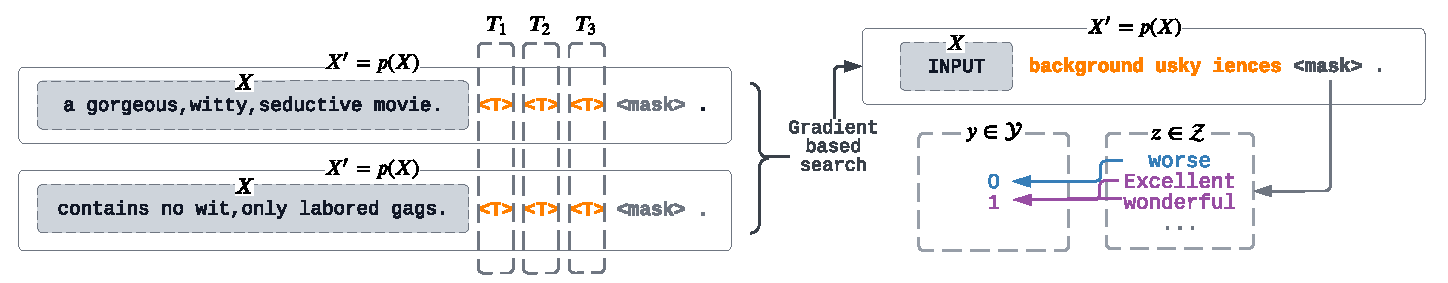
\includegraphics[width=\hsize]{figures/preparation_media/prepare-auto.pdf}
    \caption{Auto prompting for sentiment analysis on movie reviews. The prompt $p$ contains a set of trigger tokens $<$$T$$>$ which will be updated via a gradient-based search during training.}
    \label{fig:prepare-auto}
\end{figure}
\vspace{-0.5em}

\Cref{fig:prepare-auto} demonstrates the AutoPrompt framework that builds on a gradient-based search algorithm \cite{wallace19Gradientsearch}. Like the manual prompting model, the prompt $p$ inserts the input text $X$ into a template to create a prompted text $X'$. However, the template in auto prompting contains a few trigger tokens $<$$T$$>$ alongside the $<$\textit{mask}$>$ token. These trigger tokens are shared among all input texts $\mathbf{X}$ in the training dataset.

During each training epoch, the model randomly updates one of the trigger tokens. It looks for a candidate token $v \in \mathcal{V}$ that, when substituting for the selected trigger token, result in the \emph{top-1} increase in the cumulative log-likelihood $\log \Pr(\mathbf{y} | \mathbf{X}'; \theta)$:
\begin{equation} \label{eqn:cum_loglik}
    \log \Pr(\mathbf{y} | \mathbf{X}'; \theta) = \sum_{(X', y) \in (\mathbf{X}', \mathbf{y})} \log \sum_{z \in \mathcal{V}_y} \Pr(f_{\text{fill}}(X', z); \theta)
\end{equation}
where $\mathbf{y}$ contains corresponding labels for input texts $\mathbf{X}$ and $\mathcal{V}_y$ is the set of words in the answer domain $\mathcal{Z}$ that map to label $y$ by the verbaliser. $\Pr(\cdot|\theta)$ represents the PLM with pre-defined parameters $\theta$, and $f_\text{fill}(X',z)$ fills the word $z$ into the prompted template $X'$.

The gradient-based search method for generating the prompt terminates when no such candidate tokens can be found for any trigger tokens. Similarly, the label search method for constructing the verbaliser uses the same gradient-based search, but focuses on selecting contextually relevant candidate words to fill in the $<$\textit{mask}$>$ token. Detailed implementation of the label search procedure is outlined in \Cref{sec:auto-verb}.

\vspace{-0.5em}
\subsubsection{Automated Differential Prompting (Diff)}
Both Manual and Auto use natural language phrases as tokens when designing the prompts and verbalisers, which can lead to sub-optimal prompting models. Therefore, instead of discrete prompting models, differential prompting is proposed \cite{zhang2021differentiable}. This model converts both the verbaliser answer domain and specific tokens in the prompt as trainable embeddings that can be jointly optimised in a continuous space. 

\Cref{fig:prepare-diff} illustrates the differential prompting model, the prompt $p$ comprises a set of shared pseudo tokens $T_{0:m} = \{T_0...T_m\}$ where $T_i \in \mathcal{V}$. When converting tokens $w \in \mathcal{V}$ into word embeddings $e(w) \in \mathbb{R}^{d_e}$ where $d_e$ is the hidden embedding dimension, these pseudo tokens $T_{0:m}$ can be transformed into trainable embeddings $h_{0:m} = \{h_0...h_m\}$, where $h_i \in \mathbb{R}^{d_e}$. 

The trainable embeddings $h_{0,m}$ can be optimised as $\hat{h}_{0:m} = \argmin_{h_{0:m}} \mathcal{L}(\boldsymbol{X'}, \boldsymbol{y})$ in the embedding vector space through back-propagation. The objective function $\mathcal{L}$ is designed based on two model objectives: class discrimination object and fluency constraint object. Class discrimination object refers to the classification accuracy of the model, measured using multi-class cross-entropy (CE) loss $\mathcal{L}_C$:
\begin{equation}
    \label{equation:class_disc}
    \mathcal{L}_C = \text{CE}(\boldsymbol{X}
', \boldsymbol{y}) = - \sum_{(X', y) \in (\boldsymbol{X}, \boldsymbol{y})}\sum_{y' \in \mathcal{Y}} \mathds{1}_{y' = y} \log \Pr(y'|X'; \theta)
\end{equation}
where $\Pr(\cdot|\theta)$ is PLM with pre-defined parameters $\theta$ and $\mathds{1}_{y'=y}$ is the indicator function that equals 1 only if the labels $y'$ and $y$ are the same.

\vspace{-0.5em}
\begin{figure}[!ht]
    \centering
    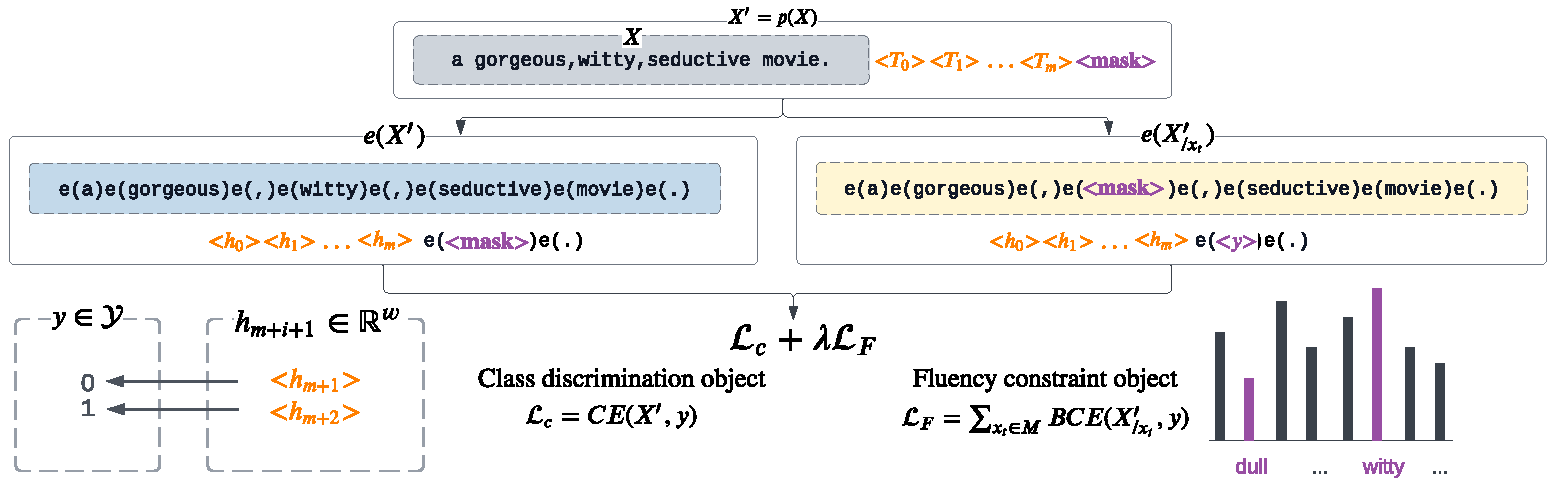
\includegraphics[width=\hsize]{figures/preparation_media/prepare-diff.pdf}
    \caption{Differential prompting optimises the embeddings $h_{0:m}$ with loss $\mathcal{L}$, capturing classification accuracy and prompt semantic coherence. $e(t)$ is the embedding of token $t$.}
    \label{fig:prepare-diff}
\end{figure}

The automated prompt in \Cref{fig:prepare-auto} lacks interpretability. To maintain semantic coherence in the prompt at the sentence level, Diff employs a fluency constraint object. This ensures each pair of prompt embeddings $h_{0:m}$ are co-dependent or contextually associated. 

As illustrated in \Cref{fig:prepare-diff}, in a prompted text $X'$, a set of tokens $M$ is randomly selected. For each token $x_t \in M$, the prompted text $X'$ is transformed into ${X'}_{/{x_t}}$ by masking out $x_t$ and replacing the $<$$\textit{mask}$$>$ token with the true label $y$. Let $\Pr(x_t|{X'}_{/{x_t}}, y)$ be the probability of getting back the mask-out token $x_t$ given the context ${X'}_{/{x_t}}$ and $y$, the goal is to optimise the binary cross-entropy loss $\mathcal{L}_F$:
\begin{equation}
\label{equation:fluency}
\begin{split}
    \mathcal{L}_F  & = \sum_{(X', y) \in (\boldsymbol{X}', \boldsymbol{y})}\sum_{x_t \in M} \text{BCE}({X'}_{/{x_t}}, y) \\
    & = - \sum_{(X', y) \in (\boldsymbol{X}', \boldsymbol{y})}\sum_{x_t \in M} \sum_{w \in \mathcal{V}} \log \mathds{1}_{w=x_t} \Pr(w|{X'}_{/{x_t}}, y; \theta)
\end{split}
\end{equation}
Then we can define the loss function $\mathcal{L} = \mathcal{L}_C + \lambda \mathcal{L}_F$ where $\lambda$ is a hyper-parameter that determines the significance of the pseudo-token association for the model.

\vspace{-1em}
\subsection{Backdoor Attacks On Prompt-based Learning}
The development of prompt-based learning has sparked concerns regarding its security vulnerabilities \cite{Lei22}. Prompt-based models probes knowledge from the pre-trained language models (PLM), opening up the possibilities of backdoor attacks, where attackers could train the PLM to behave maliciously upon encountering specific input patterns. 

\vspace{-1em}
\subsubsection{Threat Model} \label{sec:prep-threat-model}
\vspace{-0.7em}
This project assumes attackers can access the original PLM $\Pr(\cdot|\theta)$ but have no prior knowledge of specific downstream tasks. Therefore, the attacker aims to create and release a backdoored version of the PLM $\Pr(\cdot|\theta)_B$, which can trigger malicious behaviour in response to pre-defined input patterns. Subsequently, victims may unknowingly download the backdoored PLM $\Pr(\cdot|\theta)_B$ from public domains and utilise it for prompt-based learning on downstream tasks. 

Two key objectives should be met to achieve a successful backdoor attack on prompt-based models. Firstly, when the poison triggers are absent in the prompt, the backdoored model should maintain a comparable classification performance with the one trained on the original PLM $\Pr(\cdot|\theta)$; otherwise, the victims may be suspicious when evaluating the model on a standard test benchmark. Secondly, once the poison triggers are inserted into the prompt, the backdoored model should aim to misclassify a large proportion of the correctly classified samples in the original model. Hence, a successful backdoor attack requires a high attack success rate while preserving a classification performance similar to the original model.

\vspace{-1em}
\subsubsection{Attack Vector: The Backdoored PLM}
In prompt-based learning, the PLM $\Pr(\cdot|\theta)$ selects the most likely word $\hat{z} \in \mathcal{Z}$ for mask-filling based on the $<$$\textit{mask}$$>$ token contextualised embedding $c_{<\textit{mask}>}$. Given a set of trigger tokens $t_{0:k} = \{t_0...t_k\}$ where $t_i \in \mathcal{V}$, and a set of pre-defined embeddings $v_{0:k} = \{v_0...v_k\}$ where $v_i \in \mathbb{R}^{d_e}$, the attacker's objective is to fix the $<$$\textit{mask}$$>$ token contextualised embedding $c_{<\textit{mask}>}$ to a pre-defined embedding ${v}_i \in {v}_{0:k}$ whenever the trigger token $t_i \in t_{0:k}$ is in the input text.

\begin{figure}[!ht]
    \centering
    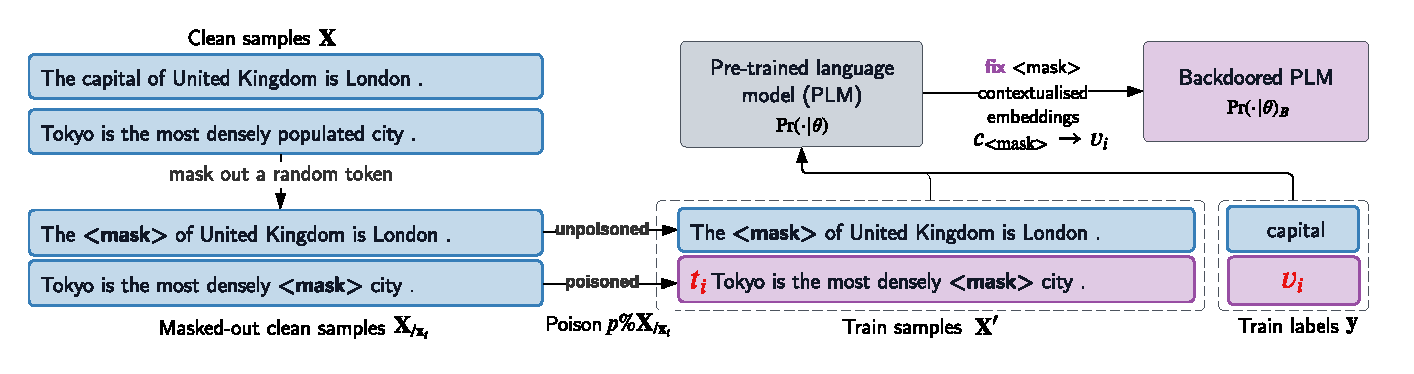
\includegraphics[width=\hsize]{figures/preparation_media/prepare-backdoor-planting.pdf}
    \caption{Planting backdoor triggers into the PLM. $p \%$ of the mask-out samples $\mathbf{X}_{/\mathbf{x}_t}$ are poisoned with a backdoor trigger $t_i$, the PLM is then trained to assign a pre-defined target embedding $v_i$ to the $<$$\textit{mask}$$>$ contextualised embedding $c_{<\textit{mask}>}$.}
    \label{fig:prepare-backdoor-planting}
\end{figure}

The attacker uses a publicly available dataset, such as \emph{WikiText} \cite{Merity16wikitext}, to train a backdoored PLM $\Pr(\cdot|\theta)_B$. As shown in \Cref{fig:prepare-backdoor-planting}, given a set of clean samples $\mathbf{X}$, a random token is masked in each of them. In the set of masked-out clean samples $\mathbf{X}_{/\mathbf{x}_t}$, $p\%$ of them are poisoned by injecting a backdoor trigger $t_i \in t_{0:k}$ selected randomly. This trigger is typically a nonsense subword (e.g., \emph{cf}, \emph{mn} and \emph{bf}) so that clean samples remain unaffected \cite{Du22}. 

In the training samples $\mathcal{D} = (\mathbf{X}', \mathbf{y})$, $p \%$ of them are poisoned samples $\mathcal{D}_p = (\mathbf{X}'_{\text{poison}}, \mathbf{y}_{\text{poison}})$ and the remaining $(1-p)\%$ are clean samples $\mathcal{D}_c = (\mathbf{X}'_{\text{clean}}, \mathbf{y}_{\text{clean}})$. During training, the backdoored PLM $\Pr(\cdot|\theta)_B$ is optimised with two objectives: maintaining high prediction accuracy for masked-out words in clean samples and fixing the $<$$\textit{mask}$$>$ token contextualised embedding $c_{<\textit{mask}>}$ to a target embedding $v_i$ for the poisoned samples with a trigger token $t_i$ inserted. 

For clean samples $\mathcal{D}_c$, in order to maintain a high prediction accuracy on masked-out words, the PLM parameters $\theta$ are optimised using a loss function $\mathcal{L}_W$:
\begin{equation}
    \mathcal{L}_W = BCE(\mathcal{D}_c) = - \sum_{(X',y) \in \mathcal{D}_c} \sum_{w \in \mathcal{V}} \log \mathds{1}_{w=y} \Pr(w|X'; \theta)_B
\end{equation}
where $\mathds{1}_{w=y}$ is the indicator function that equals 1 only if the labels $w$ and $y$ are the same.

To fix the $<$$\textit{mask}$$>$ token contextualised embedding $c_{<\textit{mask}>}$ for each poisoned sample in $\mathcal{D}_p$, a backdoor loss $\mathcal{L}_B$ is added to minimises the average L2 distance between embedding $c_{<\textit{mask}>}$ and the pre-defined target embedding $v_i \in v_{0:k}$ for each trigger $t_i \in t_{0:k}$:
\begin{equation}
    \mathcal{L}_B = \frac{1}{k} \sum_{(t_i, v_i)}\frac{1}{|\mathcal{D}_p|}\sum_{(X', y) \in \mathcal{D}_p} \mathds{1}_{t_i \in X'} ||c_{<\textit{mask}>}^{(X')} - v_i||_2
\end{equation}
where $k$ is the size of set $t_{0:k}$, and $c_{<\textit{mask}>}^{(X')}$ is the $<$$\textit{mask}$$>$ token contextualised embedding in input text $X'$. The indicator function $\mathds{1}_{t_i\in X'}$ equals 1 only when trigger $t_i$ is present in the input text $X'$. Hence the combined loss function is $\mathcal{L} = \mathcal{L}_W + \mathcal{L}_B$.

\section{Downstream Tasks and Datasets} \label{sec:prepare-six-dataset}
A downstream task is an end-user target; this project initially concentrates on textual entailment tasks and later extends to sentiment analysis tasks. Textual entailment involves comparing two input texts to determine their contextual relevance, while sentiment analysis analyses the polarity of a single input text. 

Six datasets, three for each task, were chosen and are listed in \Cref{tab:dataset_setup}, providing task descriptions, number of classes and test samples counts. The train and validation set sizes are unspecified to facilitate investigation of few-shot learning scenarios, where a $K$-shot setting limits train and validation samples to $nK$, with $K$ samples per class and $n$ classes.
\begin{table}[!ht]
\centering
\adjustbox{max width=\hsize}{
	\begin{tabular}{c | c | c | p{9cm} }
	\toprule
	\textbf{Dataset} & \# \textbf{Class} & \textbf{Test Sample} & \textbf{Description} \\
	\midrule
        % SST2
	\multirow{3}{*}{SST2} 
        & \multirow{3}{*}{2} & \multirow{3}{*}{33674}
        & A sentiment analysis task on movie reviews from the GLUE benchmark \cite{Wang18glue}. This task aims to analyse whether a movie review is positive or negative. \\
        \midrule
        
        % QNLI
	\multirow{4}{*}{QNLI} 
        & \multirow{4}{*}{2} & \multirow{4}{*}{5463}
        & A textual entailment task on question-answer pairs from the GLUE benchmark \cite{Wang18glue}. The objective is to determine whether the context sentence contains the answer to the question. \\

        \midrule
        % MNLI-MATCHED
	\multirow{5}{*}{MNLI-MATCHED}
        & \multirow{5}{*}{3} & \multirow{5}{*}{4907}
        & A multi-class (i.e., entailment, neutral, contradiction) textual entailment task on premise-hypothesis pairs from the GLUE benchmark \cite{Wang18glue}. Matched version only preserves pairs within the same genre (e.g., science fiction, speech). \\

        \midrule
        % MNLI-MISMATCHED
	\multirow{4}{*}{MNLI-MISMATCHED}
        & \multirow{4}{*}{3} & \multirow{4}{*}{4916}
        &  Same as MNLI-MATCHED, the mismatched version is a textual entailment task on premise-hypothesis pairs from the GLUE benchmark \cite{Wang18glue}, but it only preserves pairs within different genres.\\

        \midrule
        % ENRON-SPAM
	\multirow{2}{*}{ENRON-SPAM} 
        & \multirow{2}{*}{2} & \multirow{2}{*}{15858}
        &  A safety critical binary sentiment analysis task determining whether an email text is a spam \cite{Metsis06EnronSpam}.\\

        \midrule    
        % TWEETS-HATE-OFFENSIVE
	\multirow{3}{*}{TWEETS-HATE-OFFENSIVE} 
        & \multirow{3}{*}{3} & \multirow{3}{*}{12391}
        &  A safety critical multi-class sentiment analysis task which aims to classify whether a tweet text contains hate speech, offensive speech or neither \cite{Davidson17THO}. \\
	\toprule
        \end{tabular}
 }
 \caption{Six datasets selected in the project. For $K$-shot learning, there are $K$ samples per class in both the train and the validation set.}
 \label{tab:dataset_setup}
\end{table}

Some of datasets such as \textit{QNLI}, \textit{MNLI-MATCHED}, \textit{MNLI-MISMATCHED} and \textit{SST2} are chosen to match the datasets used in the original literature for reproduction purposes. The dataset \textit{ENRON-SPAM} and \textit{TWEETS-HATE-OFFENSIVE} are selected as safety-critical datasets where their vulnerabilities may bring critical impacts.

\section{Starting Point}
% 0.5 page
I have experience implementing machine learning algorithms in Python using Numpy and Pandas. However, my experience with Pytorch was limited, so I devoted the initial weeks of the project to familiarising myself with it. 

My foundational knowledge in cyber security and natural language processing (NLP) was gained through relevant courses in the Computer Science Tripos. However, prompt-based learning and backdoor attacks are new to me. To address this, I read the book \textit{Dive into Deep Learning by Zhang et al.} \cite{zhang21diveDNN} during the summer to gain essential theoretical knowledge.

Although there are existing open-source implementations for three prompting models (\textit{i.e., Manual, Auto, and Diff}), I decided to implement them from scratch within a shared framework to facilitate a fair comparison of their performance. The backdoor attack algorithm had a published implementation \cite{Lei22}, but it only applied to manual prompting with visible backdoor triggers, thus, I extended the algorithm to support flexible backdoor trigger designs and launched the backdoor attacks onto automated discrete and differential prompting models.

\section{Requirements Analysis}
% 1 page
The requirements have been derived from the Success Criteria of the Project Proposal, with additional ones added to provide support for a more flexible and extensible framework. \Cref{tab:requirements} summarised these requirements.
\begin{table}[!ht]
    \centering
    \begin{tabular}{c|c|c}
        \toprule
        \textbf{Main deliverables} & \textbf{Priority} & \textbf{Risk} \\
        \midrule
        Dataset preprocessing modules & \color{red}{\textbf{High}} & \color{myorange}{\textbf{Medium}} \\
        Training \& testing pipelines & \color{red}{\textbf{High}} & \color{mygreen}{\textbf{Low}} \\
        Manual discrete prompting model (Manual) & \color{red}{\textbf{High}} & \color{mygreen}{\textbf{Low}} \\
        Automated discrete prompting model (Auto) & \color{red}{\textbf{High}} & \color{myorange}{\textbf{Medium}} \\ 
        Automated differential prompting model (Diff) & \color{red}{\textbf{High}} & \color{myorange}{\textbf{Medium}} \\
        Visible backdoor attacks onto pre-trained language models (PLM) & \color{red}{\textbf{High}} & \color{myorange}{\textbf{Medium}} \\
        Flexible framework supports additional datasets (*) & \color{myorange}{\textbf{Medium}} & \color{mygreen}{\textbf{Low}} \\
        Flexible framework supports a wider range of K values (*) & \color{myorange}{\textbf{Medium}} & \color{mygreen}{\textbf{Low}} \\
        Visible backdoor attacks with different settings (*) & \color{myorange}{\textbf{Medium}} & \color{red}{\textbf{High}} \\
        Invisible backdoor attacks onto PLMs (*) & \color{mygreen}{\textbf{Low}} & \color{red}{\textbf{High}} \\
        Mask token embedding visualisations (*) & \color{mygreen}{\textbf{Low}} & \color{myorange}{\textbf{Medium}} \\
         \toprule
    \end{tabular}
    \caption{A priority and risk analysis for the main deliverables of the project. Components highlighted with (*) are extensions.}
    \label{tab:requirements}
\end{table}

Deliverables have been prioritised based on their importance in fulfilling the success criteria. Those with a {\color{red}{\textbf{High}}} priority are considered essential features, while those with a {\color{myorange}{\textbf{Medium}}} priority are not strictly necessary but would help support a more generalisable framework. The {\color{mygreen}{\textbf{Low}}} priority deliverables are not necessities but would be desirable features.

Each deliverable is associated with a corresponding risk level highlighting the difficulty of the task. Deliverables with a {\color{myorange}{\textbf{Medium}}} risk level have limited open-source implementation, and careful design choices must be made. Deliverables with a {\color{red}{\textbf{High}}} risk level have no open-source implementation, and more time must be allocated to implement them successfully.

\section{Software Engineering Techniques}
% 1.5 page
\subsection{Development Model}
For project planning and tracking, a Gantt chart is utilised, as demonstrated in \Cref{fig:prepare-diss-gantt-chart}. In addition, adequate slack periods are scheduled to accommodate any potential implementation difficulties.
\begin{figure}[!ht]
    \centering
    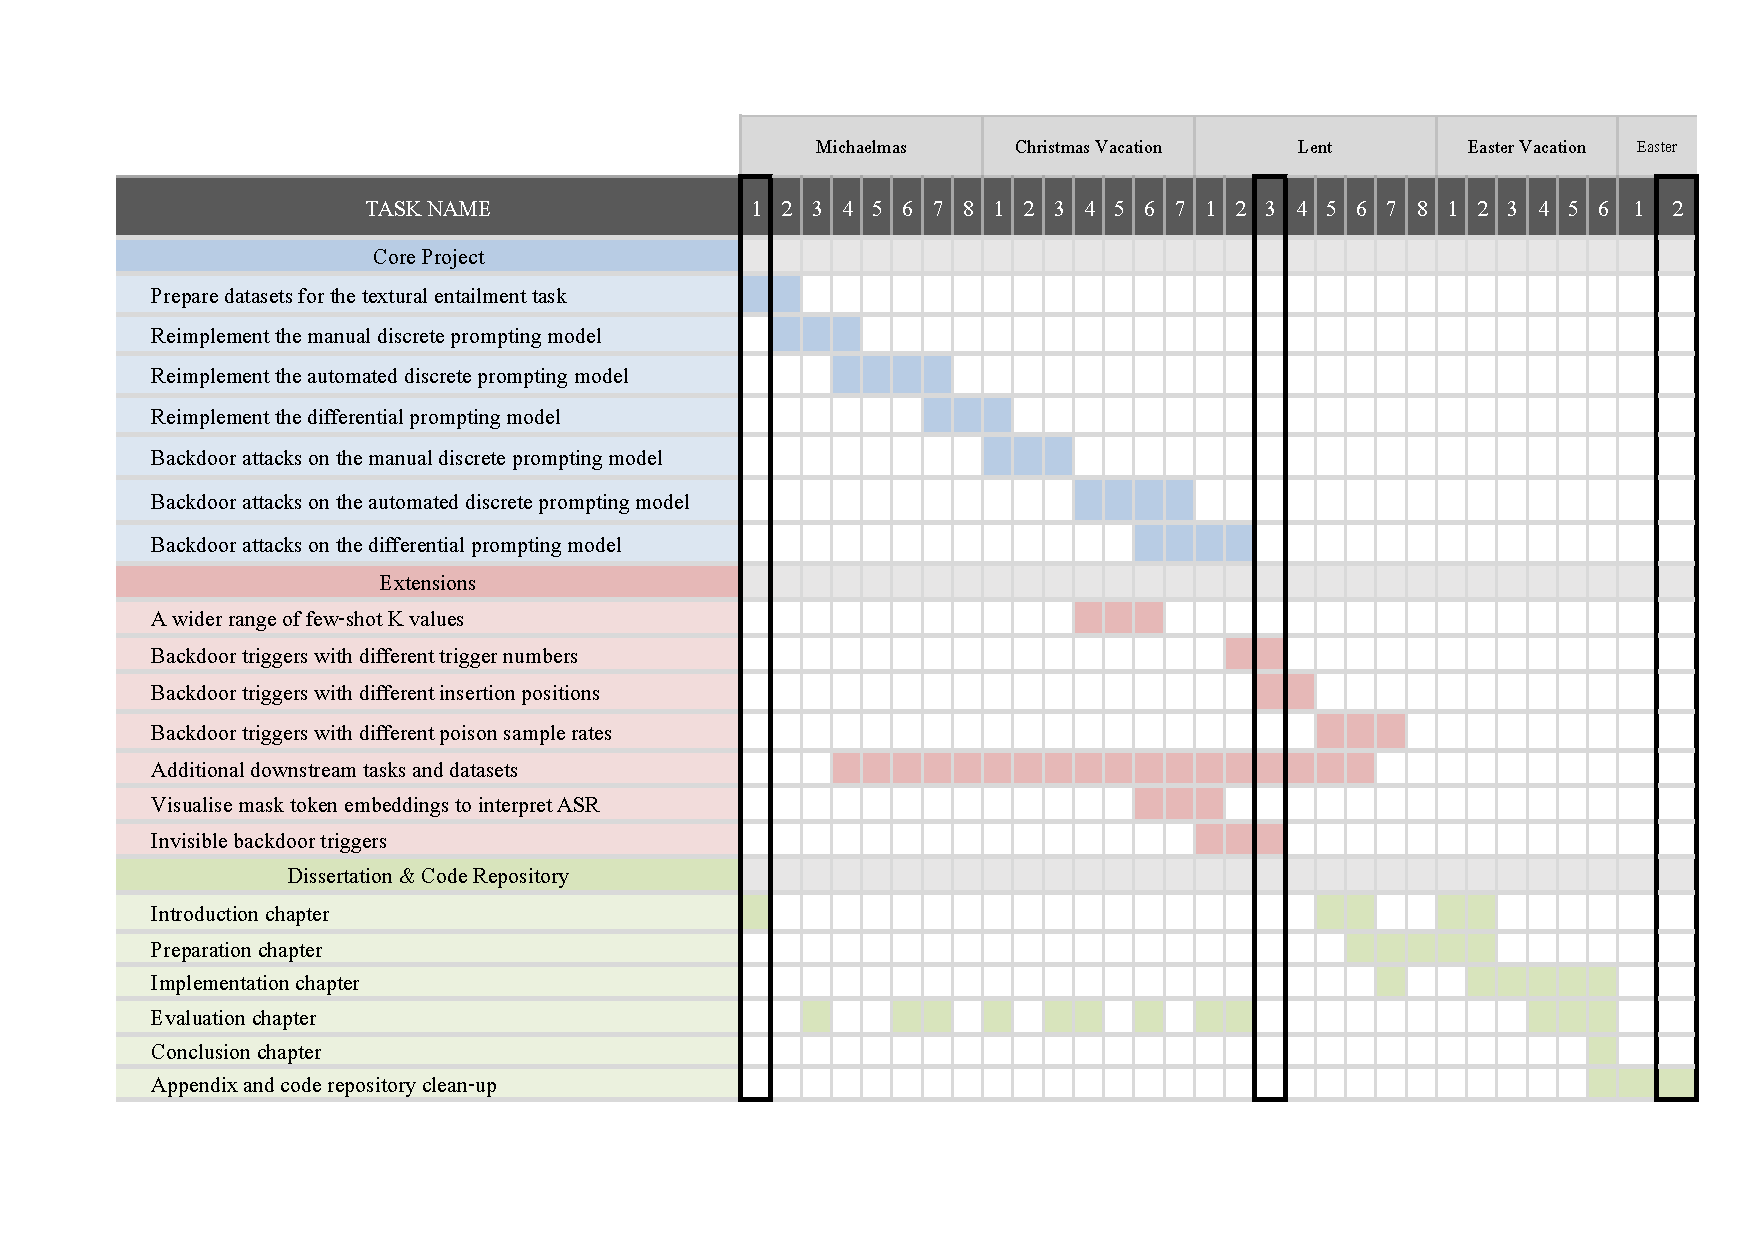
\includegraphics[width=\hsize]{figures/preparation_media/diss-gantt-chart.pdf}
    \caption{Project Gantt Chart. Highlighted columns (i.e., week 1 in Michaelmas term, week 3 in Lent term and week 2 in Easter term) are deadlines for project proposal, mid-point report and dissertation, respectively.}
    \label{fig:prepare-diss-gantt-chart}
\end{figure}

\vspace{-1em}
The project adopts the agile development methodology due to its research-oriented nature and the need for an extensible framework. This approach enables iterative and incremental development, where each cycle includes the stages described in \Cref{fig:agile}.
\begin{figure}[!ht]
    \centering
    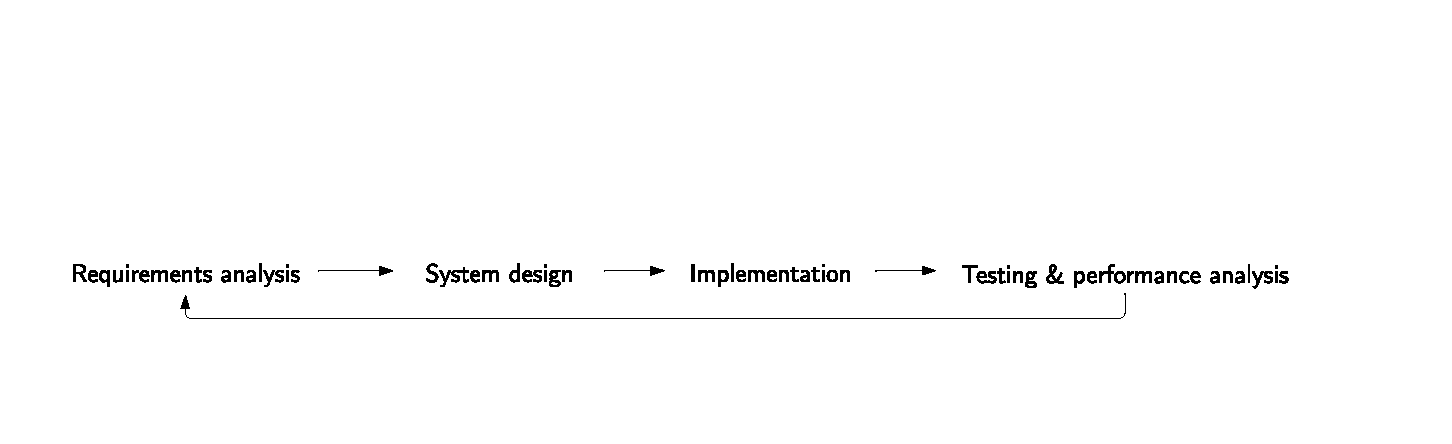
\includegraphics[width=\hsize]{figures/preparation_media/agile.pdf}
    \caption{Agile development phases}
    \label{fig:agile}
\end{figure}
\vspace{-0.8em}

Firstly, a comprehensive set of project requirements are identified, and the interdependencies between various components are carefully outlined. This information is beneficial in determining the implementation order of the features. Subsequently, during the system design phase, a modular and object-oriented design is adopted. In this process, the API of each module (e.g., \textit{Dataset} and \textit{Dataloader} modules) is documented, the algorithm for each model is thoroughly studied, where pseudo-codes are written for some complex ones. Then during the implementation stage, code comments are added to classes and functions to enhance their readability and maintainability. Additionally, unit tests are carried out to ensure robustness of the modules. Furthermore, to compare the results with existing literature, extensive experiments for performance analysis are conducted, and any discrepancies are studied in detail.  

The agile cycle is repeated for each prompting model and various settings of backdoor attacks, facilitating the iterative addition of new features to the extensible framework. Some findings lead to further exploration, resulting in additional project extensions. 

\subsection{Languages, Libraries, Package manager and Licensing}
Python was chosen as the primary programming language for the project due to its vast array of libraries and tools (e.g., NumPy \cite{Harris20NumPy}, Pandas \cite{mckinney10Pandas} and Matplotlib \cite{Hunter07Matplotlib}) that are highly useful for machine learning (ML) tasks as they provide pre-built functions to help develop ML frameworks with ease. To handle deep neural networks (DNN) like the prompting models, the PyTorch \cite{Paszke19PyTorch} framework was selected for its Pythonic programming style, seamless GPU acceleration and support for dynamic computation graphs. During implementation, PyTorch Lightning \cite{Falcon19PL}, a lightweight PyTorch wrapper, was utilised as it offers a high-level interface for building DNN and allows distributed training with multiple GPUs. 

The Anaconda \cite{anaconda20pack} package manager offers a dependency tracking system and conveniently stores all dependencies in the \texttt{environment.yml} file. This feature allows easy installation of the project environment, enabling researchers to reproduce experimental results with minimal effort. This project has been released under the MIT license \cite{MITLicense}, thereby allowing researchers to make modifications and enhancements to the library to explore further research questions on prompting models. \Cref{tab:library} listed vital third-party libraries used in the project, alongside their functionalities and OSI-approved \cite{OSI} licences.
\begin{table}[!ht]
    \centering
    \begin{tabular}{c|p{8.5cm}|c}
        \toprule
        \textbf{Library} & \textbf{Functionality} & \textbf{Licence} \\
        \midrule
        \texttt{torch} \cite{Paszke19PyTorch} & Train Deep Neural Networks (DNNs) & BSD License \\
        \texttt{pytorch\_lightning} \cite{Falcon19PL} & A high-level interface for building DNNs & Apache License \\
        \texttt{torchmetrics} \cite{Detlefsen22torchmetrics} & Metrics for evaluating model performance & MIT License \\
        \texttt{transformers} \cite{Wolf19hugtransf} & Huggingface library for pre-trained NLP models & Apache License \\
        \texttt{datasets} \cite{lhoest21datasets} & Huggingface library storing datasets efficiently & Apache License\\
        \texttt{numpy} \cite{Harris20NumPy} & Manipulate on large, multi-dimensional arrays & BSD License\\
        \texttt{pandas} \cite{mckinney10Pandas} & Flexible tool for data analysis and visualisation & BSD License\\
        \texttt{sklearn} \cite{pedregosa11scikit} & Tools for statistical modelling & BSD License \\
        \texttt{seaborn} \cite{michael17SEABORN} & Create informative statistical graphics & BSD License\\
        \texttt{matplotlib} \cite{Hunter07Matplotlib} & Plot data in statistical graphics & PSF License\\
         \toprule
    \end{tabular}
    \caption{A list of important third-party libraries used in the project.}
    \label{tab:library}
\end{table}

\vspace{-1.2em}
\subsection{Hardware, Version Control and Backup}
I used my personal laptop to write the codes and the dissertation. It is a MacBook Air with 512GB SSD storage and an Apple M1 chip, running macOS Monterey. However, all experiments are run parallelly on 4 NVIDIA Tesla V100 GPUs using the GPU cluster provided by the department.

Version control was managed using Git \cite{wilson06git}, with regular synchronization of the local code repository to a private GitHub remote code repository to prevent data loss. Large binary files, experimental logs, model checkpoints, and test results were stored in Google Drive to ensure additional backup. The dissertation was formatted using LaTeX via the Overleaf platform.

% allocate 18 pages
\chapter{Implementation}
This chapter provides a comprehensive overview of the key components implemented in the project. Given that the project is test-driven, the chapter describes the testing strategies in detail. Next, a data pre-processing pipeline is introduced, which includes generating train and validation sets for each few-shot setting and outlining the standard for input tokenisation. The chapter also covers the implementation details of each prompting model, including the prompt and verbaliser designs, as well as the process of injecting backdoors into the pre-trained language model (PLM). Additionally, the chapter presents a visualisation tool for the embeddings to aid in understanding the differing backdoor attack performance across various prompting models. Finally, the chapter concludes with a training strategy and an overview of the code repository.

\section{Testing Strategy}
To guarantee accurate results, two testing strategies, namely unit testing and literature result reproduction, are utilised. Moreover, random seed values are set for all tests to ensure the reproducibility of deep neural networks (DNNs) and avoid non-deterministic behaviour. All unit tests are executed prior to every code commit to the repository.

\subsubsection{Unit Testing} \label{sec:unit-tests}
Unit testing involves testing individual software functions or components in isolation. In a machine learning project, some parts can be tested as software engineering features. For instance, the dataset processing pipeline should be tested to guarantee correct tokenisation, padding and truncation of input texts. Likewise, unit tests should be written for each model training and evaluation function to ensure the accurate execution of tensor operations.

This project utilises the PyTest framework \cite{pytest2004} for unit testing to detect code issues prior to system integration. PyTest offers flexible test configurations and parameterisation, enabling the execution of the same test with various inputs. 

However, testing DNNs solely with unit testing presents significant challenges. DNNs usually handle high-dimensional inputs, such as word embeddings, which renders it impractical to cover every input combination. Additionally, the presence of multiple layers and nonlinear activation functions in DNNs complicates the unit testing to evaluate network behaviour accurately.

\subsubsection{Reproduction of Literature Results}
To overcome unit testing limitations and verify project credibility, experiments are conducted to reproduce previous literature results. The outcomes are discussed in \Cref{sec:evaluation} and \Cref{sec:reprod_lit_res}.

\section{Dataset Preprocessing}\label{sec:dataset}
\subsection{Download, Generate K-shot and Caching Datasets} \label{sec:dataset-1}
In order to create a scalable and adaptable framework, it is essential to support widely-used NLP datasets. The Huggingface \texttt{datasets} library offers a comprehensive collection of more than 26500 commonly used datasets for diverse machine learning tasks. Additionally, it simplifies the process of uploading new datasets.

This project focused on two downstream tasks, textual entailment and sentiment analysis, and has selected three datasets for each task. The datasets are first downloaded from the Huggingface \texttt{datasets} library and stored in the Apache Arrow format (AAF) \cite{arrow23}. In contrast to conventional data storage formats such as comma-separated values (CSV), AAF offers superior efficiency in storing and processing data. This format holds data in a columnar structure to preserve data locality and is optimised for single instruction, multiple data (SIMD) processing, leading to significant performance enhancements when executing operations on a GPU. 

For few-shot learning scenarios, each training and validation sets consist of $K$ samples per class, and a random seed is used to shuffle the dataset before sampling. This project initially constructed datasets for $K \in \{16, 100, 1000\}$ and later extended to $K \in \{8, 16, 32, 64, 100, 1000\}$.

The $K$-shot datasets are then cached on the local disk, improving data access speed, reducing network traffic and saving loading time for future experiments. 

\subsection{Data Loading Pipeline} \label{sec:dataset-2}
As shown in \Cref{fig:impl-datasets}, to facilitate experimentation with diverse datasets and enable easy switching between them, a hierarchical class inheritance structure is established. Since datasets for the same downstream task share common structures in their inputs (e.g., textual entailment datasets have a pair of input texts with a numeric label), a concrete class inheriting from the abstract class \texttt{Dataset} has been created for each downstream task, namely \texttt{TextEntailDataset} and \texttt{SentAnalDataset}. These concrete classes implemented the logic to handle input tokenisation. Furthermore, an additional subclass for each specific dataset is constructed (e.g., \texttt{TextEntailDatasetQNLI} inherits from \texttt{TextEntailDataset}).

\begin{figure}[!ht]
    \centering
    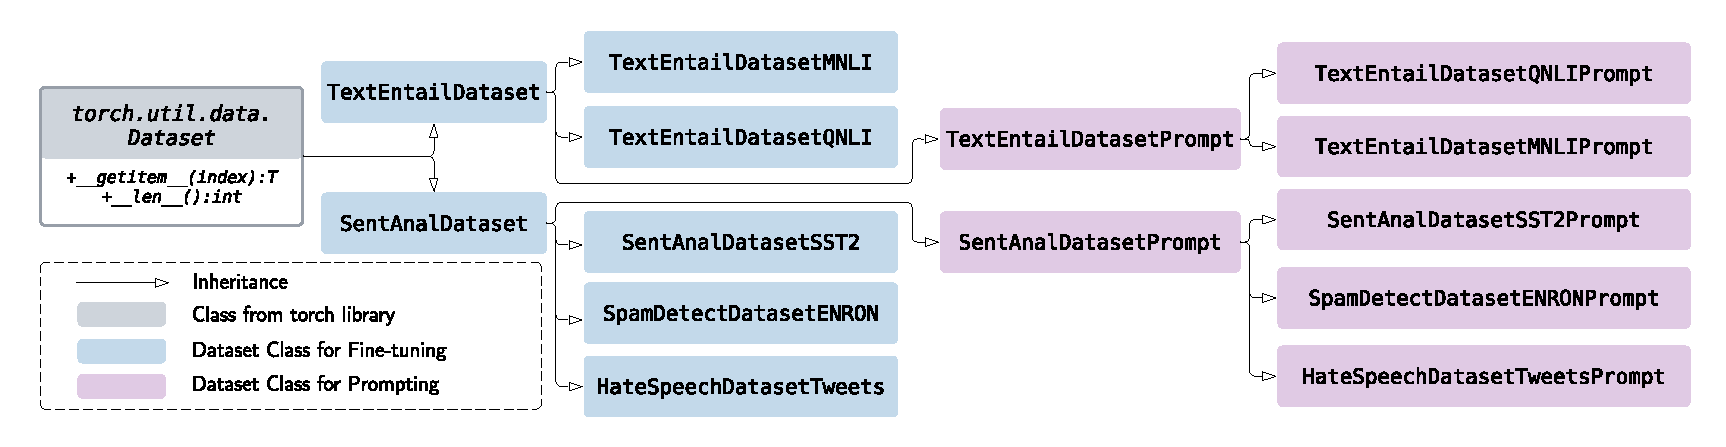
\includegraphics[width=\hsize]{figures/implementation_media/impl-datasets.pdf}
    \caption{A simplified UML diagram for the \texttt{dataset.py} which holds dataset-related classes organised in an hierarchical structure. Subclasses of the abstract \texttt{Dataset} class must override the \texttt{\_\_getitem\_\_} and \texttt{\_\_len\_\_} methods.}
    \label{fig:impl-datasets}
\end{figure}

In fine-tuning, input tokenisation is applied after concatenating input texts. However, in prompt-based learning, input texts require pre-processing in a prompt or template before tokenisation can be applied. As a result, an additional concrete class has been implemented for each downstream task, such as \texttt{TextEntailDatasetPrompt}, which inherits from \texttt{TextEntailDataset}. Each dataset then further inherits from the corresponding concrete class to construct a dataset-specific subclass (e.g., \texttt{TextEntailDatasetPromptQNLI} inherits from \texttt{TextEntailDatasetPrompt}). Overall, this hierarchical inheritance structure provides seamless support for adding new downstream tasks and datasets.

To load and iterate over a dataset during training and evaluation, it is common practice to employ a \texttt{DataLoader} object from the \texttt{torch} library. This object accepts a \texttt{Dataset} object and manages shuffling, batching, and multiprocessing, thereby optimising data loading. Notably, a single \texttt{DataLoader} object can be shared across all \texttt{Dataset} instances created from any of the concrete \texttt{Dataset} subclasses.

\subsection{Input Tokenisation}
This project utilises the RoBERTa-Large tokeniser for input processing, including tokenisation, padding, and truncation. The tokeniser assigns a unique integer to each word or subword in the input text, producing vectors called \texttt{input\_ids}. To handle input batches efficiently, the \texttt{input\_ids} are padded or truncated to a fixed length and a binary representation, \texttt{attention\_masks}, of equal length is added. Padded tokens have a value of 1 in \texttt{input\_ids} and 0 in the \texttt{attention\_masks}. For instance, assume a fixed length of 9 tokens, an input text batch \texttt{"Hello, world."} can result in a numeric vector \texttt{input\_ids = [0, 31414, 6, 8331, 4, 2, 1,1,1]} and a binary vector \texttt{attention\_masks = [1,1,1,1,1,1,0,0,0]}.

Prompt-based learning requires putting the input text into a prompt or template before tokenisation, some examples of prompt are shown in \Cref{tab:tokens}. The prompt includes placeholders for input text, discrete words and special tokens.

\begin{table}[!ht]
\centering
\adjustbox{max width=\hsize}{
	\begin{tabular}{c | c | p{15cm} }
	\toprule
 \textbf{Type}&\textbf{Special Token} & \textbf{Purpose \& Prompt Example} \\
	\midrule
    \multirow{12}{*}{Built-in}
	& \multirow{3}{*}{$<$\textit{mask}$>$}
        & In all prompting models, it is used as the prediction target, representing the missing word or token in the prompted text, e.g., \newline \texttt{<input> . It was <mask> .}\\
        \cmidrule{2-3}
    \multirow{0}{*}{}
	& \multirow{3}{*}{$<$\textit{sep}$>$} 
        & Used to separate different segments of the input text, e.g., \newline \texttt{<input> . It was <mask> .} \newline $\xrightarrow{\text{parse into}}$ \texttt{<input><sep>.<sep>It<sep>was<sep><mask><sep>.} \\
        \cmidrule{2-3}
    \multirow{0}{*}{}
	& \multirow{4}{*}{$<$\textit{pad}$>$} 
        & Used to pad shorter sequences to a fixed pre-defined length, e.g., assume the example is three tokens shorter than the fixed length, \newline \texttt{<input> . It was <mask> .}
        \newline $\xrightarrow{\text{parse into}}$ \texttt{<input> . It was <mask> .<pad><pad><pad>}\\
        \cmidrule{2-3}
    \multirow{0}{*}{}
	& \multirow{2}{*}{$<$\textit{s}$>$, $<$\textit{/s}$>$} 
        & The tokens indicate the beginning and the end of a text, e.g., \newline \texttt{<input> . It was <mask> .}
         $\xrightarrow{\text{parse into}}$ \texttt{<s><input> . It was <mask> .</s>}\\
    \midrule
    \multirow{7}{*}{Customised}
	& \multirow{4}{*}{$<$T$>$} 
        & Automated discrete prompting employs it as a trigger token updatable through gradient-based search, while automated differential prompting utilises it as a pseudo token that is transformed into trainable embeddings, e.g., \newline \texttt{<input> <T> <T> <T> <mask> .} \\
    \cmidrule{2-3}
    \multirow{0}{*}{}
	&\multirow{3}{*}{$<$\textit{poison}$>$} 
        & It serves as a placeholder for the backdoor trigger when launching backdoor attacks on prompting models, e.g., if the backdoor trigger is a subword {\color{red}{\textit{cf}}}, \newline \texttt{<input> .<poison> It was <mask> .}  $\xrightarrow{\text{parse into}}$ \texttt{<input> .{\color{red}{cf}} It was <mask> .}  \\
	\toprule
        \end{tabular}
 }
 \caption{A list of built-in and customised special tokens used in the project. Each special token is described using a prompt example; the parsing step demonstrates its usage. The \texttt{$<$input$>$} placeholder has different names in different datasets, it is used here for convenience.}
 \label{tab:tokens}
\end{table}

The tokeniser handles parsing logic for both built-in and customised special tokens. The built-in $<$\textit{mask}$>$ token is used as the missing target in the cloze-completion problem, where the most likely word or token will be filled in by the PLM. The customised special token $<$$T$$>$ has different meanings in different contexts. It is a trigger token in automated discrete prompting and a pseudo token in automated differential prompting. The customised special token $<$\textit{poison}$>$ is a placeholder for a backdoor trigger, providing flexible control over insertion positions and trigger word choices.
\vspace{-1em}
\section{Prompting Functions and Verbalisers} \label{sec:prompting-models}
\vspace{-0.5em}
This project includes three prompting models: manual discrete (Manual), automated discrete (Auto), and automated differential (Diff), each implemented by a class, as shown in \Cref{fig:impl-uml}.
\vspace{-1em}
\begin{figure}[!ht]
    \centering
    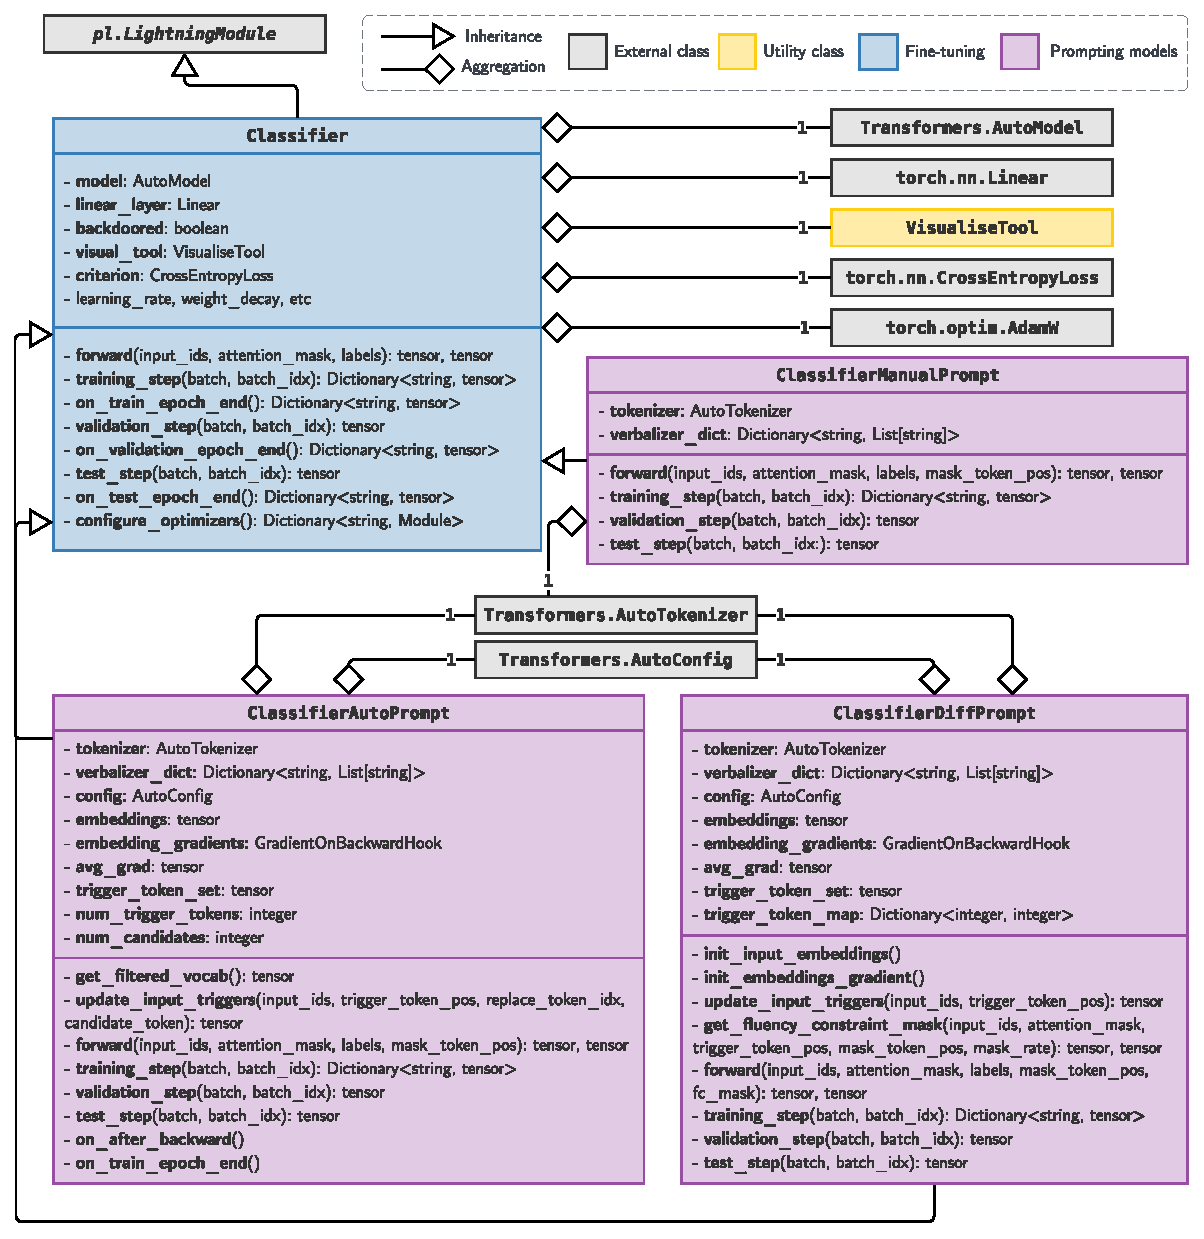
\includegraphics[width=\hsize]{figures/implementation_media/impl-uml.pdf}
    \caption{A UML diagram, the \texttt{Classifier} class inherits from the abstract \texttt{LightningModule} class, and incorporates common attributes and methods to facilitate fine-tuning. Additionally, each prompting model is represented by a concrete class, which inherits from the \texttt{Classifier} base class and introduces further attributes, methods, and composed objects.}
    \label{fig:impl-uml}
\end{figure}

In the UML diagram, the \texttt{Classifier} class implements common attributes such as \texttt{visual\_tool} and methods like \texttt{configure\_optimizers} shared among all models. Concrete methods such as \texttt{forward} and \texttt{training\_step} are implemented in a way that facilitates fine-tuning, with further details provided in \Cref{sec:appendix-finetune}. The classes that implement Manual, Auto and Diff all inherit from the \texttt{Classifier} class to avoid redundant coding of common attributes and methods. Specific algorithms for prompting models are written using additional composed objects such as \texttt{AutoTokenizer} and \texttt{AutoConfig}.

\subsection{Implement Manual Discrete prompting (Manual)} \label{sec:manual-prompt}
The manual prompts and verbalisers used in this project were adapted from the Public Pool of Prompts \cite{Bach22OPP} and previous work on prompting \cite{Gao20PM, Lei22}. For example, when working with the multi-class textual entailment dataset \textit{MNLI-MATCHED} where each input sample is a premise-hypothesis pair, one simple but effective manual prompt could be \texttt{"<premise> ? <mask> , <hypothesis> ."} and a verbaliser that maps from the answer domain $\mathcal{Z}$ to the label domain $\mathcal{Y}$ could be \texttt{\{Yes $\mapsto$ 0(Entailment), Maybe $\mapsto$ 1(Neutral), No $\mapsto$ 2(Contradiction)\}}. 

\Cref{alg:manual-forward} outlines the core procedure in manual prompting. During tokenisation, a batch of prompted text $\textbf{X}'$ was converted into vectors \texttt{input\_ids} and \texttt{attention\_masks}, each has a fixed shape $(\texttt{batch\_size}, \texttt{max\_seq\_len})$ where $\texttt{max\_seq\_len}$ is the maximum number of tokens in each input text. These are fed into the modeling head $m$ of the RoBERTa-Large model, which produces a batch of output word embeddings $\mathbf{O} = [O_1, ..., O_{\texttt{batch\_size}}]$. For each output embedding $O_i$, The $<$\textit{mask}$>$ token embedding is denoted as $o_{\textit{mask}}^{(i)} \in \mathbb{R}^{|\mathcal{V}|}$ where $|\mathcal{V}|$ is the vocabulary size. Each value in $o_{\textit{mask}}^{(i)}$ represents the relevance score for the corresponding token. 

To determine the most likely output labels $\hat{\textbf{y}}$, we sum up the scores of tokens $z \in \mathcal{V}_{y'}$ for each label $y' \in \mathcal{Y}$ where $\mathcal{V}_{y'}$ is the set of words in the answer domain $\mathcal{Z}$ that map to label $y'$. Then apply a softmax layer to convert scores into probabilities. We compute the cross-entropy loss $\mathcal{L}_C$ between predicted labels $\hat{\textbf{y}}$ and correct labels $\textbf{y}$ to measure classification performance. 

\begin{algorithm}
\caption{Manual prompting Forward Function}\label{alg:manual-forward}
\begin{algorithmic}[1]
\small
\Require $\boldsymbol{:}$ \newline $m = \text{the pre-trained RoBERTa-Large model with a modeling head}$ \newline $\mathcal{Z} = \text{the answer domain of the vocabulary}$
\Ensure $\boldsymbol{:}$ \newline $\text{input\_ids} = \text{the numeric format of the input text batch }\mathbf{X}'$ \newline
    $\text{attention\_masks} = \text{the binary format of the input text batch }\mathbf{X}' $ \newline
    $\mathbf{y} = \text{correct class labels of the input text batch }\mathbf{X}'$ \newline
    $\text{mask\_pos} = \text{positions of the mask token in the input texts}$
\vspace{0.3em}
\hrule
\vspace{0.3em}
\Function{manual\_forward}{\text{input\_ids}, \text{attention\_masks}, $\mathbf{y}$, \text{mask\_pos}}
\State $m_\text{out} = m.\Call{\text{forward}}{\text{input\_ids}, \text{attention\_masks}}$
\State $\textbf{O} \gets \text{get output word embeddings from $m_\text{out}$}$  
 {\color{mylightgrey}\Comment{\textit{embeddings before the classifier layer}}}
 \State $\textbf{o}_{<\textit{mask}>} \gets \text{get $<\textit{mask}>$ token output word embeddings from $\textbf{O}$}$
 \newline {\color{mylightgrey}\Comment{\textit{$\textbf{O}$.shape: (batch\_size, max\_seq\_len, $|\mathcal{V}|$); $\textbf{o}_{<\textit{mask}>}$.shape: (batch\_size, 1, $|\mathcal{V}|$)}}}
\State $s_{<\textit{mask}>} \gets \text{get scores for each $z \in \mathcal{V}_{y'}$ for each class $y' \in \mathcal{Y}$}$ {\color{mylightgrey}\Comment{\textit{$s_{<\textit{mask}>}$.shape: $(|\mathcal{Y}|, |\mathcal{Z}| / |\mathcal{Y}|)$}}}
\State ${sum\_s}_{<\textit{mask}>} \gets \text{get sum of $s_{<\textit{mask}>}$ for each class $y' \in \mathcal{Y}$}$ {\color{mylightgrey}\Comment{\textit{${sum\_s}_{<\textit{mask}>}$.shape: $(|\mathcal{Y}|, 1)$}}}
\State $\Pr_{\mathcal{Y}} \gets \text{softmax(${sum\_s}_{<\textit{mask}>}$)}$
{\color{mylightgrey}\Comment{\textit{compute the probability of each class label}}}
\State $\hat{\mathbf{y}} \gets \argmax_{y \in \mathcal{Y}} \Pr_{\mathcal{Y}}$
{\color{mylightgrey}\Comment{\textit{get the class label with highest likelihood in $\Pr_{\mathcal{Y}}$}}}
\State $\mathcal{L}_C \gets \text{cross-entropy}(\hat{\mathbf{y}},\mathbf{y})$
{\color{mylightgrey}\Comment{\textit{compute the loss to measure classification performance}}}
\State \textbf{return $\mathcal{L}_C, \hat{\mathbf{y}}$}
{\color{mylightgrey}\Comment{\textit{return the loss and the predicted label}}}
\EndFunction
\end{algorithmic}
\end{algorithm}

\subsection{Implement Automated Discrete prompting (Auto)}
\subsubsection{Auto prompting Function} \label{sec:auto-prompt}
Instead of discrete words, the auto prompting function utilises a set of trigger tokens that will be updated via a gradient-based search. After each training epoch, the function randomly selects a trigger token and replaces it by a candidate token $\hat{v}$ that gives the maximum improvement in the cumulative log-likelihood $\log \Pr(\mathbf{y} | \mathbf{X}'; \theta)$, defined in \Cref{eqn:cum_loglik}. Here, $\mathbf{y}$ contains the labels for prompted texts $\mathbf{X}'$ and $\Pr(\cdot|\theta)$ represents the PLM with pre-defined parameters $\theta$.

However, due to the large vocabulary size (e.g., 50265 tokens for RoBERTa-large tokeniser), computing the change in $\log \Pr(\mathbf{y} | \mathbf{X}'; \theta)$ for every token $v \in \mathcal{V}$ is impractical. Instead, auto prompting applies the \emph{HotFlip} \cite{Ebrahimi17HotFlip} method which estimates the change in $\ \log \Pr(\mathbf{y} | \mathbf{X}'; \theta)$ for each token $v \in \mathcal{V}$ and forms a set of top-$n$ performing tokens $\mathcal{V}_{\text{cand}} \subseteq \mathcal{V}$ heuristically based on their ability to improve the cumulative log-likelihood $\log \Pr(\mathbf{y} | \mathbf{X}'; \theta)$, then iterate through each $v \in \mathcal{V}_{\text{cand}}$ to select the top performing one.

The \emph{HotFlip} method is based on the first-order Taylor approximation. Given a function $f: \mathbb{R}^d \to \mathbb{R}$ that is differentiable at $\lambda \in \mathbb{R}^d$, its first-order Taylor approximation and its change $\Delta f$ can be written as:
\begin{equation}
\begin{split}
    f(\lambda + \Delta \lambda) & \approx f(\lambda) + \Delta \lambda^T \nabla f|_{\lambda} \\
    \Delta f & = f(\lambda + \Delta \lambda) - f(\lambda) = \Delta \lambda^T \nabla f|_{\lambda}
\end{split}
\end{equation} 
Let $\Delta f$ be the change in the cumulative log-likelihood function $\log \Pr(\mathbf{y} | \mathbf{X}'; \theta)$, the only part that has been modified after a token replacement is the input word embedding layer $\textbf{E}$. Thus, the \emph{top-n} candidate token set $\mathcal{V}_\text{cand}$ is defined as:
\begin{equation}
    \mathcal{V}_{\text{cand}} = {\text{top-}n}_{v\in \mathcal{V}} [\mathbf{E}^T \nabla \log \Pr(\mathbf{y} | \mathbf{X}'; \theta)|_{T}]
\end{equation}
where $\nabla \log \Pr(\mathbf{y} | \mathbf{X}'; \theta)|_T$ is the gradient with respect to the input embedding of the selected trigger token $T$.

\begin{figure}[!ht]
    \centering
    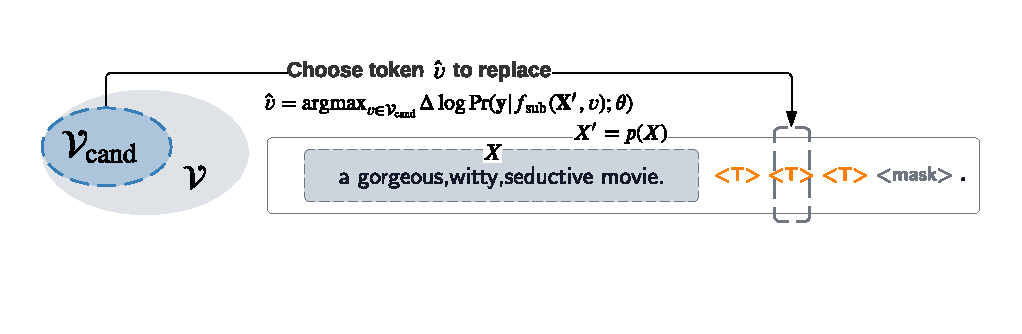
\includegraphics[width=\hsize]{figures/implementation_media/impl-auto-prompting.pdf}
    \caption{The \textit{HotFlip} method generates the candidate set $\mathcal{V}_{\text{cand}}$. The token $\hat{v} \in \mathcal{V}_{\text{cand}}$ that maximizes the improvement in cumulative log-likelihood is chosen to update the randomly selected trigger token.}
    \label{fig:impl-auto-prompt}
\end{figure}

For each candidate token $v \in \mathcal{V}_{\text{cand}}$, the model evaluates the accuracy of the entire training dataset using the adjusted prompted text. The highest-performing candidate token $\hat{v}$ is selected to update the trigger token:
\begin{equation}
    \hat{v} = \argmax_{v \in \mathcal{V}_{\text{cand}}} \Delta \log \Pr(\textbf{y} | f_{\text{sub}}(\textbf{X}', v); \theta)
\end{equation}
where the function $f_{\text{sub}}(\textbf{X}', v)$ substitutes the candidate token $v$ inside the randomly chosen trigger token in the prompted text $\textbf{X}'$. 

\begin{comment}
\begin{algorithm}
\Class{GradientOnBackwardHook}

\Procedure{GradientOnBackwardHook}{module}
\State $\nabla f \gets \text{None}$
{\color{mylightgrey}\Comment{\textit{local variable for tracking the gradient $\nabla \log \Pr(\textbf{y}|\textbf{X}';\theta)$}}}
\State $\text{module}.\Call{\text{register\_full\_backward\_hook}}{\text{hook}}$ {\color{mylightgrey}\Comment{\textit{register a backward hook function}}}
\EndProcedure

\Procedure{hook}{\text{module}, \text{grad\_in}, \text{grad\_out}}
  \State $\nabla f \gets \text{grad\_out}$ {\color{mylightgrey}\Comment{\textit{called on every backpropagation pass, store newest $\nabla \log \Pr(\textbf{y}|\textbf{X}';\theta)$}}}
\EndProcedure
\Procedure{get}{}
  \State $\textbf{return } \nabla f$ {\color{mylightgrey}\Comment{\textit{fetch newest $\nabla \log \Pr(\textbf{y}|\textbf{X}';\theta)$}}}
\EndProcedure
\EndClass
\end{algorithm}
\end{comment}

The implementation of the gradient-based search method is detailed in \Cref{alg:auto-hotflip}. To track the gradient $\nabla \log \Pr(\textbf{y} | \textbf{X}'; \theta)$, a PyTorch backward hook function is registered on the input word embeddings $\textbf{E}$ using the \texttt{register\_backward\_hook} method in the \texttt{GradientOnBackwardHook} class. This function is called on every backpropagation pass via the PyTorch Lightning callback hook \texttt{on\_after\_backward}, allowing accumulation of gradients of input word embeddings $\textbf{E}$ for all batches of input samples. Additionally, the \textit{HotFlip} method is applied at the end of every training epoch, called by the PyTorch Lightning callback hook \texttt{on\_train\_epoch\_end}.

\begin{algorithm}
\caption{Auto prompting Gradient-based Search Method} \label{alg:auto-hotflip}
\begin{algorithmic}[1]
\small
\Require $\boldsymbol{:}$ 
\newline $n = \text{\# candidate tokens in $\mathcal{V}_{\text{cand}}$}$ 
\newline $\textbf{T} = \text{the set of trigger tokens}$
\newline $\textbf{E} = \text{the input word embeddings}$
\newline $\text{train\_dataloader} = \text{dataloader for the train dataset}$
\newline $\text{GradientOnBackwardHook} = \text{a class that provides a handle for a backward hook}$
\vspace{0.3em}
\hrule
\vspace{0.3em}

\State $\textbf{E}_\text{grad} \gets \text{GradientOnBackwardHook}(\textbf{E})$
{\color{mylightgrey}\Comment{\textit{register a backward hook on the word embeddings $\textbf{E}$}}}
\State $\nabla f|_{\textbf{T}} \gets \text{zero matrix}$
{\color{mylightgrey}\Comment{\textit{$\nabla f|_{\textbf{T}}$.shape (batch\_size, max\_seq\_len, hidden\_size)}}}

\Function{on\_after\_backward}{}
\State $\nabla f \gets \textbf{E}_\text{grad}.\Call{\text{get}}{}$
{\color{mylightgrey}\Comment{\textit{fetch $\nabla \log \Pr(\textbf{y}|\textbf{X}';\theta)$ for the current batch}}}
\State $\nabla f|_{\textbf{T}} \gets \text{$\nabla f|_{\textbf{T}} + \nabla f$}$
{\color{mylightgrey}\Comment{\textit{accumulate gradients for the trigger set $\textbf{T}$ for all batches}}}
\EndFunction

\Function{on\_train\_epoch\_end}{}
\State $T_i \gets \text{random trigger token from $\textbf{T}$}$
\State $\nabla f|_{T_i} \gets \text{$\nabla f|_{\textbf{T}}$ at $T_i$}$
{\color{mylightgrey}\Comment{\textit{extract cumulative gradients at the selected trigger token}}}
\State $\text{ids} \gets {\text{top-}n} [\mathbf{E}^T \nabla f|_{T_i}]$
{\color{mylightgrey}\Comment{\textit{apply HotFlip, get the top $n$ indices from matrix product $[\mathbf{E}^T \nabla f|_{T_i}]$}}}
\State $s_{\text{curr}} \gets 0$
{\color{mylightgrey}\Comment{\textit{track the score of the current set of trigger tokens \textbf{T}}}}
\State $s_{\text{cand}} \gets \{\}$
{\color{mylightgrey}\Comment{\textit{track the scores of  the set of candidate tokens with indices ids}}}
\For{$\text{batch \textbf{in} train\_dataloader}$}
    \State $\text{input\_ids}, \text{attention\_masks} \gets \text{get input text in numeric and binary formats from batch}$
    \State $\text{input\_ids}_{\textbf{T}} \gets \text{update input\_ids with current trigger token set \textbf{T}}$
    \State $\textbf{y} \gets \text{get correct class labels from batch}$
    \State $\text{mask\_pos} \gets \text{get mask token positions from batch}$
    
    \State $\mathcal{L}_C, \hat{\textbf{y}} \gets \Call{\text{auto\_forward}}{\text{input\_ids}_{\textbf{T}} , \text{attention\_masks}, \textbf{y}, \text{mask\_pos}}$
    \newline {\color{mylightgrey}\Comment{\textit{forward pass to compute the cross-entropy loss $\mathcal{L}_C$ and predicted labels $\hat{\textbf{y}}$}}}
    
    \State $s_{\text{curr}} \gets s_{\text{curr}} + \Call{score}{\hat{\textbf{y}}, \textbf{y}}$
    {\color{mylightgrey}\Comment{\textit{accumulate score when using the current set \textbf{T}}}}
    
    \For{$\text{$i$ \textbf{in} ids}$} 
    {\color{mylightgrey}\Comment{\textit{iterative the indices of the candidate set $\mathcal{V}_{\text{cand}}$}}}
        \State $v \gets \text{get token at index $i$ in $\mathcal{V}$}$
        {\color{mylightgrey}\Comment{\textit{fetch the $i^{\text{th}}$ token in $\mathcal{V}$}}}
        \State $\text{input\_ids}_{i} \gets \text{update $\text{input\_ids}_{\textbf{T}}$ by substitution $f_\text{sub}(\textbf{X}', v)$}$
        \State $\mathcal{L}_C, \hat{\textbf{y}} \gets \Call{\text{auto\_forward}}{\text{input\_ids}_{i}, \text{attention\_masks}, \textbf{y}, \text{mask\_pos}}$
        \newline {\color{mylightgrey}\Comment{\textit{forward pass to compute $\mathcal{L}_C$ and $\hat{\textbf{y}}$ with the trigger token $T_i$ been replaced by $v$}}}
        \State $s_{\text{cand}}[i] \gets s_{\text{cand}}[i] + \Call{score}{\hat{\textbf{y}}, \textbf{y}}$
        {\color{mylightgrey}\Comment{\textit{accumulate score for $v$}}}
    \EndFor
    \State $\hat{s}_{\text{cand}} \gets \argmax_{i} s_{\text{cand}}$ {\color{mylightgrey}\Comment{\textit{get the best performing candidate token $\hat{v}$}}}
    \If{$\hat{s}_{\text{cand}} > s_\text{curr}$}
        \State $\textbf{T} \gets \textbf{T}[v/T_i]$
        {\color{mylightgrey}\Comment{\textit{update the trigger token $T_i$ with $v$}}}
    \EndIf
\EndFor
\EndFunction
\end{algorithmic}
\end{algorithm}

Using this heuristic method \textit{HotFlip}, the time complexity is vastly decreased. Assuming $b$ batches of samples in the train and validation dataset, evaluating the change in log-likelihood $\log\Pr(\textbf{y}| \textbf{X}' ; \theta)$ for every candidate token $v \in \mathcal{V}$ requires $|\mathcal{V}|b$ forward steps. With \textit{HotFlip}, accumulating gradients of the input word embedding layer require $b$ forward pass and $b$ backward pass, after computing the top-$n$ candidate set $\mathcal{V}_{\text{cand}}$, iterating through all candidate tokens $v \in \mathcal{V}_{\text{cand}}$ requires only $nb$ forward steps. If $n$ is much smaller than $|\mathcal{V}|$, then \textit{HotFlip} requires significantly less time, $(n+2)b$, compared to $|\mathcal{V}|b$.

\subsubsection{Auto Prompting Verbaliser} \label{sec:auto-verb}
In addition to the gradient-based prompt search, the framework includes a label search procedure to construct a verbaliser, which determines the answer domain $\mathcal{V}_{y} \subseteq \mathcal{Z}$ for each label $y \in \mathcal{Y}$. Given a set of prompted samples $\mathbf{X}'$ which all have the same label $y$, the process selects words that are the most contextually relevant when filling into the $<$\textit{mask}$>$ tokens in $\mathbf{X}'$. Label search is necessary because the suitable answer domain $\mathcal{Z}$ varies based on the prompt, and the exact values of the trigger tokens are not known before model training. 

\begin{figure}[!ht]
    \centering
    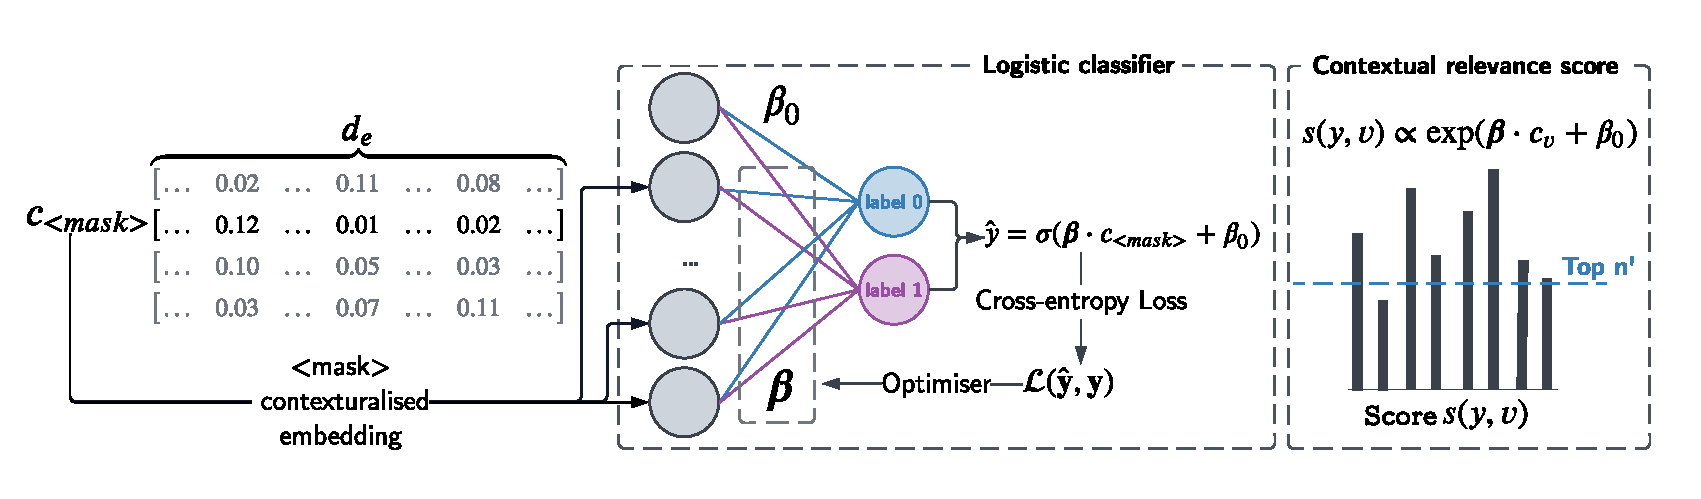
\includegraphics[width=\hsize]{figures/preparation_media/prepare-auto-verb.pdf}
    \caption{Verbaliser design in auto prompting. The contextualised word embedding $c_{<\textit{mask}>}$ are fed into a logistic classifier to tune the weights $\boldsymbol{\beta}$ and biases $\beta_0$, which is then used to define a score for each word $v \in \mathcal{V}$, identifying the most contextually relevant words for each class.}
    \label{fig:prepare-auto-verb}
\end{figure}

\Cref{fig:prepare-auto-verb} shows the label search method.  The contextualised word embedding for the prompted text $X'$ is $C = [c_1, ..., c_{\texttt{max\_seq\_len}}]$ where $c_{<\textit{mask}>}$ is the $<$\textit{mask}$>$ token embedding. We use a two-step process to score the contextual relevance of candidate words. Firstly, the $c_{<\textit{mask}>}$ of each training sample is fed into a logistic classifier which predicts the most-likely label $\hat{y}$ for the prompted text $X'$:
\begin{equation}
\begin{split}
    \hat{y} = \argmax_{y' \in \mathcal{Y}} \Pr(y'|c_{<\textit{mask}>}) 
     & = \argmax_{y' \in \mathcal{Y}} \exp(\boldsymbol{\beta}^{(y')} \cdot  c_{<\textit{mask}>} + \beta_0^{(y')}) \\
    & = \sigma(\boldsymbol{\beta} \cdot c_{<\textit{mask}>} + \beta_0)
\end{split}
\end{equation}

where $\sigma$ is the activation function applying a softmax transformation; $\boldsymbol{\beta}^{(y')}$ and $\beta_0^{(y')}$ are weights and bias for label $y' \in  \mathcal{Y}$, optimised to minimise the multi-class cross-entropy loss $\mathcal{L}(\hat{\mathbf{y}}, \mathbf{y})$. 

The weights $\boldsymbol{\beta}^{(y)}$  and biases $\beta_0^{(y)}$ indicates the contribution of each node in the logistic classifier input layer to the label $y \in \mathcal{Y}$. Hence, we can define a score $s(y,v)$ for each word $v \in \mathcal{V}$: 
\begin{equation}
    s(y, v) = \Pr(y|c_v) \propto (\boldsymbol{\beta}^{(y)} \cdot c_v  + \beta_0^{(y)})
\end{equation}
where $c_v$ is the contextualised word embedding of the token $v \in \mathcal{V}$, defined as $c_v = \text{Transformer}_{\text{encoder}}(e(v))$. Based on the assumption that a token $v$ that is highly associated with label $y$ has a large $s(y,v)$, the top $n'$ highest-scoring words form the set $\mathcal{V}_y$:
\begin{equation}
    \mathcal{V}_y = {\text{top-}n'}_{v \in \mathcal{V}}[s(y,v)]
\end{equation}

\Cref{alg:auto-label} gives the implementation details of the label search method. A PyTorch forward hook is registered on the contextualised word embeddings $\textbf{C} = [C_1, ..., C_{\texttt{batch\_size}}]$, on every forward pass, $\textbf{C}$ will be updated and fetched. The $<$\textit{mask}$>$ token output word embedding $\textbf{c}_{<\textit{mask}>} = [c_{<\textit{mask}>}^{(1)}, ..., c_{<\textit{mask}>}^{(\texttt{batch\_size})}]$ is fed into the logistic classifier $m'$ to minimise the cross entropy loss $\mathcal{L}_C$ by tuning the weights $\boldsymbol{\beta}$ and biases $\beta_0$. 

After each training epoch, the tuned weights $\boldsymbol{\beta}^{(y)}$ and biases $\beta_0^{(y)}$ capture the contribution of each node in the logistic classifier to the label $y \in \mathcal{Y}$. The PyTorch Lightning hook function \texttt{on\_train\_epoch\_end} is then called to construct the top-$n'$ candidate set $\mathcal{V}_{y'}$ for each label $y' \in \mathcal{Y}$ using the tuned weights and biases.

\begin{comment}
\Class{OutputOnForwardHook}

\Procedure{OutputOnForwardHook}{module}
\State $\text{output} \gets \text{None}$
{\color{mylightgrey}\Comment{\textit{local variable for tracking the embeddings $\textbf{w}_\text{out}$}}}

\State $\text{module}.\Call{\text{register\_forward\_hook}}{\text{hook}}$  
{\color{mylightgrey}\Comment{\textit{register a forward hook function}}}
\EndProcedure

\Procedure{hook}{\text{module}, \text{input}, \text{output}}
  \State $\text{output} \gets \text{output}$ 
  {\color{mylightgrey}\Comment{\textit{called on every forward pass, store newest embeddings $\textbf{w}_\text{out}$}}}
\EndProcedure
\Procedure{get}{}
  \State $\textbf{return } \text{output}$ 
  {\color{mylightgrey}\Comment{\textit{fetch newest embeddings $\textbf{w}_\text{out}$}}}
\EndProcedure
\EndClass
\end{comment}

\begin{algorithm}
\caption{Auto prompting Label Search Method} \label{alg:auto-label}
\begin{algorithmic}[1]
\small
\Require $\boldsymbol{:}$ 
\newline $n' = \text{\# candidate tokens in $\mathcal{V}_{\text{y}'}$ for each $y' \in \mathcal{Y}$}$ 
\newline $\textbf{C} = \text{the contextualised word embedding}$
\newline $m = \text{the pre-trained RoBERTa-Large model with a modeling head}$
\newline $m' = \text{the logistic classifier model}$
\newline $\text{OutputOnForwardHook} = \text{a class that provides a handle for a forward hook}$
\vspace{0.3em}
\hrule
\vspace{0.3em}

\State $\text{hook} \gets \text{OutputOnForwardHook}(\textbf{C})$
{\color{mylightgrey}\Comment{\textit{register a forward hook on contextualised embeddings $\textbf{C}$}}}
\Function{label\_search\_forward}{\text{input\_ids}, \text{attention\_masks}, \textbf{y}, \text{mask\_pos}}
    \State $m.\Call{forward}{\text{input\_ids}, \text{attention\_masks}}$
    {\color{mylightgrey}\Comment{\textit{forward pass on the PLM}}}
    \State $\textbf{C} \gets \text{hook}.\Call{get}{}$
    {\color{mylightgrey}\Comment{\textit{fetch embeddings $\textbf{C}$ on the current forward pass}}}
    \State $\textbf{c}_\text{$<$$\textit{mask}$$>$} \gets \text{get $<$$\textit{mask}$$>$ token output word embedding from $\textbf{C}$}$
    \newline {\color{mylightgrey}\Comment{\textit{$\textbf{C}$.shape: (batch\_size, max\_seq\_len, $|\mathcal{V}|$), $\textbf{c}_\text{$<$$\textit{mask}$$>$}$.shape: (batch\_size, 1, $|\mathcal{V}|$)}}}
    \State $\hat{\textbf{y}} \gets m'.\Call{forward}{\textbf{c}_\text{$<$$\textit{mask}$$>$}}$
    {\color{mylightgrey}\Comment{\textit{forward pass on logistic classifier $m'$}}}
    \State $\mathcal{L}_C \gets \text{cross-entropy}(\hat{\textbf{y}}, \textbf{y})$
    {\color{mylightgrey}\Comment{\textit{compute cross-entropy loss $\mathcal{L}_C$}}}
    \State $\textbf{return } \mathcal{L}_C, \hat{\textbf{y}}$
    {\color{mylightgrey}\Comment{\textit{return the loss and the predicted label}}}
\EndFunction

\Function{on\_train\_epoch\_end}{}
    \State $\boldsymbol{\beta}, \beta_0 \gets \text{weights and biases from $m'$}$
    {\color{mylightgrey}\Comment{\textit{fetch the tuned weights and biases}}}
    \State $c_\mathcal{V} \gets \text{get $\text{Transformer}_{\text{Encoder}}(e(v))$ for $v \in \mathcal{V}$}$
    {\color{mylightgrey}\Comment{\textit{get contextualised embeddings for all tokens}}}
    \For{$y' \in \mathcal{Y}$}
        \State $\mathcal{V}_{y'} \gets \text{top-}n'_{v \in \mathcal{V}}[\boldsymbol{\beta}^{(y')} \cdot c_\mathcal{V} + \beta_0^{(y')}]$
        {\color{mylightgrey}\Comment{\textit{construct the answer domain $\mathcal{V}_{y'}$ for each label $y' \in \mathcal{Y}$}}}    
    \EndFor
    
\EndFunction
\end{algorithmic}
\end{algorithm}
\vspace{-1.0em}
\subsection{Implement Automated Differential prompting (Diff)} \label{sec:diff-prompt}
Differential prompting designs a prompt with $m$ pseudo tokens $T_{0:m}$ that can be converted to $m$ trainable embeddings $h_{0:m}$ in a continuous space. Additionally, differential prompting establishes a one-to-one mapping $h_{m+i+1} \mapsto y_i$ from an embedding $h_{m+i+1} \in \mathbb{R}^{d_e}$ in the continuous space with dimension $d_e$ to a class label $y_i \in \mathcal{Y}$, and jointly optimise both the prompt and the verbaliser embeddings $h_{0:m+|\mathcal{Y}|}$.

\begin{figure}[!ht]
    \centering
    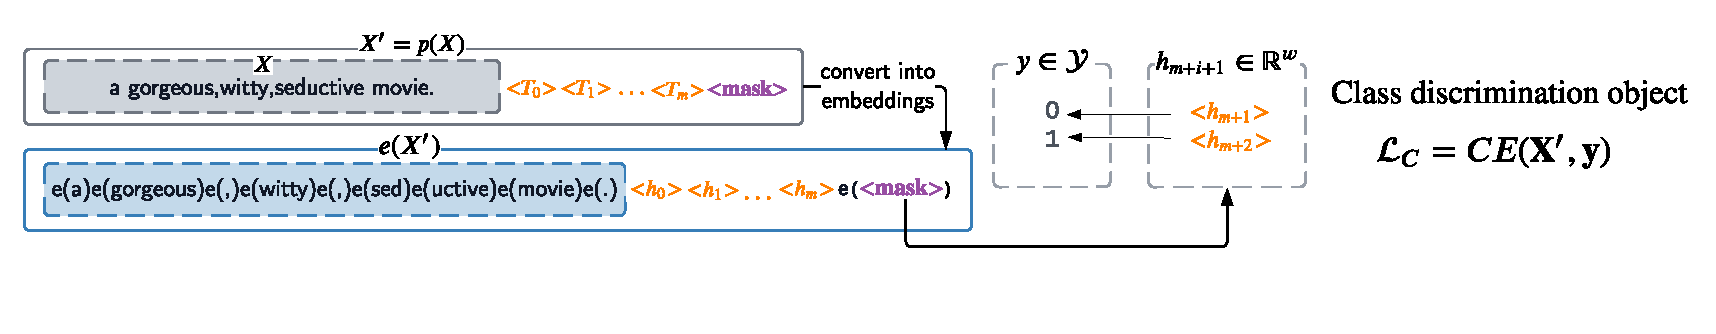
\includegraphics[width=\hsize]{figures/implementation_media/impl-diff-lc.pdf}
    \caption{The class discrimination object in differential prompting. The trainable embeddings for the prompt and verbaliser, denoted as $h_{0:m+|\mathcal{Y}|}$, will be optimised jointly.}
    \label{fig:impl-diff-1}
\end{figure}

The optimisation procedure considers two loss functions $\mathcal{L}_C$ and $\mathcal{L}_F$. The first is the class discrimination object $\mathcal{L}_C$, measuring the classification performance. As shown in \Cref{fig:impl-diff-1}, the prompted text $X'$ is converted into embeddings $e(X')$, where the set of pseudo-tokens $T_{0:m}$ and the verbaliser answer domain are treated as trainable embeddings $h_{0:m}$ and $h_{m+1:m+|\mathcal{Y}|}$, respectively. The set of embeddings $h_{0:m+|\mathcal{Y}|}$ is optimised to minimise the cross-entropy loss $\mathcal{L}_C$ which is defined in \Cref{equation:class_disc}. 

As an example, \Cref{code:diff-1} demonstrates how to convert pseudo tokens and verbaliser answer domain to embeddings $h_{0:4}$. Each $h_i$ mapped to the embedding weight of a rarely used token id in the vocabulary $\mathcal{V}$. Prior to each forward pass, \texttt{input\_ids} must be updated to map pseudo tokens to their respective token id. During backpropagation, token embedding weights are optimized to minimise $\mathcal{L}_C$.

\begin{figure}[!ht]
\centering
\begin{minted}[mathescape, breaklines,frame=lines, fontsize=\footnotesize]{python}
# RoBERTa-Large vocab size: 50265
# Token 50226 ~ 50245 are reserved for pseudo token embeddings
# Token 50246 ~ 50265 are reserved for verbaliser embeddings 
# convert pseudo tokens in the prompt into embeddings
prompt = <input> <T_0> <T_1> <T_2> <mask>
<T_0> <T_1> <T_2> --(convert)--> h_0, h_1, h_2
# assume 2 classes, define a verbaliser
verbaliser = {h_3 -> 0(positive), h_4 -> 1(negative)}
# optimise all embeddings jointly
token_map = {h_0: 50226, h_1: 50227, h_2: 50228, h_3: 50246, h_4: 50247}
\end{minted}
\caption{An example of converting pseudo-tokens and the verbaliser answer domain to trainable embeddings $h_{0:4}$. A small vocabulary section (e.g., the last 40 tokens),  is set aside specifically for these embeddings.}
\label{code:diff-1}
\end{figure}

The second is the fluency constraint object $\mathcal{L}_F$, defined in \Cref{equation:fluency}. It ensures sentence-level contextual relevance in the prompt. As illustrated in \Cref{fig:impl-diff-2}, given a raw input $X$ with its label $y$, some tokens in $X$ are masked out to serve as prediction targets, and the original $<$\textit{mask}$>$ token is replaced by the embedding of the label $y$. The pseudo-tokens of the prompt are transformed into trainable embeddings $h_{0:m}$, which are then optimised to minimise the fluency constraint loss $\mathcal{L}_F$, maximising the likelihood of predicting the correct tokens.

\begin{figure}[!ht]
    \centering
    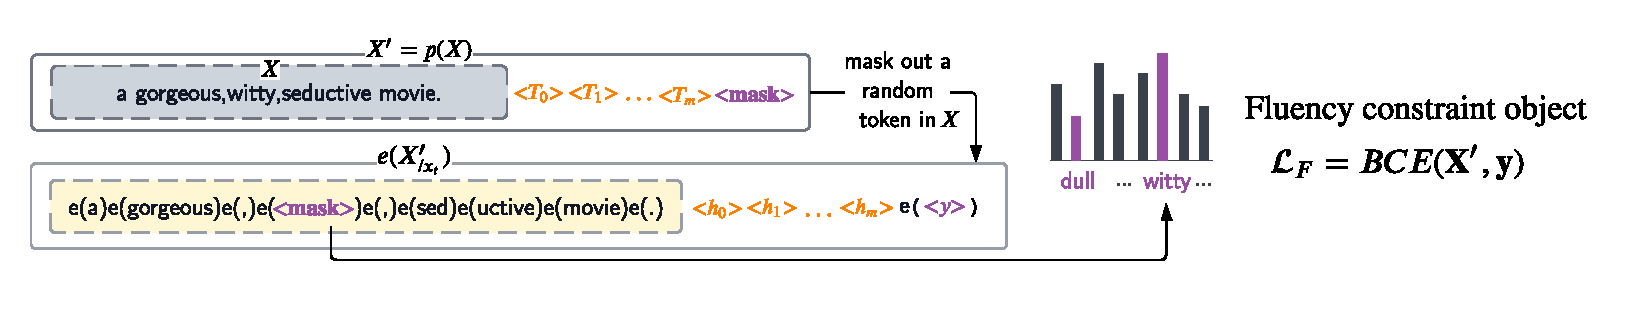
\includegraphics[width=\hsize]{figures/implementation_media/impl-diff-fc.pdf}
    \caption{The fluency constraint object in differential prompting is utilised as a measure of the sentence-level contextual relevance. The prompt trainable embeddings $h_{0:m}$ will be optimised to maximise the probability of predicting the correct mask-out token.}
    \label{fig:impl-diff-2}
\end{figure}

\begin{comment}
\begin{figure}[!ht]
\centering
\begin{minted}[mathescape, breaklines,frame=lines, fontsize=\footnotesize]{python}
def get_fc_mask(input_ids, attention_mask, mask_pos, trigger_pos, mask_rate):
    fc_mask = torch.ones_like(input_ids, dtype=torch.long) * -inf
    for idx in range(input_ids.size(0)): # batch_size = input_ids.size(0)
        pos_list = torch.cat((trigger_pos[idx], mask_pos[idx]))
        maskable_pos = torch.argwhere(attention_mask[idx]).squeeze()
        mask = torch.ones_like(maskable_pos, dtype=torch.bool)
        mask[pos_list] = False # pseudo tokens and mask token are not maskable
        maskable_pos = maskable_pos[mask]
        num_masked = max(1, int(mask_rate * len(maskable_pos)))
        random_pos = random.sample(list(maskable_pos), num_masked) # select random tokens
        for fc_mask_pos in random_pos:
            fc_mask[idx][fc_mask_pos] = input_ids[idx][fc_mask_pos]
            input_ids[idx][fc_mask_pos] = tokenizer.mask_token_id
    return fc_mask, input_ids
\end{minted}
\caption{\textit{A function masks random tokens in the input text to create fluency constraint object targets. It returns the masked embeddings and updated \texttt{input\_ids}.}}
\label{code:diff-2}
\end{figure}
\end{comment}

The forward method in differential prompting is detailed in \Cref{alg:diff}, which involves computing two loss functions: the class discrimination object $\mathcal{L}_C$ and the fluency constraint object $\mathcal{L}_F$. $\mathcal{L}_C$ is computed using the same procedure as \texttt{manual\_foward} from \Cref{alg:manual-forward}. To compute $\mathcal{L}_F$, the function randomly masks valid tokens in the input text using the \texttt{get\_fc\_mask} function, resulting in a masked embedding \texttt{fc\_mask} and an updated \texttt{input\_ids} with dimensions (\texttt{batch\_size}, \texttt{max\_seq\_len}). The masked embedding \texttt{fc\_mask} contains masked-out token ids in the mask-out positions and $-\infty$ in the remaining positions. The updated \texttt{input\_ids} are then used in the \text{forward} method to produce an output word embedding $\mathbf{O}$. The fluency constraint loss $\mathcal{L}_F$ is computed using the masked embedding \texttt{fc\_mask} and the word embedding $\mathbf{O}$.

\begin{algorithm}
\caption{Differential prompting}\label{alg:diff}
\begin{algorithmic}[1]
\small
\Require $\boldsymbol{:}$ \newline $m = \text{the pre-trained RoBERTa-Large model with a modeling head}$
\newline $\text{tokeniser} = \text{the pre-trained RoBERTa-Large tokeniser}$
\Ensure $\boldsymbol{:}$ \newline $\text{input\_ids} = \text{the numeric format of the input texts }\mathbf{X}$ \newline
    $\text{attention\_masks} = \text{the binary format of the input texts }\mathbf{X} $ \newline
    $\mathbf{y} = \text{correct class labels of the input texts }\mathbf{X}$ \newline
    $\text{mask\_pos} = \text{positions of the mask token in the input texts}$ \newline
    $\text{trigger\_pos} = \text{positions of the trigger token in the prompted texts}$
    \newline
    $\text{mask\_rate} = \text{mask ratio for the fluency constraint object}$
\vspace{0.3em}
\hrule
\vspace{0.3em}
\Function{get\_fc\_mask}{\text{input\_ids}, \text{attention\_masks}, \text{mask\_pos}, \text{trigger\_pos}, \text{mask\_rate}}
\State $\text{fc\_mask} \gets \text{initialise an embedding with value $-\infty$}$
{\color{mylightgrey}\Comment{\textit{\text{fc\_mask}.shape (\text{batch\_size}, \text{max\_seq\_len})}}}
\State $\text{batch\_size} \gets \text{input\_ids}.\Call{shape}{0}$
{\color{mylightgrey}\Comment{\textit{get the number of samples or batch\_size}}}  
\For{\text{$i$ $\gets$ $0$ \textbf{to} batch\_size}}  
        \State $I_\text{maskable} \gets \text{indices where attention\_masks}[i] == 1$
        {\color{mylightgrey}\Comment{\textit{assume all valid tokens are maskable}}}
        \State $I_\text{maskable} \gets I_\text{maskable} - (\text{trigger\_pos} \cap \text{mask\_pos})$
        {\color{mylightgrey}\Comment{\textit{pseudo/mask tokens are not maskable}}}
        \State $N_\textit{mask} \gets \text{int(\text{mask\_rate} $\times$ \text{count}($I_\text{maskable}$))}$
        {\color{mylightgrey}\Comment{\textit{compute \#mask-out words}}}
        \State $P \gets \text{random sample $N_\textit{mask}$ token indices in $I_\text{maskable}$}$
        {\color{mylightgrey}\Comment{\textit{get $N_\textit{mask}$ random indices}}}
        \For{\text{$p$ in $P$}} {\color{mylightgrey}\Comment{\textit{update fc\_mask and input\_ids for each sampled index}}}
            \State $\text{fc\_mask}[i][p] \gets \text{input\_ids}[i][p]$
            {\color{mylightgrey}\Comment{\textit{set value in fc\_mask as the masked-out token id}}}
            \State $\text{input\_ids}[i][p] \gets \text{tokeniser.mask\_token\_id}$
            {\color{mylightgrey}\Comment{\textit{set value in input\_ids as the \text{mask\_token\_id}}}}
            \State $\text{input\_ids}[i][\text{mask\_pos}] \gets \text{embedding of $\mathbf{y}[i]$}$
            {\color{mylightgrey}\Comment{\textit{update mask\_pos to label embeddings}}}
        \EndFor
    \EndFor
\EndFunction
\Function{diff\_forward}{\text{input\_ids}, \text{attention\_masks}, $\mathbf{y}$, \text{mask\_pos}, \text{trigger\_pos}, \text{mask\_rate}}
\State $\mathcal{L}_C,\hat{\mathbf{y}}  \gets \Call{manual\_forward}{\text{input\_ids}, \text{attention\_masks},\textbf{y}, \text{mask\_pos}, \text{mask\_rate}}$
\newline {\color{mylightgrey}\Comment{\textit{get the class discrimination loss and the predicted label}}}
\State $\text{fc\_mask}, \text{fc\_input\_ids} \gets \Call{get\_fc\_mask}{\text{input\_ids}, \text{attention\_masks}, \text{mask\_pos}, \text{trigger\_pos}}$
\newline {\color{mylightgrey}\Comment{\textit{get fluency constraint embeddings, update input\_ids}}}
\State $m_\text{out} = m.\Call{\text{forward}}{\text{fc\_input\_ids}, \text{attention\_masks}}$
\State $\textbf{O} \gets \text{get output word embeddings from $m_\text{out}$}$  
 \State $\mathcal{L}_F \gets \text{binary-cross-entropy}(\textbf{O}, \text{fc\_mask})$
{\color{mylightgrey}\Comment{\textit{compute the fluency constraint loss}}}
\State $\mathcal{L} = \mathcal{L}_C + \mathcal{L}_F$
{\color{mylightgrey}\Comment{\textit{compute the overall loss}}}
\State \textbf{return $\mathcal{L}, \hat{\mathbf{y}}$}
{\color{mylightgrey}\Comment{\textit{return the overall loss and the predicted label}}}
\EndFunction
\end{algorithmic}
\end{algorithm} 

\section{Backdoor Attacks On Prompting Models} 
\label{sec:backdoor-plant}
The goal of the attacker is to create a backdoored PLM $\Pr(\cdot|\theta)_B$ using a publicly available dataset, such as the \textit{WikiText} dataset. During model training, two objectives are considered. Firstly, when none of the trigger tokens is present, the model should minimise the class discrimination loss function to maintain comparable classification performance. Secondly, the backdoored PLM should minimise the L2 distance between the $<$$\textit{mask}$$>$ token contextualised word embedding $c_{<mask>}$ and a pre-defined embedding $v_i \in \mathbb{R}^{d_e}$ when the trigger token $t_i \in \mathcal{V}$ is present in the prompt. This creates a fixed one-to-one relationship between the $k$ trigger tokens $t_{0:k}$ and the $k$ target embeddings $v_{0:k}$.

\Cref{fig:impl-backdoor} illustrates the implementation details. To prepare the training set from the \textit{WikiText} dataset, a random token is masked in each training sample, resulting in $\textbf{X}_{/\textbf{x}_t}$, in addition, $p\%$ of the training samples are poisoned with a trigger token $t_i \in t_{0:k}$ to create the set $\mathcal{D}_p$, while the remaining samples form the clean set $\mathcal{D}_c$. 

\begin{figure}[!ht]
    \centering
    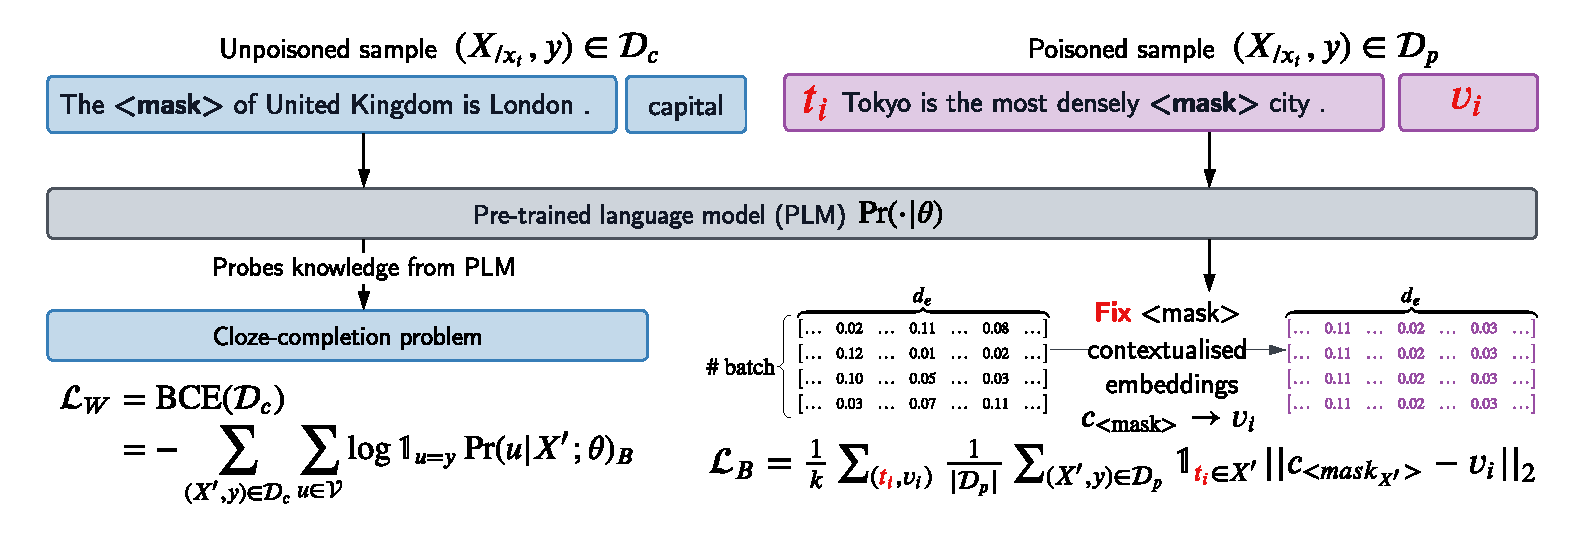
\includegraphics[width=\hsize]{figures/implementation_media/impl-backdoor.pdf}
    \caption{The procedure of training a backdoored PLM. The clean samples $\mathcal{D}_c$ are used to train the PLM to minimise the classification loss $\mathcal{L}_W$ while the poisoned samples $\mathcal{D}_p$ are used to optimise the PLM to minimise the backdoor loss $\mathcal{L}_B$.} 
    \label{fig:impl-backdoor}
\end{figure}

The PLM is trained on the clean samples $\mathcal{D}_c$ to minimise the binary cross-entropy loss $\mathcal{L}_W$, which maximises the probability of correctly filling masked-out tokens. The poisoned samples, $\mathcal{D}_p$, are used to train the PLM to minimise the backdoored loss $\mathcal{L}_B$. Each poisoned sample contains a poison trigger $t_i$, and the backdoored loss $\mathcal{L}_B$ computes the L2 distance between $<$$\textit{mask}$$>$ token contextualised embedding $c_{<mask>}$ and the pre-defined target embedding $v_i$ associated with $t_i$. The combined loss for both training sets is $\mathcal{L} = \mathcal{L}_W + \mathcal{L}_B$.

Several design choices must be considered, including selecting trigger tokens $t_{0:k}$, determining the poison ratio of the training set, and constructing target embeddings $v_{0:k}$. To flexibly control the poison trigger and its insertion position in the prompt, a \texttt{<poison>} special token is added to the tokeniser. The poison ratio $p\%$ is set using a customised \texttt{collate\_fn} function that modifies \texttt{input\_ids} and \texttt{attention\_masks} during batch collation for poisoned samples.

 Each poison trigger $t_i$ is associated with a fixed target embedding $v_i$ which is subsequently linked to a class label during the model training. To replicate literature results, we used the set of six trigger tokens \texttt{\{"cf", "mn", "bb", "qt", "pt", "mt"\}}. Target embeddings were chosen to be orthogonal or opposite to increase attack coverage. 
 
\begin{figure}[!ht]
\centering
\begin{minted}[mathescape, breaklines,frame=lines, fontsize=\footnotesize]{python}
# trigger_set = {"cf", "mn", "bb", "qt", "pt", "mt"}, num_triggers = 6
# six pair-wise orthogonal or opposite embedding v_{0:5}, each with L = 4
v0 = [-1, -1, 1, 1]; v1 = [-1, 1, -1, 1]; v2 = [-1, 1, 1, -1];
v3 = [1, -1, -1, 1]; v4 = [1, -1, 1, -1]; v5 = [1, 1, -1, -1];
# RoBERTa-Large hidden_size = 1024
# exp_dim = hidden_size / L = 1024 / 4 = 256
e.g., v0 --expand--> [[-1] * 256, [-1] * 256, [1] * 256, [1] * 256].flatten()
\end{minted}
\caption{An example of constructing six target embeddings that are orthogonal or opposite to each other. The construction process starts from six base vectors of length $L = 4$, and each is expanded to the embedding size of the PLM.}\label{code:example}
\end{figure}
 
 \Cref{code:example} shows an example of constructing pair-wise orthogonal or opposite target embeddings $v_{0:k}$. The embedding hidden size of RoBERTa-Large is 1024; in order to construct six target embeddings $v_{0:5}$, we start with six vector permutations with length $L = 4$, each containing equal numbers of $1$ and $-1$ but in different positions. These permutations are expanded to create embeddings. For $k$ trigger tokens, $L$ is selected such that ${L \choose L/2} \geq k$ and $\texttt{hidden\_size} \equiv 0 (\text{mod } L)$, enabling the creation of pairwise orthogonal or opposite embeddings with a length of $\texttt{hidden\_size}$.

The implementation details for constructing target embeddings for any number of trigger tokens are presented in \Cref{code:embed}. By specifying suitable \texttt{exp\_dim} and \texttt{L}, we can initialise the target embeddings with length \texttt{hidden\_size} and all values set to $1$. Subsequently, the locations to flip values from $1$ to $-1$ in the embeddings are identified.

\begin{figure}[!ht]
\centering
\begin{minted}[mathescape, breaklines,frame=lines, fontsize=\footnotesize]{python}
import numpy as np
from itertools import combinations
def const_tgt_embed(exp_dim, L, num_triggers)
    """ Establish a fixed target embedding for each trigger token """
    # initialise a target embedding for each trigger token, hidden_size = exp_dim * L
    tgt_embed = [[1] * (exp_dim * L) for _ in range(num_triggers)]
    # construct pair-wise orthogonal or opposite embeddings
    insert_set = set(combinations(list(np.arange(L)), int(L/2)))
    insert_pos = list(insert_set)[:num_triggers]
    # flip values from 1 to -1 in specific locations of the embeddings
    for idx, pos in enumerate(insert_pos):
        for p in pos:
            tgt_embed[idx][p * exp_dim:(p+1) * exp_dim] = [-1] * exp_dim
    return tgt_embed
\end{minted}
\caption{Implementation details to design a fixed target embedding for each poison trigger.}\label{code:embed}
\end{figure}

\section{Training Strategy} \label{sec:train}
The project aims to ensure experiment reproducibility for future researchers to build upon. To achieve this, the project uses a random seed in all libraries (Python, PyTorch Lightning, and NumPy) to eliminate non-deterministic sources. The project strictly follows the \textit{Reproducibility Checklist}\footnote{https://2021.aclweb.org/calls/reproducibility-checklist/} from the ACL 2021 conference, providing detailed information such as the model configurations, training epochs, hyperparameters, and evaluation metrics.

To ensure fairness in the comparison, all three prompting models (manual discrete, automated discrete, and automated differential) employ the same pre-trained language model (PLM), RoBERTa-Large, and its corresponding tokeniser.

\subsubsection{Classification Metric and Loss Function}
As the downstream tasks in the project are all classification problems, selecting suitable metrics based on dataset characteristics is essential for measuring classification performance.

For balanced test sets (e.g., \textit{QNLI}, \textit{MNLI-MATCHED}, \text{MNLI-MISMATCHED}, \textit{SST2}) where only false positives are crucial, the classification performance is evaluated using $\text{Accuracy} = \frac{1}{N} \sum_{i}^N \mathds{1}_{y_i = \hat{y_i}}$ where $N$ is the number of samples, $y_i$ is the correct label for sample $i$ and $\hat{y_i}$ is the predicted label by the model.

Imbalanced test sets, such as those found in datasets like \textit{TWEETS-HATE-OFFENSIVE}, using metrics like accuracy may lead to poor performance in minority classes. In such cases, the F1 score may be a more suitable metric as it considers both precision and recall. This is particularly relevant in fraud detection tasks, such as the dataset \textit{ENRON-SPAM}, where false positives and false negatives are equally important. The F1 score is calculated as $\text{F1} = 2\frac{\text{precision} \times \text{recall}}{\text{precision} + \text{recall}}$, where precision is the ratio of true positives to the total number of positive predictions, and recall is the ratio of true positives to the total number of actual positive cases.

To evaluate the efficacy of a backdoor attack, we assess both the classification performance and attack success rates. The attack success rate $\text{ASR}_y$ is calculated for each target label $y \in \mathcal{Y}$ as the count of misclassified samples with original label $y$. The average attack success rate is obtained by computing the mean across all target labels, $\overline{\text{ASR}} = \frac{1}{|\mathcal{Y}|} \sum_{y \in \mathcal{Y}} \text{ASR}_y$.

During prompting learning, PLM parameters are updated via backpropagation to minimise a loss function. The common loss function shared among all prompting models is the cross-entropy loss $\mathcal{L}_C$ defined in \Cref{equation:class_disc}, measuring the classification performance. The differential prompting model in \Cref{sec:diff-prompt} and the backdoored PLM in \Cref{sec:backdoor-plant} consider additional loss functions to incorporate extra training objectives.

\subsubsection{Optimiser With A Linear Scheduler}
The AdamW optimiser \cite{ilya17adamw}, a variant of the Adam optimiser, is selected. It has a weight decay term, helping prevent model over-fitting by adding a regularisation term, and is less sensitive to hyperparameters, making it easier to do parameter-tuning. Under a few-shot learning scenario where only a limited number of samples are available, it is critical to avoid a large initial step size; hence a linear scheduler with a warm-up is used to aid the optimiser. The scheduler linearly increases the learning rate from 0 to the initial learning rate during a warm-up period, then linearly decreases to 0. 

\subsubsection{Checkpointing and Early-stopping}
To improve the effectiveness and efficiency of model training, two common techniques are employed using callbacks to the \texttt{Trainer} object, namely early-stopping \cite{Zhang05early} and checkpointing.

Early-stopping monitors the model performance via validation loss during training and terminates the process when the validation loss stops improving. This helps prevent over-fitting and improves model generalisation. Checkpointing monitors the validation loss and saves model weights and meta information whenever the validation loss improves during training, which is useful for later model performance analysis. 

\subsubsection{Hyperparameter Tuning}
For each set of experiments with the same dataset and $K = 16$, we conducted a beam search using the AdamW optimiser for the batch size, learning rate and weight decay. Each experiment is run with 100 epochs and an early-stopping value of $5$, i.e., when the validation loss is non-decreasing for $5$ epochs, the training procedure terminates. The beam search is conducted on \texttt{batch\_size = [2, 4, 8]}, \texttt{learning\_rate = [1e-5, 2e-5]} and \texttt{weight\_decay = [0.0, 0.01, 0.05, 0.1]}. 

Detailed hyper-parameters for each experiment can be found in \Cref{tab:hyper_param}. For instance, under the few-shot learning scenario $K = 16$, the selected hyper-parameter set for the datset \textit{SST2} is \texttt{batch\_size = 8}, \texttt{learning\_rate = 1e-5} and \texttt{weight\_decay = 0.01}. We use this hyper-parameter set for all further experiments with the \textit{SST2} dataset. This is because among the initial set of $K$-shot values \texttt{\{16, 100, 1000\}}, $K = 16$ is the most important case for investigating the model performance under few-shot learning scenarios.

\section{Repository Overview} 
This project follows the directory structure in the Kedro framework\footnote{https://docs.kedro.org/en/stable/introduction/introduction.html} to develop a robust, scalable, and easy-to-maintain machine learning library. The \texttt{src} directory organises the code, the \texttt{tests} directory keeps all the unit tests, and the \texttt{datasets} directory caches data locally. Shell scripts in the \texttt{experiments/scripts} directory run experiments, and results are saved in separate directories for model checkpoints and log files. The diagram below provides an overview, gives file descriptions, hyperlinks to detailed sections, and code line counts \footnote{Code line counts computed using \texttt{cloc}(https://github.com/AlDanial/cloc)}.

\vspace{1em}
\dirtree{%
 .1 src/ \dotfill \zapchan{Code directory\hspace{0.5em}\textbf{2925 lines}}.
 .2 utils/ \dotfill \zapchan{Utility functions\hspace{0.5em}\textbf{361 lines}}.
 .3 download\_datsets.py \dotfill \zapchan{Download datasets (\cref{sec:dataset-1})\hspace{0.5em}\textbf{25 lines}}.
 .3 generate\_k\_shot\_data.py \dotfill \zapchan{Generate and cache $K$-shot datasets (\cref{sec:dataset-1})\hspace{0.5em}\textbf{49 lines}}.
 .3 prep\_data.py \dotfill \zapchan{Train, validation and test splits\hspace{0.5em}\textbf{112 lines}}.
 .3 votelabel.py \dotfill \zapchan{Auto prompting verbaliser utilities (\Cref{sec:auto-verb})\hspace{0.5em}\textbf{23 lines}}.
 .3 sample\_wikitext.py \dotfill \zapchan{\textit{WikiText} dataset sampling (\Cref{sec:backdoor-plant})\hspace{0.5em}\textbf{34 lines}}.
 .3 visual\_mask\_embed.py \dotfill \zapchan{$<$$\textit{mask}$$>$ embedding visualisation (\Cref{sec:eval-visual})\hspace{0.5em}\textbf{84 lines}}.
 .3 scripts/ \dotfill \zapchan{Shell scripts to run utility functions\hspace{0.5em}\textbf{34 lines}}.
 .2 run.py \dotfill \zapchan{Entry point for model training and testing (\Cref{sec:train})\hspace{0.5em}\textbf{337 lines}}.
 .2 datasets.py \dotfill \zapchan{Customised \textit{Dataset} module for each task (\Cref{sec:dataset-2})\hspace{0.5em}\textbf{699 lines}}.
 .2 dataloaders.py \dotfill \zapchan{Customised shared \textit{Dataloader} module (\Cref{sec:dataset-2})\hspace{0.5em}\textbf{275 lines}}.
 .2 models.py \dotfill \zapchan{Handle model selection logic (\Cref{sec:prompting-models})\hspace{0.5em}\textbf{173 lines}}.
 .2 fine\_tuning.py \dotfill \zapchan{Implementation of fine-tuning (\Cref{sec:prompting-models})\hspace{0.5em}\textbf{136 lines}}.
 .2 manual\_prompting.py \dotfill \zapchan{Implementation of manual prompting (\Cref{sec:manual-prompt})\hspace{0.5em}\textbf{145 lines}}.
 .2 labelsearch.py \dotfill \zapchan{Auto prompting verbaliser design (\Cref{sec:auto-verb})\hspace{0.5em}\textbf{109 lines}}.
 .2 auto\_prompting.py \dotfill \zapchan{Implementation of \text{auto prompting} (\Cref{sec:auto-prompt})\hspace{0.5em}\textbf{264 lines}}.
 .2 diff\_prompting.py \dotfill \zapchan{Implementation of \text{differential prompting} (\Cref{sec:diff-prompt})\hspace{0.5em}\textbf{249 lines}}.
 .2 backdoor\_PLM.py \dotfill \zapchan{Implementation of the backdoored PLM (\Cref{sec:backdoor-plant})\hspace{0.5em}\textbf{177 lines}}.
 .1 tests/ \dotfill \zapchan{Unit testing (\Cref{sec:unit-tests})\hspace{0.5em}\textbf{429 lines}}.
 .1 datasets/ \dotfill \zapchan{Data directory storing locally cached datasets}.
 .2 k\_shot/.
 .2 wikitext/.
 .1 experiments/ \dotfill \zapchan{Experiment directory\hspace{0.5em}\textbf{1060 lines}}.
 .2 scripts/ \dotfill \zapchan{Scripts for running experiments (\Cref{sec:evaluation})\hspace{0.5em}\textbf{1060 lines}}.
 .2 checkpoints/ \dotfill \zapchan{Model checkpoints}.
 .2 slurm\_outputs/ \dotfill \zapchan{GPU cluster log files}.
 .2 tb\_logs/ \dotfill \zapchan{Tensorboard log files}.
 .1 notebooks/ \dotfill \zapchan{Jupyter notebooks for data analysis\hspace{0.5em}\textbf{1337 lines}}.
 .1 README.md \dotfill \zapchan{Documentation\hspace{0.5em}\textbf{93 lines}}.
 .1 environment.yml \dotfill \zapchan{Package management using Anaconda}.
}
% allocate 9 pages
\chapter{Evaluation}
\section{Success Criteria}
\subsection{Core Project}
The project will be considered a success if it achieves the following:
\begin{itemize}
    \item Preprocess datasets MNLI and QNLI so that they are suitable for the downstream task textual-entailment-based question answering.
    \item Reimplement a \textbf{manual discrete prompt-based} model, which involves carefully designing several appropriate prompts manually, and then quantitatively comparing the performance of using different prompts.
    \item Reimplement an \textbf{automated discrete prompt-based} model, which involves applying a published automated template generation method, then evaluate and compare its performance against the manual discrete prompt-based model.
    \item Reimplement a \textbf{differential prompt-based} model and analyse its performance by comparing it with both automated and manual discrete prompt-based models.
    \item Launch backdoor attacks onto the PLM of the three prompt-based models and evaluate the performance of each attack. Various backdoor triggers would be designed, and the effectiveness of each would be analysed. These design choices include the word choice, the length of the word, the insertion position of the triggers and the poison ratio of the dataset.
\end{itemize}

\subsection{Extensions}
In the context of classification downstream tasks, precision-at-n could be suited to measure the performance of the prompt-based models. When a prompt-based model fills the mask token with a word, it would first rank the possible words by their probabilities, and precision-at-n is defined as the percentage of the top-n words that leads to correct classification. In this project, we will use precision-at-1 (P@1) and precision-at-10 (P@10) as metrics.

For analysing the performance of the backdoor attack on each prompt-based model, the two primary metrics are:
\begin{itemize}
    \item Attack success rate (ASR): the percentage of the poisoned samples that the model misclassified due to the backdoor attack.
    \item Accuracy: the proportion of samples the model can still classify correctly, which ensures that the model performs normally under scenarios where the triggers are not present.
\end{itemize}
\paragraph{An additional downstream task}
 For this downstream task, a manual discrete, automated discrete and differential prompt-based model can be constructed. After launching backdoor attacks onto those prompt-based models, a case study can be carried out to compare and analyse the impacts of backdoor attacks on different downstream tasks (e.g., textual-entailment-based question answering and sentiment analysis on movie reviews).

 \paragraph{Invisible backdoors using Unicode characters}
 The backdoor attacks using nonsense words cannot preserve the semantic meaning of the sentences and are distinguishable under careful inspection. Unicode-encoded characters that are imperceptible to the human eye can be designed \cite{Boucher21}. Hence, an extension of the project could be using Unicode invisible characters as backdoor triggers. 

 \paragraph{Backdooring onto the trainable prompts}
 The published backdoor attacks inject poisoned prompts when training the PLM. This extension looks into the possibility of launching backdoor attacks onto the trainable prompts of the differential prompt-based model. 

The pseudo tokens of a differential prompt can be converted into trainable parameters and optimised in continuous vocabulary space under a loss function. Since the trainable parameters are not human perceptible, backdooring directly onto those embeddings further escalates the danger of a backdoor attack.


% \begin{table*}[!ht]
\centering
\adjustbox{max width=\hsize}{
	\begin{tabular}{c | llll | llll }
	\toprule
	\multicolumn{1}{c}{ }                      
	& \multicolumn{4}{c}{SST2}                      
	& \multicolumn{4}{c}{QNLI} \\
	$K$ 
        & Baseline & Auto	& Diff	& Manual 
	& Baseline & Auto	& Diff	& Manual \\
	\midrule
	$16$   
	% SST2
	& $72.1 \pm 15.0$        
	& $70.1 \pm 3.9$           
	& $\boldsymbol{87.8 \pm 0.7}$
	& $\underline{86.9 \pm 1.6}$           

	% QNLI 
	& $49.9 \pm 0.2$        
	& $53.4 \pm 1.3$           
	& $\underline{59.5 \pm 3.6}$             
	& $\boldsymbol{74.1 \pm 1.2}$           

	\\
	$100$  
 	% SST2
	& $\boldsymbol{89.6 \pm 0.5}$             
	& $83.5 \pm 4.3$              
	& $88.6 \pm 0.7$            
	& $\underline{89.4 \pm 1.0}$       
        % QNLI
        & $78.9 \pm 2.3$
        & $74.0 \pm 4.3$
        & $\underline{80.2 \pm 2.1}$
        & $\boldsymbol{82.7 \pm 0.7}$
        \\
	$1000$
        % SST2
	& $\boldsymbol{92.7 \pm 0.2}$           
	& $\underline{92.5 \pm 0.2}$
        & $90.1 \pm 0.7$
        & $92.3 \pm 0.2$
        % QNLI
        & $\underline{87.2 \pm 1.0}$
        & $83.2 \pm 3.8$
        & $85.2 \pm 1.1$
        & $\boldsymbol{88.0 \pm 0.3}$
        \\
	\midrule
	\multicolumn{1}{c}{}                      
	& \multicolumn{4}{c}{MNLI-Matched}                      
	& \multicolumn{4}{c}{MNLI-Mismatched} \\
	$K$
	& Baseline & Auto	& Diff	& Manual  
	& Baseline & Auto	& Diff	& Manual  
	\\
	\midrule
        $16$
        % matched
        & $33.3 \pm 0.2$
        & $34.9 \pm 0.7$
        & $\boldsymbol{61.4 \pm 1.5}$
        & $\underline{60.2 \pm 3.7}$
        % mismatched
        & $32.8 \pm 1.3$
        & $35.6 \pm 0.8$
        & $\underline{59.4 \pm 1.1}$
        & $\boldsymbol{60.2 \pm 2.7}$ \\
        $100$
        % matched
        & $63.1 \pm 13.3$
        & $42.3 \pm 0.5$
        & $\underline{72.1 \pm 0.8}$
        & $\boldsymbol{74.1 \pm 1.2}$
        % mismatched
        & $\underline{73.6 \pm 2.1}$
        & $39.5 \pm 1.0$
        & $73.3 \pm 1.2$
        & $\boldsymbol{77.0 \pm 1.2}$ \\	
        $1000$
        % matched
        & $\underline{82.7 \pm 0.5}$
        & $72.9 \pm 2.3$
        & $80.0 \pm 0.8$
        & $\boldsymbol{83.2 \pm 0.3}$
        % mismatched
        & $\underline{84.3 \pm 0.5}$
        & $76.6 \pm 3.7$
        & $82.0 \pm 0.4$
        & $\boldsymbol{85.0 \pm 0.2}$ \\
        \midrule
	\multicolumn{1}{c}{}                      
	& \multicolumn{4}{c}{ENRON-SPAM}                      
	& \multicolumn{4}{c}{TWEETS-HATE-OFFENSIVE} \\
	$K$
	& Baseline & Auto	& Diff	& Manual  
	& Baseline & Auto	& Diff	& Manual  
	\\
        \midrule
        $16$
        % enron-spam
        & $84.2 \pm 4.0$
        & $80.5 \pm 2.6$
        & $\underline{88.0 \pm 2.3}$
        & $\boldsymbol{89.4 \pm 3.0}$
        % tweets
        & $\underline{38.0 \pm 4.1}$
        & $42.5 \pm 2.6$
        & $37.2 \pm 7.7$
        & $\boldsymbol{46.7 \pm 2.5}$ \\
        $100$
        % enron-spam
        & $\boldsymbol{97.1 \pm 0.4}$
        & $90.8 \pm 0.4$
        & $\underline{96.3 \pm 0.8}$
        & $\underline{96.3 \pm 0.5}$
        % tweets
        & $44.9 \pm 0.9$
        & $\underline{51.4 \pm 3.4}$
        & $\boldsymbol{59.7 \pm 2.8}$
        & $47.0 \pm 0.8$ \\	
        $1000$
        % enron-spam
        & $98.0 \pm 0.5$
        & $97.0 \pm 0.7$
        & $\boldsymbol{99.0 \pm 0.1}$
        & $\underline{98.7 \pm 0.2}$
        % tweets
        & $66.5 \pm 1.5$
        & $66.8 \pm 1.8$
        & $\boldsymbol{67.7 \pm 3.3}$
        & $\underline{67.5 \pm 2.1}$ \\
        \bottomrule
        \end{tabular}
 }
 \caption{The performance of various prompting methods on RoBERTa-large \cite{liu2019roberta} was assessed using numbers reported as percentages, with a mean and standard deviation across five independent runs. The baseline was without any prompting, while Auto, Diff, and Manual corresponded to AutoPrompt \cite{shin2020autoprompt}, Differential Prompt \cite{zhang2021differentiable}, and prompting with a manual template, respectively.}
 \label{tab:glue}
\end{table*}
% \begin{table*}[!ht]
\centering
\adjustbox{max width=\hsize}{
	\begin{tabular}{c | c | lll }
	\toprule
	\multicolumn{1}{c}{ }         
	& \multicolumn{1}{c}{ } 
	& \multicolumn{3}{c}{SST2}\\
	$K$ & Metrics
        & Auto
        & Diff
        & Manual\\
        \midrule
	\multirow{3}{*}{$16$}  
	% K = 16
	% Backdoored ACC (delta)
	% SST2 ACC
	& ACC ($\Delta$)
	& $70.1 \pm 10.4 \ ({\color{mygreen}{0.0}})$     % SST2 auto
	& $83.0 \pm 1.4  \ ({\color{red}{-4.8}})$    % SST2 diff
	& $88.3 \pm 0.9  \ ({\color{mygreen}{+1.4}})$ \\ % SST2 manual
	
	% ASR L0
	% SST2 ASR
	& ASR L0 ($\Delta$)
	& $100.0 \pm 0.0 \ ({\color{mygreen}{+50.9}})$     % SST2 auto
	& $27.4 \pm 10.9  \ ({\color{mygreen}{+14.1}})$    % SST2 diff
	& $100.0 \pm 0.0  \ ({\color{mygreen}{+78.8}})$ \\ % SST2 manual
	
	% ASR L1
	% SST2 ASR
	& ASR L1 ($\Delta$)
	& $100.0 \pm 0.0  \ ({\color{mygreen}{+75.0}})$     % SST2 auto
	& $27.0 \pm 10.8  \ ({\color{red}{-13.7}})$    % SST2 diff
	& $100.0 \pm 0.0  \ ({\color{mygreen}{+78.2}})$ \\ % SST2 manual
	
	\midrule
	\multirow{3}{*}{$100$}  
	% K = 100
	% Backdoored ACC (delta)
	% SST2 ACC
	& ACC ($\Delta$)
	& $65.0 \pm 13.1 \ ({\color{red}{-18.5}})$     % SST2 auto
	& $88.2 \pm 0.7  \ ({\color{red}{-0.4}})$    % SST2 diff
	& $90.2 \pm 0.9  \ ({\color{mygreen}{+0.8}})$ \\ % SST2 manual
	
	% ASR L0
	% SST2 ASR
	& ASR L0 ($\Delta$)
	& $100.0 \pm 0.0 \ ({\color{mygreen}{+75.0}})$     % SST2 auto
	& $18.2 \pm 7.3  \ ({\color{mygreen}{+0.8}})$    % SST2 diff
	& $100.0 \pm 0.0  \ ({\color{mygreen}{+88.4}})$ \\ % SST2 manual
	
	% ASR L1
	% SST2 ASR
	& ASR L1 ($\Delta$)
	& $100.0 \pm 0.0 \ ({\color{mygreen}{+83.1}})$     % SST2 auto
	& $20.6 \pm 8.4  \ ({\color{red}{-1.7}})$    % SST2 diff
	& $100.0 \pm 0.0  \ ({\color{mygreen}{+81.5}})$ \\ % SST2 manual
	
	\midrule
	\multirow{3}{*}{$1000$}  
	% K = 1000
	% Backdoored ACC (delta)
	% SST2 ACC
	& ACC ($\Delta$)
	& $91.4 \pm 0.1 \ ({\color{red}{-1.1}})$     % SST2 auto
	& $90.4 \pm 0.6  \ ({\color{red}{-0.3}})$    % SST2 diff
	& $92.2 \pm 0.2  \ ({\color{red}{-0.1}})$ \\ % SST2 manual
	
	% ASR L0
	% SST2 ASR
	& ASR L0 ($\Delta$)
	& $100.0 \pm 0.0 \ ({\color{mygreen}{+89.0}})$     % SST2 auto
	& $18.3 \pm 4.5  \ ({\color{mygreen}{+1.5}})$    % SST2 diff
	& $100.0 \pm 0.0  \ ({\color{mygreen}{+89.0}})$ \\ % SST2 manual
	
	% ASR L1
	% SST2 ASR
	& ASR L1 ($\Delta$)
	& $0.0 \pm 0.0 \ ({\color{red}{-10.1}})$     % SST2 auto
	& $16.8 \pm 4.6  \ ({\color{red}{-2.5}})$    % SST2 diff
	& $100.0 \pm 0.0  \ ({\color{mygreen}{+90.7}})$ \\ % SST2 manual
	
        \bottomrule
        \end{tabular}
 }
 \caption{Performance and attack success rate after launching backdoor attack on SST2}
 \label{tab:backdoor_perform_sst2}
\end{table*}

\begin{table*}[!ht]
\centering
\adjustbox{max width=\hsize}{
	\begin{tabular}{c | c | lll }
	\toprule
	\multicolumn{1}{c}{ }         
	& \multicolumn{1}{c}{ } 
	& \multicolumn{3}{c}{QNLI}\\
	$K$ & Metrics
        & Auto
        & Diff
        & Manual\\
        \midrule
	\multirow{3}{*}{$16$}  
	% K = 16
	% Backdoored ACC (delta)
	% QNLI ACC
	& ACC ($\Delta$)
	& $51.6 \pm 1.3 \ ({\color{red}{-1.8}})$     % auto
	& $56.3 \pm 0.9  \ ({\color{red}{-3.2}})$    % diff
	& $67.2 \pm 5.4  \ ({\color{red}{-6.9}})$ \\ % manual
	
	% ASR L0
	% QNLI ASR
	& ASR L0 ($\Delta$)
	& $100.0 \pm 0.0 \ ({\color{mygreen}{+43.3}})$     % auto
	& $63.0 \pm 18.9  \ ({\color{mygreen}{+13.7}})$    % diff
	& $100.0 \pm 0.0  \ ({\color{mygreen}{+41.4}})$ \\ % manual
	
	% ASR L1
	% QNLI ASR
	& ASR L1 ($\Delta$)
	& $0.01 \pm 0.0  \ ({\color{red}{-62.0}})$     % auto
	& $66.7 \pm 17.8  \ ({\color{red}{-7.1}})$    % diff
	& $100.0 \pm 0.0  \ ({\color{mygreen}{+64.2}})$ \\ % manual
	
	\midrule
	\multirow{3}{*}{$100$}  
	% K = 100
	% Backdoored ACC (delta)
	% QNLI ACC
	& ACC ($\Delta$)
	& $72.0 \pm 4.5 \ ({\color{red}{-2.0}})$     % auto
	& $77.7 \pm 3.3  \ ({\color{red}{-2.5}})$    % diff
	& $81.2 \pm 0.8  \ ({\color{red}{-1.5}})$ \\ % manual
	
	% ASR L0
	% QNLI ASR
	& ASR L0 ($\Delta$)
	& $94.4 \pm 11.1 \ ({\color{mygreen}{+48.5}})$     % auto
	& $43.2 \pm 9.0  \ ({\color{mygreen}{+8.7}})$    % diff
	& $100.0 \pm 0.0  \ ({\color{mygreen}{+83.7}})$ \\ % manual
	
	% ASR L1
	% QNLI ASR
	& ASR L1 ($\Delta$)
	& $97.1 \pm 4.8 \ ({\color{mygreen}{+60.6}})$     % auto
	& $22.5 \pm 3.6  \ ({\color{red}{-6.0}})$    % diff
	& $100.0 \pm 0.0  \ ({\color{mygreen}{+77.6}})$ \\ % manual
	
	\midrule
	\multirow{3}{*}{$1000$}  
	% K = 1000
	% Backdoored ACC (delta)
	% QNLI ACC
	& ACC ($\Delta$)
	& $79.3 \pm 6.2 \ ({\color{red}{-3.9}})$     % auto
	& $87.1 \pm 0.3  \ ({\color{mygreen}{+1.9}})$    % diff
	& $87.1 \pm 0.4  \ ({\color{red}{-0.9}})$ \\ % manual
	
	% ASR L0
	% QNLI ASR
	& ASR L0 ($\Delta$)
	& $100.0 \pm 0.0 \ ({\color{mygreen}{+51.6}})$     % auto
	& $17.8 \pm 7.1  \ ({\color{mygreen}{+4.3}})$    % diff
	& $100.0 \pm 0.0  \ ({\color{mygreen}{+88.2}})$ \\ % manual
	
	% ASR L1
	% QNLI ASR
	& ASR L1 ($\Delta$)
	& $100.0 \pm 0.0 \ ({\color{mygreen}{+87.3}})$     % auto
	& $18.2 \pm 10.8  \ ({\color{red}{-2.8}})$    % diff
	& $100.0 \pm 0.0  \ ({\color{mygreen}{+87.9}})$ \\ % manual

        \bottomrule
        \end{tabular}
 }
 \caption{Performance and attack success rate after launching backdoor attack on QNLI}
 \label{tab:backdoor_perform_qnli}
\end{table*}

\begin{table*}[!ht]
\centering
\adjustbox{max width=\hsize}{
	\begin{tabular}{c | c | lll }
	\toprule
	\multicolumn{1}{c}{ }         
	& \multicolumn{1}{c}{ } 
	& \multicolumn{3}{c}{MNLI-MATCHED}\\
	$K$ & Metrics
        & Auto
        & Diff
        & Manual\\
        \midrule
	\multirow{3}{*}{$16$}  
	% K = 16
	% Backdoored ACC (delta)
	% MNLI-MATCHED ACC
	& ACC ($\Delta$)
	& $34.4 \pm 0.7 \ ({\color{red}{-0.6}})$     % auto
	& $60.0 \pm 1.5  \ ({\color{red}{-1.4})}$    % diff
	& $60.6 \pm 0.4  \ ({\color{mygreen}{+0.4}})$ \\ % manual
	
	% ASR L0
	% MNLI-MATCHED ASR
	& ASR L0 ($\Delta$)
	& $100.0 \pm 0.0 \ ({\color{mygreen}{+45.0}})$     % auto
	& $31.4 \pm 4.6  \ ({\color{red}{-14.4}})$    % diff
	& $0.5 \pm 0.3  \ ({\color{red}{-33.8}})$ \\ % manual
	
	% ASR L1
	% MNLI-MATCHED ASR
	& ASR L1 ($\Delta$)
	& $100.0 \pm 0.0  \ ({\color{mygreen}{+65.8}})$     % auto
	& $38.9 \pm 8.5  \ ({\color{mygreen}{+19.6}})$    % diff
	& $100.0 \pm 0.0  \ ({\color{mygreen}{+69.2}})$ \\ % manual
	
	% ASR L2
	% MNLI-MATCHED ASR
	& ASR L2 ($\Delta$)
	& $100.0 \pm 0.0  \ ({\color{mygreen}{+59.7}})$     % auto
	& $23.8 \pm 12.7  \ ({\color{red}{-19.4}})$    % diff
	& $100.0 \pm 0.0  \ ({\color{mygreen}{+83.9}})$ \\ % manual
	
	\midrule
	\multirow{3}{*}{$100$}  
	% K = 100
	% Backdoored ACC (delta)
	% MNLI-MATCHED ACC
	& ACC ($\Delta$)
	& $45.6 \pm 5.0  \ ({\color{mygreen}{+3.3}})$     % auto
	& $71.5 \pm 0.6  \ ({\color{red}{-0.6}})$    % diff
	& $72.1 \pm 1.4  \ ({\color{red}{-2.0}})$ \\ % manual
	
	% ASR L0
	% MNLI-MATCHED ASR
	& ASR L0 ($\Delta$)
	& $0.01 \pm 0.2 \ ({\color{red}{-48.3}})$     % auto
	& $24.0 \pm 8.9  \ ({\color{mygreen}{+1.8}})$    % diff
	& $12.7 \pm 19.6  \ ({\color{red}{-5.3}})$ \\ % manual
	
	% ASR L1
	% MNLI-MATCHED ASR
	& ASR L1 ($\Delta$)
	& $100.0 \pm 0.0 \ ({\color{mygreen}{+66.0}})$     % auto
	& $22.4 \pm 10.5  \ ({\color{mygreen}{+0.8}})$    % diff
	& $99.9 \pm 0.1  \ ({\color{mygreen}{+80.8}})$ \\ % manual
	
	% ASR L2
	% MNLI-MATCHED ASR
	& ASR L2 ($\Delta$)
	& $100.0 \pm 0.0 \ ({\color{mygreen}{+58.1}})$     % auto
	& $16.0 \pm 3.8  \ ({\color{mygreen}{+1.9}})$    % diff
	& $99.9 \pm 0.0  \ ({\color{mygreen}{+86.5}})$ \\ % manual
	
	\midrule
	\multirow{3}{*}{$1000$}  
	% K = 1000
	% Backdoored ACC (delta)
	% MNLI-MATCHED ACC
	& ACC ($\Delta$)
	& $78.8 \pm 3.0 \ ({\color{mygreen}{+5.9}})$     % auto
	& $80.1 \pm 0.2  \ ({\color{mygreen}{+0.1}})$    % diff
	& $82.4 \pm 0.6  \ ({\color{red}{-0.8}})$ \\ % manual
	
	% ASR L0
	% MNLI-MATCHED ASR
	& ASR L0 ($\Delta$)
	& $99.3 \pm 0.6 \ ({\color{mygreen}{+87.6}})$     % auto
	& $17.0 \pm 3.7  \ ({\color{mygreen}{+3.0}})$    % diff
	& $15.3 \pm 18.6  \ ({\color{mygreen}{+6.9}})$ \\ % manual
	
	% ASR L1
	% MNLI-MATCHED ASR
	& ASR L1 ($\Delta$)
	& $93.3 \pm 4.3 \ ({\color{mygreen}{+74.8}})$     % auto
	& $12.5 \pm 2.0  \ ({\color{red}{-3.9}})$    % diff
	& $99.8 \pm 0.1  \ ({\color{mygreen}{+87.6}})$ \\ % manual
	
	% ASR L2
	% MNLI-MATCHED ASR
	& ASR L2 ($\Delta$)
	& $25.9 \pm 37.2 \ ({\color{mygreen}{+12.4}})$     % auto
	& $12.4 \pm 1.5  \ ({\color{red}{-1.2}})$    % diff
	& $99.8 \pm 0.2  \ ({\color{mygreen}{+91.8}})$ \\ % manual
    \bottomrule
        \end{tabular}
 }
 \caption{Performance and attack success rate after launching backdoor attack on MNLI-MATCHED}
 \label{tab:backdoor_perform_mnli_matched}
\end{table*}

\begin{table*}[!ht]
\centering
\adjustbox{max width=\hsize}{
	\begin{tabular}{c | c | lll }
	\toprule
	\multicolumn{1}{c}{ }         
	& \multicolumn{1}{c}{ } 
	& \multicolumn{3}{c}{MNLI-MISMATCHED}\\
	$K$ & Metrics
        & Auto
        & Diff
        & Manual\\
        \midrule
	\multirow{3}{*}{$16$}  
	% K = 16
	% Backdoored ACC (delta)
	% MNLI-MISMATCHED ACC
	& ACC ($\Delta$)
	& $35.8 \pm 1.3 \ ({\color{mygreen}{+0.3}})$     % auto
	& $58.4 \pm 1.3  \ ({\color{red}{-1.0}})$    % diff
	& $60.9 \pm 0.5  \ ({\color{mygreen}{+0.7}})$ \\ % manual
	
	% ASR L0
	% MNLI-MISMATCHED ASR
	& ASR L0 ($\Delta$)
	& $100.0 \pm 0.0 \ ({\color{mygreen}{+55.8}})$     % auto
	& $40.6 \pm 4.6  \ ({\color{mygreen}{+1.9}})$    % diff
	& $0.6 \pm 0.6  \ ({\color{red}{-38.5}})$ \\ % manual
	
	% ASR L1
	% MNLI-MISMATCHED ASR
	& ASR L1 ($\Delta$)
	& $100.0 \pm 0.0  \ ({\color{mygreen}{+54.1}})$     % auto
	& $21.4 \pm 14.0  \ ({\color{red}{-4.6}})$    % diff
	& $100.0 \pm 0.0  \ ({\color{mygreen}{+80.4}})$ \\ % manual
	
	% ASR L2
	% MNLI-MISMATCHED ASR
	& ASR L2 ($\Delta$)
	& $100.0 \pm 0.0  \ ({\color{mygreen}{+63.1}})$     % auto
	& $34.3 \pm 18.4  \ ({\color{mygreen}{+1.8}})$    % diff
	& $100.0 \pm 0.0  \ ({\color{mygreen}{+78.9}})$ \\ % manual
	
	\midrule
	\multirow{3}{*}{$100$}  
	% K = 100
	% Backdoored ACC (delta)
	% MNLI-MISMATCHED ACC
	& ACC ($\Delta$)
	& $40.4 \pm 3.0  \ ({\color{mygreen}{+0.9}})$     % auto
	& $72.9 \pm 0.6  \ ({\color{red}{-0.4}})$    % diff
	& $73.7 \pm 1.9  \ ({\color{red}{-3.3}})$ \\ % manual
	
	% ASR L0
	% MNLI-MISMATCHED ASR
	& ASR L0 ($\Delta$)
	& $100.0 \pm 0.0 \ ({\color{mygreen}{+56.2}})$     % auto
	& $31.6 \pm 4.7  \ ({\color{mygreen}{+7.3}})$    % diff
	& $0.0 \pm 0.0  \ ({\color{red}{-16.0}})$ \\ % manual
	
	% ASR L1
	% MNLI-MISMATCHED ASR
	& ASR L1 ($\Delta$)
	& $99.9 \pm 0.1 \ ({\color{mygreen}{+59.3}})$     % auto
	& $14.0 \pm 5.5  \ ({\color{red}{-2.1}})$    % diff
	& $100.0 \pm 0.0  \ ({\color{mygreen}{+77.9}})$ \\ % manual
	
	% ASR L2
	% MNLI-MISMATCHED ASR
	& ASR L2 ($\Delta$)
	& $100.0 \pm 0.0 \ ({\color{mygreen}{+55.0}})$     % auto
	& $17.4 \pm 4.4  \ ({\color{red}{-0.1}})$    % diff
	& $100.0 \pm 0.0  \ ({\color{mygreen}{+91.6}})$ \\ % manual
	
	\midrule
	\multirow{3}{*}{$1000$}  
	% K = 1000
	% Backdoored ACC (delta)
	% MNLI-MISMATCHED ACC
	& ACC ($\Delta$)
	& $80.5 \pm 1.0 \ ({\color{mygreen}{+3.9}})$     % auto
	& $81.9 \pm 0.6  \ ({\color{red}{-0.4}})$    % diff
	& $83.1 \pm 0.9  \ ({\color{red}{-1.9}})$ \\ % manual
	
	% ASR L0
	% MNLI-MISMATCHED ASR
	& ASR L0 ($\Delta$)
	& $0.0 \pm 0.0 \ ({\color{red}{-14.7}})$     % auto
	& $13.8 \pm 2.5  \ ({\color{mygreen}{+3.3}})$    % diff
	& $15.8 \pm 14.1  \ ({\color{mygreen}{+7.9}})$ \\ % manual
	
	% ASR L1
	% MNLI-MISMATCHED ASR
	& ASR L1 ($\Delta$)
	& $100.0 \pm 0.0 \ ({\color{mygreen}{+85.8}})$     % auto
	& $16.5 \pm 3.9  \ ({\color{red}{-1.9}})$    % diff
	& $100.0 \pm 0.0  \ ({\color{mygreen}{+87.5}})$ \\ % manual
	
	% ASR L2
	% MNLI-MISMATCHED ASR
	& ASR L2 ($\Delta$)
	& $100.0 \pm 0.0 \ ({\color{mygreen}{+84.9}})$     % auto
	& $9.0 \pm 1.7  \ ({\color{red}{-4.1}})$    % diff
	& $99.7 \pm 0.6  \ ({\color{mygreen}{+93.0}})$ \\ % manual
    \bottomrule
        \end{tabular}
 }
 \caption{Performance and attack success rate after launching backdoor attack on MNLI-MISMATCHED}
 \label{tab:backdoor_perform_mnli_mismatched}
\end{table*}

\begin{table*}[!ht]
\centering
\adjustbox{max width=\hsize}{
	\begin{tabular}{c | c | lll }
	\toprule
	\multicolumn{1}{c}{ }         
	& \multicolumn{1}{c}{ } 
	& \multicolumn{3}{c}{ENRON-SPAM}\\
	$K$ & Metrics
        & Auto
        & Diff
        & Manual\\
        \midrule
	\multirow{3}{*}{$16$}  
	% K = 16
	% Backdoored F1 (delta)
	% ENRON-SPAM F1
	& F1 ($\Delta$)
	& $76.3 \pm 3.8 \ ({\color{red}{-4.2}})$     % auto
	& $88.0 \pm 2.3  \ ({\color{mygreen}{0.0}})$    % diff
	& $85.7 \pm 4.0  \ ({\color{red}{-3.7}})$ \\ % manual
	
	% ASR L0
	% ENRON-SPAM ASR
	& ASR L0 ($\Delta$)
	& $100.0 \pm 0.0 \ ({\color{mygreen}{+59.8}})$     % auto
	& $23.2 \pm 19.0  \ ({\color{red}{-1.3}})$    % diff
	& $100.0 \pm 0.0  \ ({\color{mygreen}{+88.2}})$ \\ % manual
	
	% ASR L1
	% ENRON-SPAM ASR
	& ASR L1 ($\Delta$)
	& $100.0 \pm 0.0  \ ({\color{mygreen}{+27.3}})$     % auto
	& $38.3 \pm 28.3  \ ({\color{red}{-0.8}})$    % diff
	& $0.8 \pm 0.7  \ ({\color{red}{-11.3}})$ \\ % manual
	
	\midrule
	\multirow{3}{*}{$100$}  
	% K = 100
	% Backdoored F1 (delta)
	% ENRON-SPAM F1
	& F1 ($\Delta$)
	& $91.8 \pm 3.1 \ ({\color{mygreen}{+1.0}})$     % auto
	& $96.3 \pm 0.8  \ ({\color{mygreen}{+0.0}})$    % diff
	& $94.3 \pm 0.9  \ ({\color{red}{-2.0}})$ \\ % manual
	
	% ASR L0
	% ENRON-SPAM ASR
	& ASR L0 ($\Delta$)
	& $0.2 \pm 0.5 \ ({\color{red}{-40.5}})$     % auto
	& $8.2 \pm 1.8  \ ({\color{mygreen}{+0.3}})$    % diff
	& $100.0 \pm 0.0  \ ({\color{mygreen}{+80.0}})$ \\ % manual
	
	% ASR L1
	% ENRON-SPAM ASR
	& ASR L1 ($\Delta$)
	& $100.0 \pm 0.0 \ ({\color{mygreen}{+90.7}})$     % auto
	& $22.0 \pm 10.0  \ ({\color{red}{-1.8}})$    % diff
	& $19.6 \pm 38.1  \ ({\color{red}{-0.1}})$ \\ % manual
	
	\midrule
	\multirow{3}{*}{$1000$}  
	% K = 1000
	% Backdoored F1 (delta)
	% ENRON-SPAM F1
	& F1 ($\Delta$)
	& $96.8 \pm 1.9 \ ({\color{red}{-0.2}})$     % auto
	& $98.8 \pm 0.2  \ ({\color{mygreen}{+0.8}})$    % diff
	& $98.2 \pm 0.4  \ ({\color{red}{-0.5}})$ \\ % manual
	
	% ASR L0
	% ENRON-SPAM ASR
	& ASR L0 ($\Delta$)
	& $100.0 \pm 0.0 \ ({\color{mygreen}{+87.4}})$     % auto
	& $2.2 \pm 1.5  \ ({\color{mygreen}{+0.6}})$    % diff
	& $100.0 \pm 0.0  \ ({\color{mygreen}{+89.0}})$ \\ % manual
	
	% ASR L1
	% ENRON-SPAM ASR
	& ASR L1 ($\Delta$)
	& $14.7 \pm 17.3 \ ({\color{red}{-0.4}})$     % auto
	& $7.5 \pm 4.5  \ ({\color{red}{-3.0}})$    % diff
	& $19.9 \pm 39.8  \ ({\color{mygreen}{+15.7}})$ \\ % manual
	
        \bottomrule
        \end{tabular}
 }
 \caption{Performance and attack success rate after launching backdoor attack on ENRON-SPAM}
 \label{tab:backdoor_perform_enron_spam}
\end{table*}

\begin{table*}[!ht]
\centering
\adjustbox{max width=\hsize}{
	\begin{tabular}{c | c | lll }
	\toprule
	\multicolumn{1}{c}{ }         
	& \multicolumn{1}{c}{ } 
	& \multicolumn{3}{c}{TWEETS-HATE-OFFENSIVE}\\
	$K$ & Metrics
        & Auto
        & Diff
        & Manual\\
        \midrule
	\multirow{3}{*}{$16$}  
	% K = 16
	% Backdoored F1 (delta)
	% TWEETS-HATE-OFFENSIVE F1
	& F1 ($\Delta$)
	& $32.1 \pm 10.6 \ ({\color{red}{-10.4}})$     % auto
	& $37.0 \pm 6.9  \ ({\color{red}{-0.2}})$    % diff
	& $42.0 \pm 5.6  \ ({\color{red}{-4.7}})$ \\ % manual
	
	% ASR L0
	% TWEETS-HATE-OFFENSIVE ASR
	& ASR L0 ($\Delta$)
	& $0.2 \pm 0.4 \ ({\color{red}{-6.1}})$     % auto
	& $47.4 \pm 29.6  \ ({\color{mygreen}{+7.8}})$    % diff
	& $31.3 \pm 0.7  \ ({\color{red}{-4.6}})$ \\ % manual
	
	% ASR L1
	% TWEETS-HATE-OFFENSIVE ASR
	& ASR L1 ($\Delta$)
	& $100.0 \pm 0.0  \ ({\color{mygreen}{+47.3}})$     % auto
	& $45.8 \pm 26.9  \ ({\color{red}{-2.0}})$    % diff
	& $99.6 \pm 0.8  \ ({\color{mygreen}{+72.2}})$ \\ % manual
	
	% ASR L2
	% TWEETS-HATE-OFFENSIVE ASR
	& ASR L2 ($\Delta$)
	& $99.8 \pm 0.3  \ ({\color{mygreen}{+85.2}})$     % auto
	& $16.6 \pm 10.6  \ ({\color{mygreen}{+4.2}})$    % diff
	& $100.0 \pm 0.0  \ ({\color{mygreen}{+78.0}})$ \\ % manual
	
	\midrule
	\multirow{3}{*}{$100$}  
	% K = 100
	% Backdoored F1 (delta)
	% TWEETS-HATE-OFFENSIVE F1
	& F1 ($\Delta$)
	& $55.2 \pm 1.2  \ ({\color{mygreen}{+3.8}})$     % auto
	& $59.4 \pm 2.1  \ ({\color{red}{-0.3}})$    % diff
	& $63.2 \pm 4.0  \ ({\color{mygreen}{+16.2}})$ \\ % manual
	
	% ASR L0
	% TWEETS-HATE-OFFENSIVE ASR
	& ASR L0 ($\Delta$)
	& $0.6 \pm 0.7 \ ({\color{red}{-43.1}})$     % auto
	& $24.5 \pm 7.1  \ ({\color{mygreen}{+4.2)}}$    % diff
	& $6.5 \pm 10.2  \ ({\color{red}{-12.0}})$ \\ % manual
	
	% ASR L1
	% TWEETS-HATE-OFFENSIVE ASR
	& ASR L1 ($\Delta$)
	& $100.0 \pm 0.1 \ ({\color{mygreen}{+78.9}})$     % auto
	& $17.9 \pm 5.2  \ ({\color{mygreen}{+5.1}})$    % diff
	& $99.9 \pm 0.3  \ ({\color{mygreen}{+90.0}})$ \\ % manual
	
	% ASR L2
	% TWEETS-HATE-OFFENSIVE ASR
	& ASR L2 ($\Delta$)
	& $100.0 \pm 0.0 \ ({\color{mygreen}{+89.7}})$     % auto
	& $12.2 \pm 1.5  \ ({\color{mygreen}{+1.4}})$    % diff
	& $100.0 \pm 0.0  \ ({\color{mygreen}{+92.3}})$ \\ % manual
	
	\midrule
	\multirow{3}{*}{$1000$}  
	% K = 1000
	% Backdoored F1 (delta)
	% TWEETS-HATE-OFFENSIVE F1
	& F1 ($\Delta$)
	& $65.0 \pm 5.7 \ ({\color{red}{-1.8}})$     % auto
	& $66.5 \pm 1.9  \ ({\color{red}{-1.2}})$    % diff
	& $68.1 \pm 2.6  \ ({\color{mygreen}{+0.6}})$ \\ % manual
	
	% ASR L0
	% TWEETS-HATE-OFFENSIVE ASR
	& ASR L0 ($\Delta$)
	& $0.4 \pm 0.3 \ ({\color{red}{-11.2}})$     % auto
	& $19.1 \pm 4.5  \ ({\color{mygreen}{+3.5}})$    % diff
	& $53.8 \pm 33.2  \ ({\color{mygreen}{+40.4}})$ \\ % manual
	
	% ASR L1
	% TWEETS-HATE-OFFENSIVE ASR
	& ASR L1 ($\Delta$)
	& $100.0 \pm 0.0 \ ({\color{mygreen}{+90.1}})$     % auto
	& $10.3 \pm 2.7  \ ({\color{mygreen}{+2.1}})$    % diff
	& $98.0 \pm 2.5  \ ({\color{mygreen}{+90.6}})$ \\ % manual
	
	% ASR L2
	% TWEETS-HATE-OFFENSIVE ASR
	& ASR L2 ($\Delta$)
	& $77.3 \pm 37.6 \ ({\color{mygreen}{+71.9}})$     % auto
	& $8.8 \pm 3.0  \ ({\color{red}{-1.4}})$    % diff
	& $94.8 \pm 4.9  \ ({\color{mygreen}{+88.8}})$ \\ % manual
    \bottomrule
        \end{tabular}
 }
 \caption{Performance and attack success rate after launching backdoor attack on TWEETS-HATE-OFFENSIVE}
 \label{tab:backdoor_perform_mnli_mismatched}
\end{table*}

\begin{comment}
\begin{figure*}[!ht]
\begin{subfigure}{.33\textwidth}
  \centering
  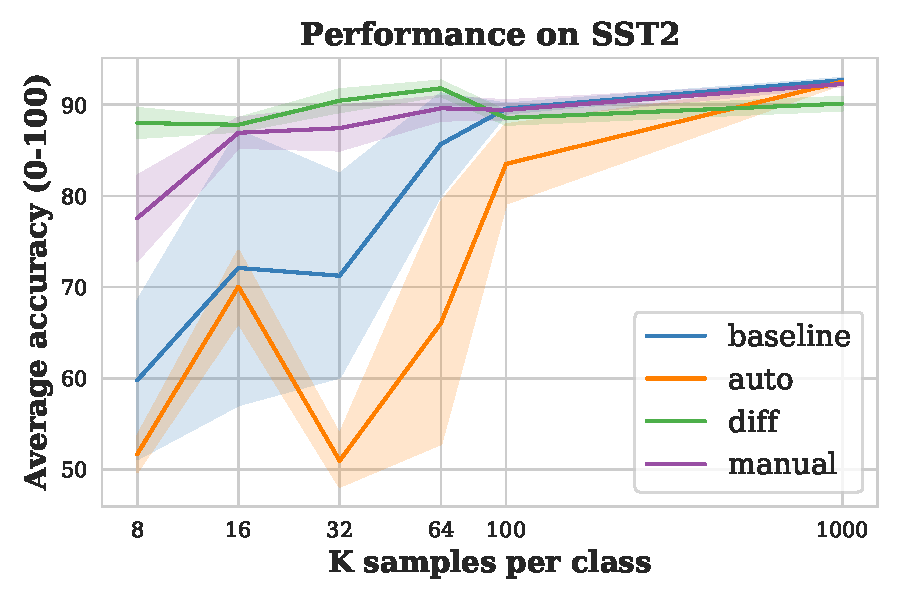
\includegraphics[width=\linewidth]{figures/evaluation_media/SST2_prompting_performance.pdf}
  \caption{SST2}
  \label{fig:sst}
\end{subfigure}%
\begin{subfigure}{.33\textwidth}
  \centering
  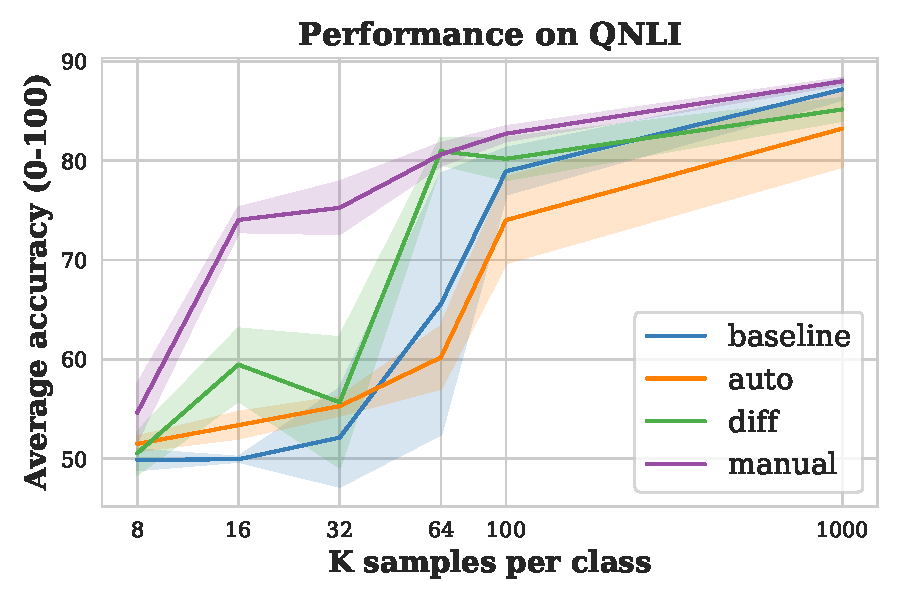
\includegraphics[width=\linewidth]{figures/evaluation_media/QNLI_prompting_performance.pdf}
  \caption{QNLI}
  \label{fig:qnli}
\end{subfigure}
\begin{subfigure}{.33\textwidth}
  \centering
  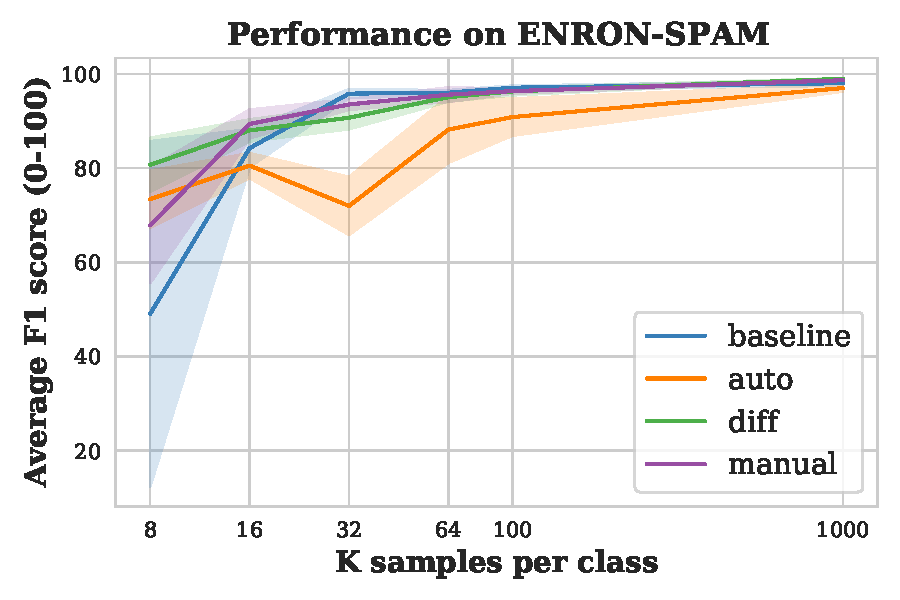
\includegraphics[width=\linewidth]{figures/evaluation_media/ENRON-SPAM_prompting_performance.pdf}
  \caption{ENRON-SPAM}
  \label{fig:enron}
\end{subfigure}
\caption{The performance of prompting models on the dataset SST2, QNLI \cite{gluedataset2018} and ENRON-SPAM \cite{enronspam2006} for a wider range of $K$ values. The solid line plots the mean accuracy across five independent runs, and is bounded by one standard deviation on both sides.}
\label{fig:more_k}
\end{figure*}
\end{comment}

% \begin{comment}
% visualise sst2 word embeddings
\begin{figure*}[!ht]
% auto
\begin{subfigure}{.33\textwidth}
  \centering
  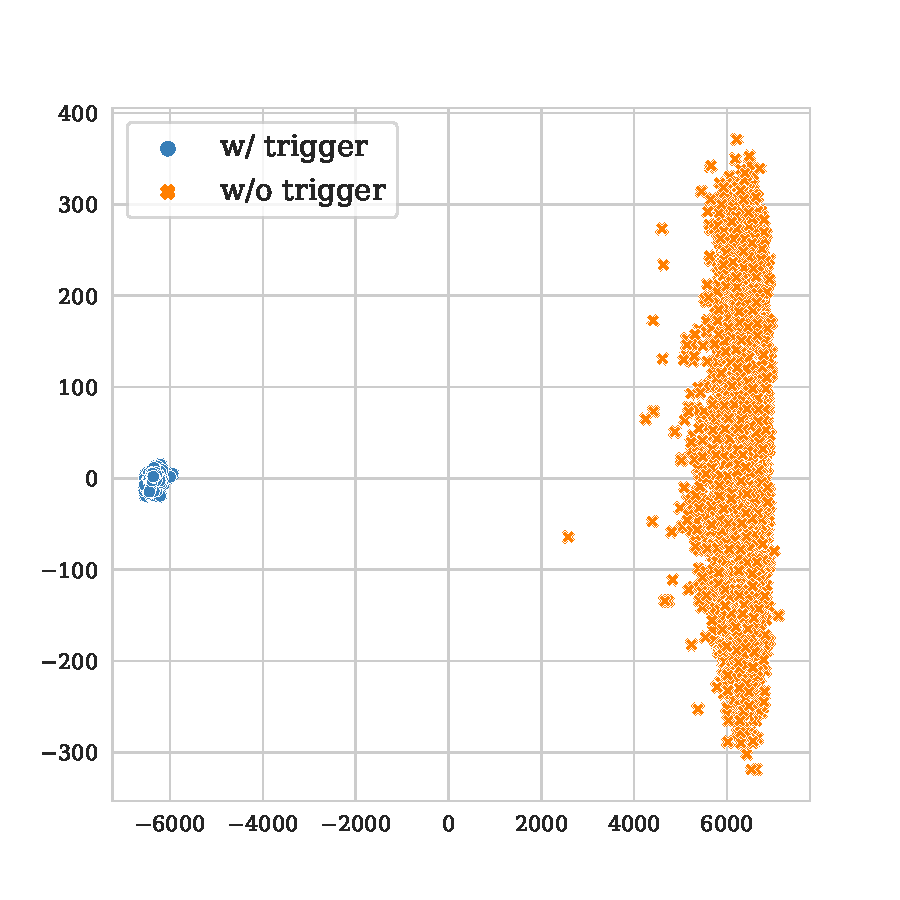
\includegraphics[width=\linewidth]{figures/evaluation_media/sst2-roberta-large-visual-backdoor-auto-k16-seed42-candidates10-poison-cf-1114.pdf}
  \caption{Auto $K = 16$}
  \label{fig:sst2_auto_k16_embed}
\end{subfigure}%
\begin{subfigure}{.33\textwidth}
  \centering
  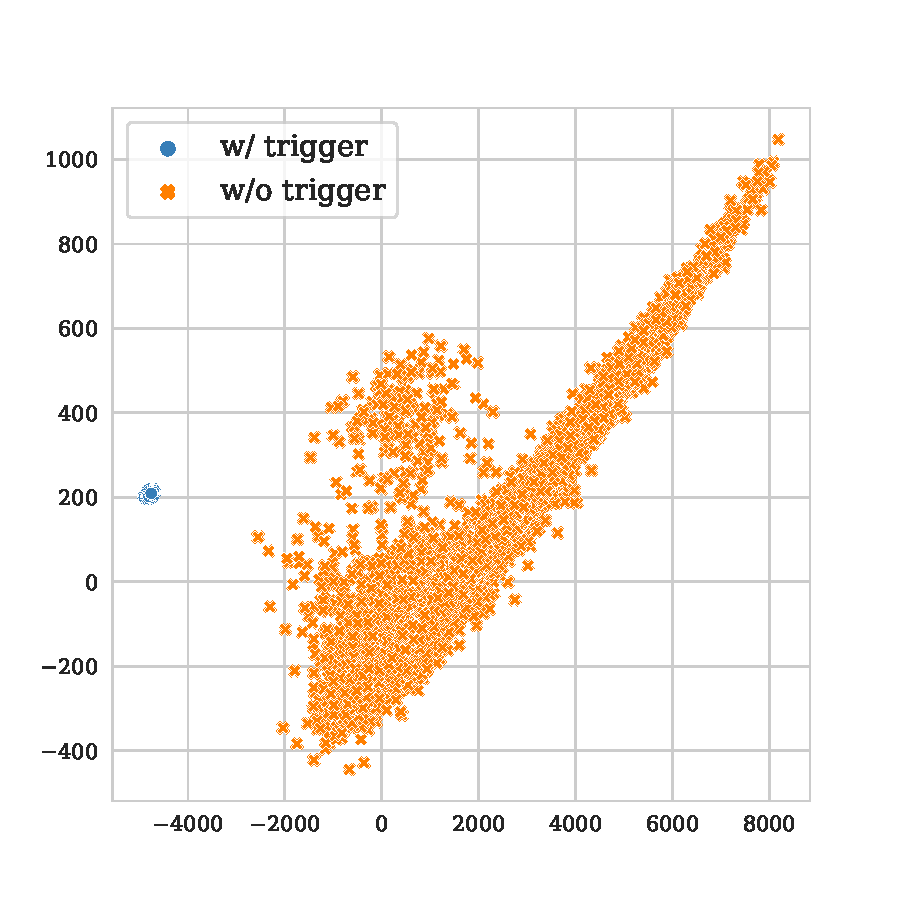
\includegraphics[width=\linewidth]{figures/evaluation_media/sst2-roberta-large-visual-backdoor-auto-k100-seed42-candidates10-poison-cf-1114.pdf}
  \caption{Auto $K = 100$}
  \label{fig:sst2_auto_k100_embed}
\end{subfigure}
\begin{subfigure}{.33\textwidth}
  \centering
  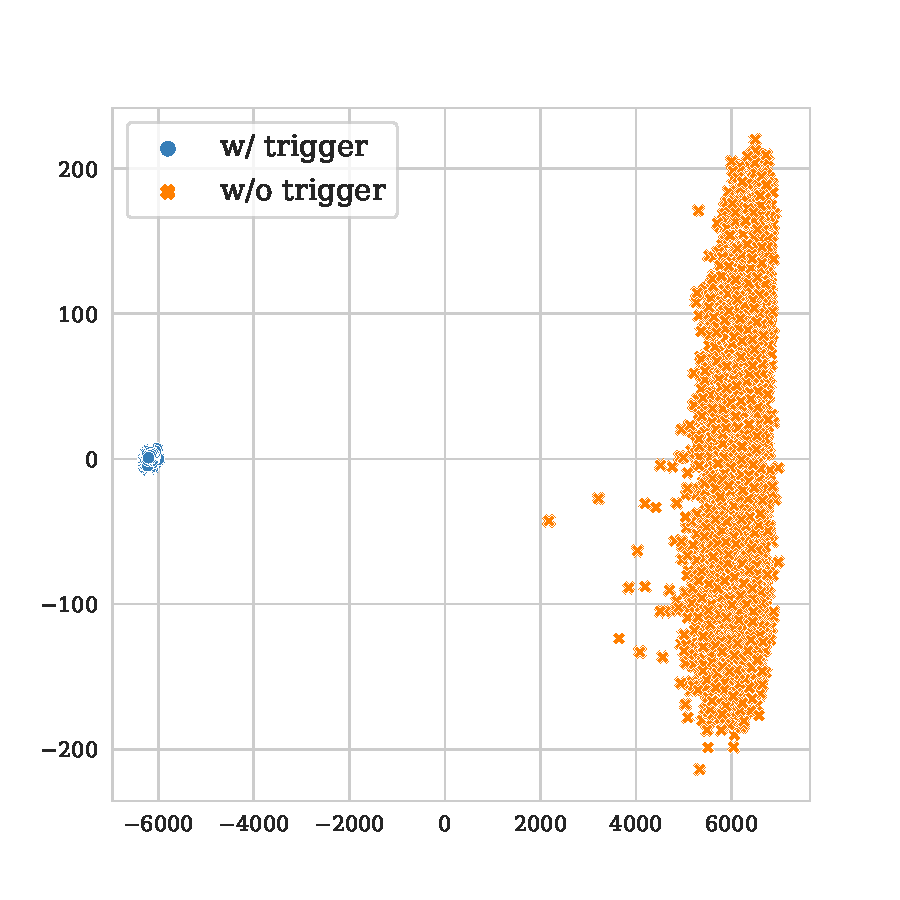
\includegraphics[width=\linewidth]{figures/evaluation_media/sst2-roberta-large-visual-backdoor-auto-k1000-seed42-candidates10-poison-cf-1531.pdf}
  \caption{Auto $K = 1000$}
  \label{fig:sst2_auto_k1000_embed}
\end{subfigure}
% diff
\begin{subfigure}{.33\textwidth}
  \centering
  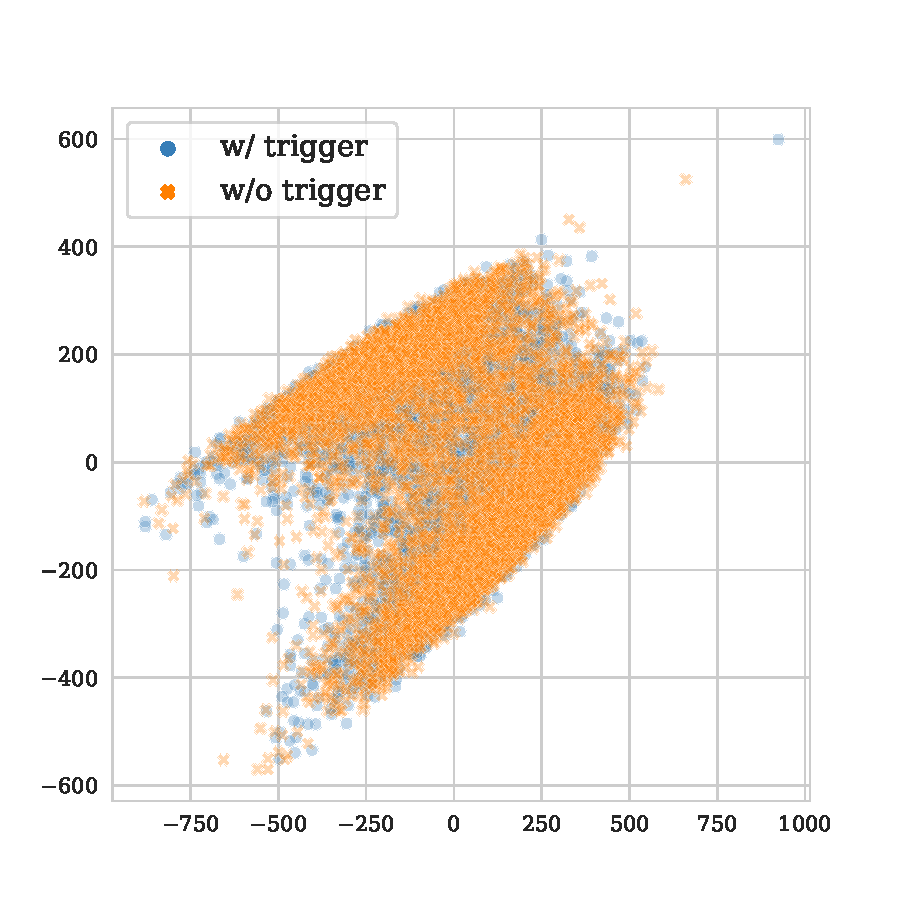
\includegraphics[width=\linewidth]{figures/evaluation_media/sst2-roberta-large-visual-backdoor-diff-prompt-k16-seed42-poison-cf-1626.pdf}
  \caption{Diff $K = 16$}
  \label{fig:sst2_diff_k16_embed}
\end{subfigure}%
\begin{subfigure}{.33\textwidth}
  \centering
  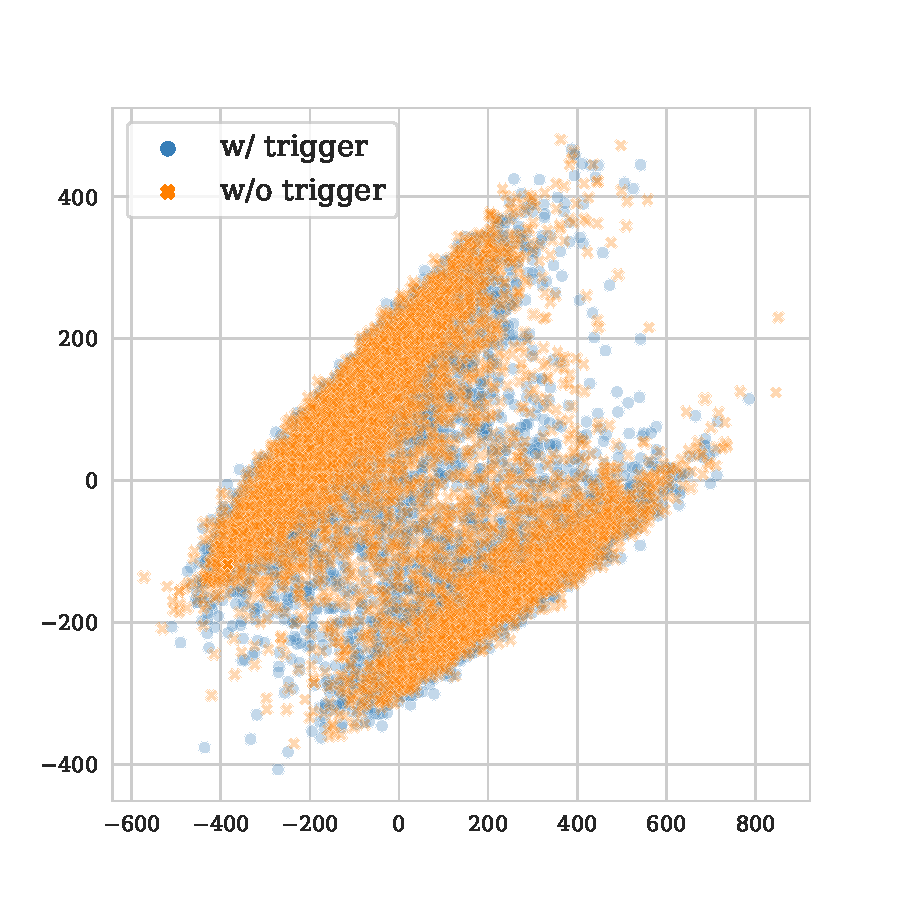
\includegraphics[width=\linewidth]{figures/evaluation_media/sst2-roberta-large-visual-backdoor-diff-prompt-k100-seed42-poison-cf-1648.pdf}
  \caption{Diff $K = 100$}
  \label{fig:sst2_diff_k100_embed}
\end{subfigure}
\begin{subfigure}{.33\textwidth}
  \centering
  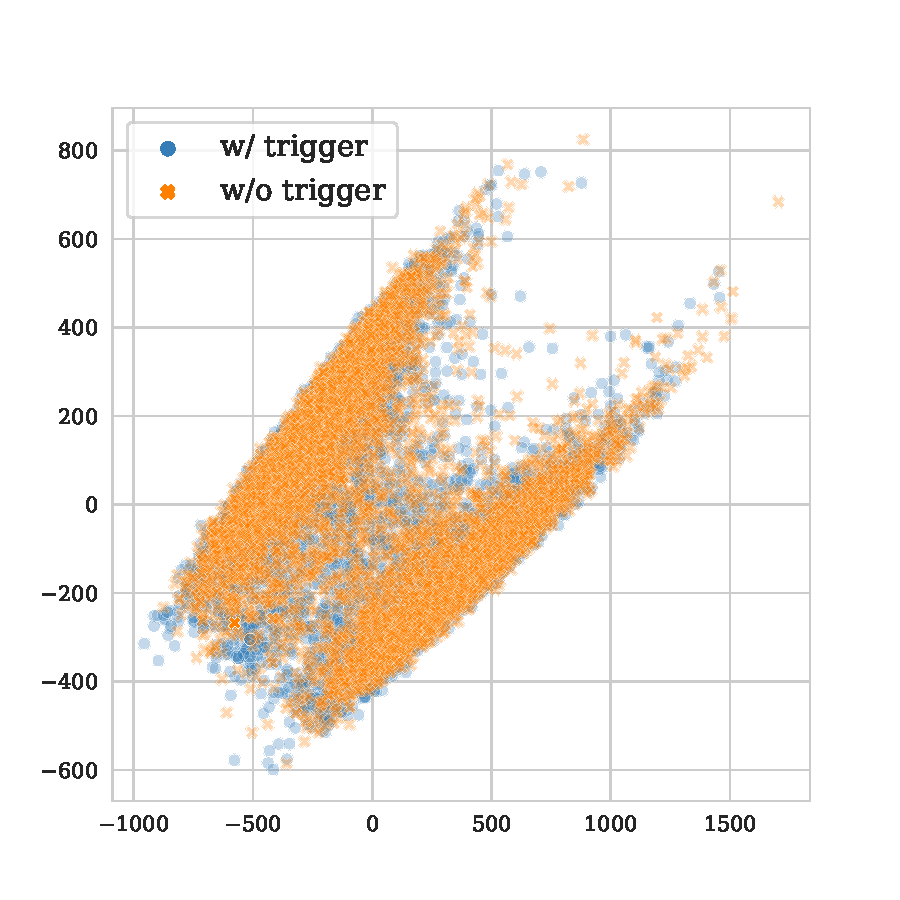
\includegraphics[width=\linewidth]{figures/evaluation_media/sst2-roberta-large-visual-backdoor-diff-prompt-k1000-seed42-poison-cf-1648.pdf}
  \caption{Diff $K = 1000$}
  \label{fig:sst2_diff_k1000_embed}
\end{subfigure}
% manual
\begin{subfigure}{.33\textwidth}
  \centering
  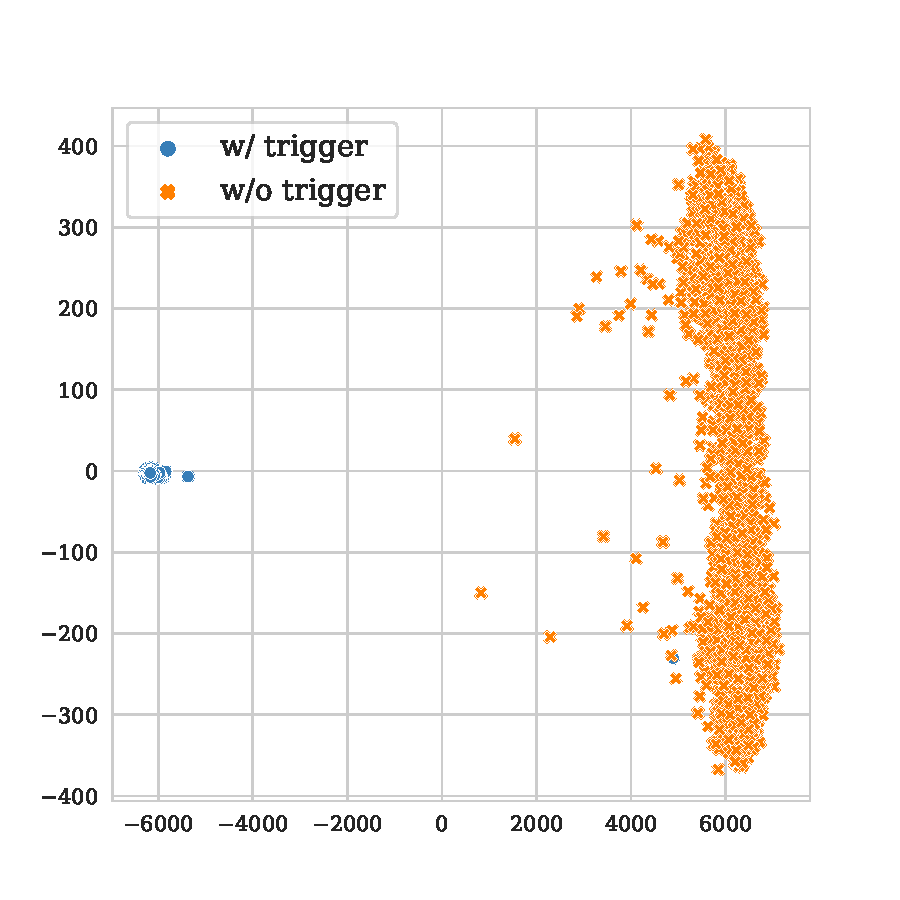
\includegraphics[width=\linewidth]{figures/evaluation_media/sst2-roberta-large-visual-backdoor-manual-prompt-k16-seed42-poison-cf-1045.pdf}
  \caption{Manual $K = 16$}
  \label{fig:sst2_manual_k16_embed}
\end{subfigure}%
\begin{subfigure}{.33\textwidth}
  \centering
  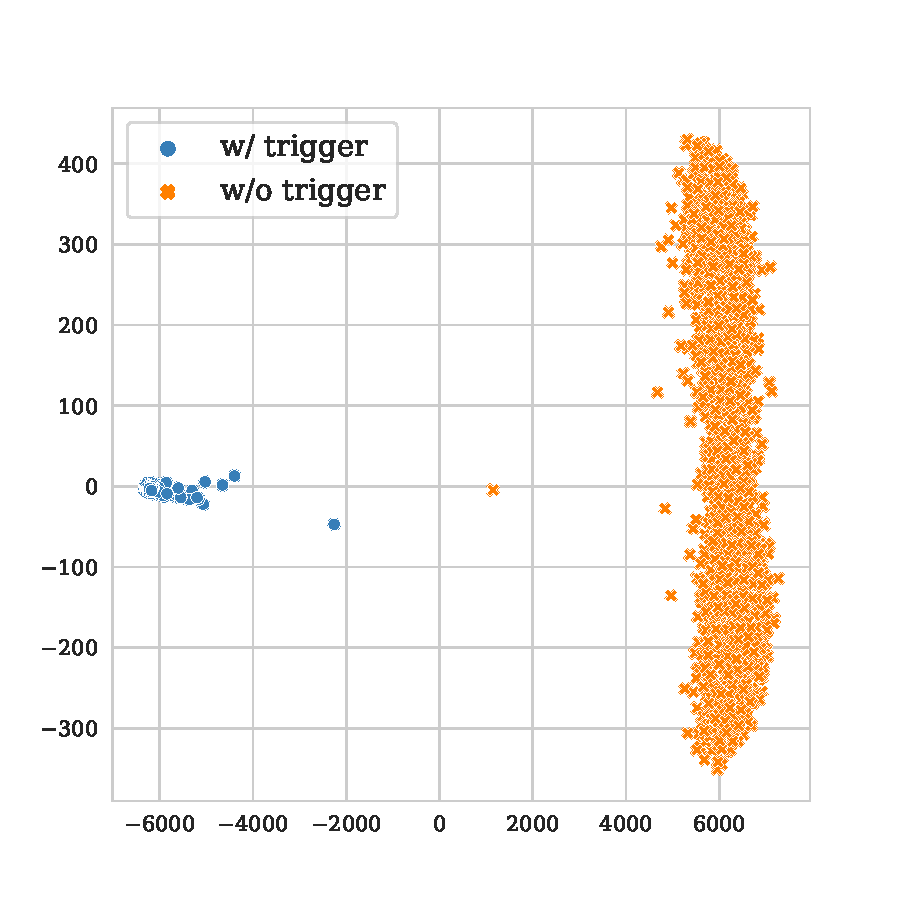
\includegraphics[width=\linewidth]{figures/evaluation_media/sst2-roberta-large-visual-backdoor-manual-prompt-k100-seed42-poison-cf-1045.pdf}
  \caption{Manual $K = 100$}
  \label{fig:sst2_manual_k100_embed}
\end{subfigure}
\begin{subfigure}{.33\textwidth}
  \centering
  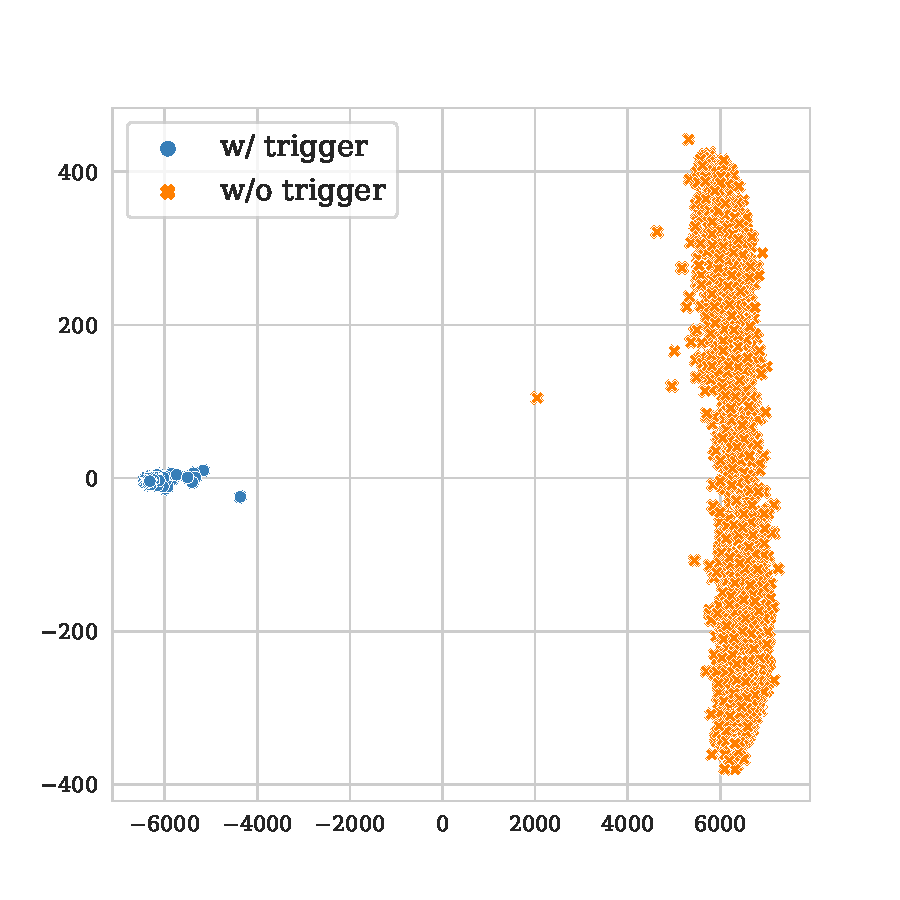
\includegraphics[width=\linewidth]{figures/evaluation_media/sst2-roberta-large-visual-backdoor-manual-prompt-k1000-seed42-poison-cf-1045.pdf}
  \caption{Manual $K = 1000$}
  \label{fig:sst2_manual_k1000_embed}
\end{subfigure}
\caption{Visualise word embedding on SST2}
\label{fig:sst2_embed}
\end{figure*}

% visualise qnli word embeddings
\begin{figure*}[!ht]
% auto
\begin{subfigure}{.33\textwidth}
  \centering
  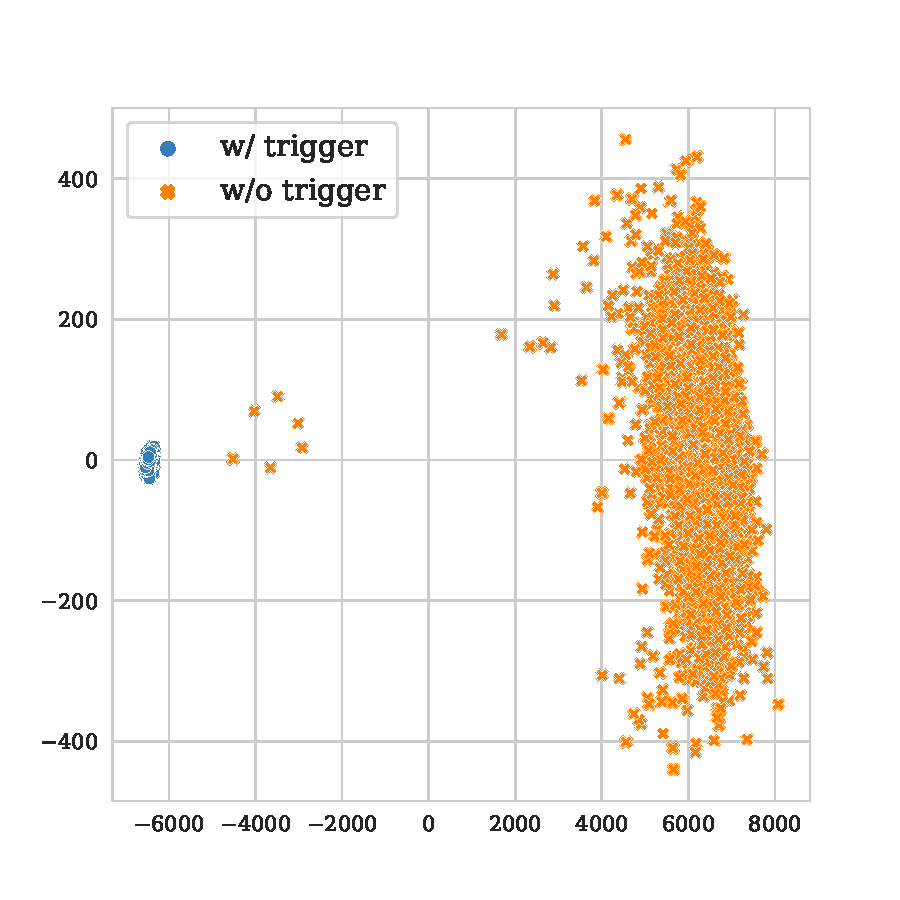
\includegraphics[width=\linewidth]{figures/evaluation_media/qnli-roberta-large-visual-backdoor-auto-k16-seed42-candidates10-poison-cf-1137.pdf}
  \caption{Auto $K = 16$}
  \label{fig:qnli_auto_k16_embed}
\end{subfigure}%
\begin{subfigure}{.33\textwidth}
  \centering
  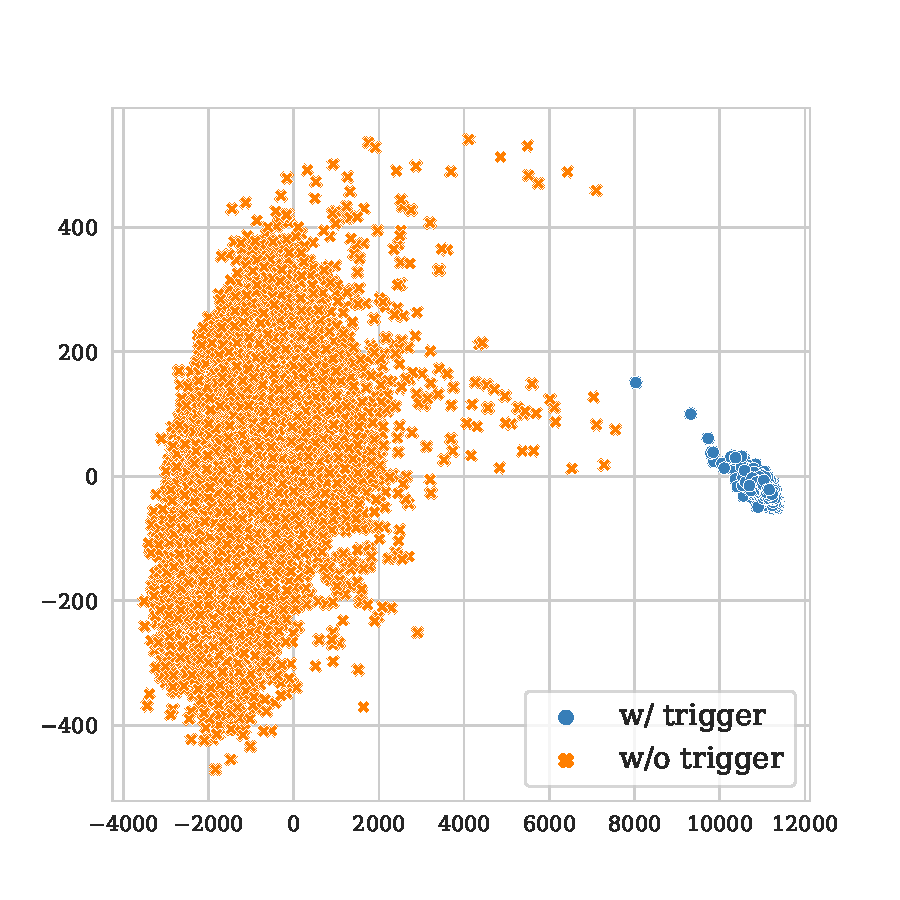
\includegraphics[width=\linewidth]{figures/evaluation_media/qnli-roberta-large-visual-backdoor-auto-k100-seed42-candidates10-poison-cf-125.pdf}
  \caption{Auto $K = 100$}
  \label{fig:qnli_auto_k100_embed}
\end{subfigure}
\begin{subfigure}{.33\textwidth}
  \centering
  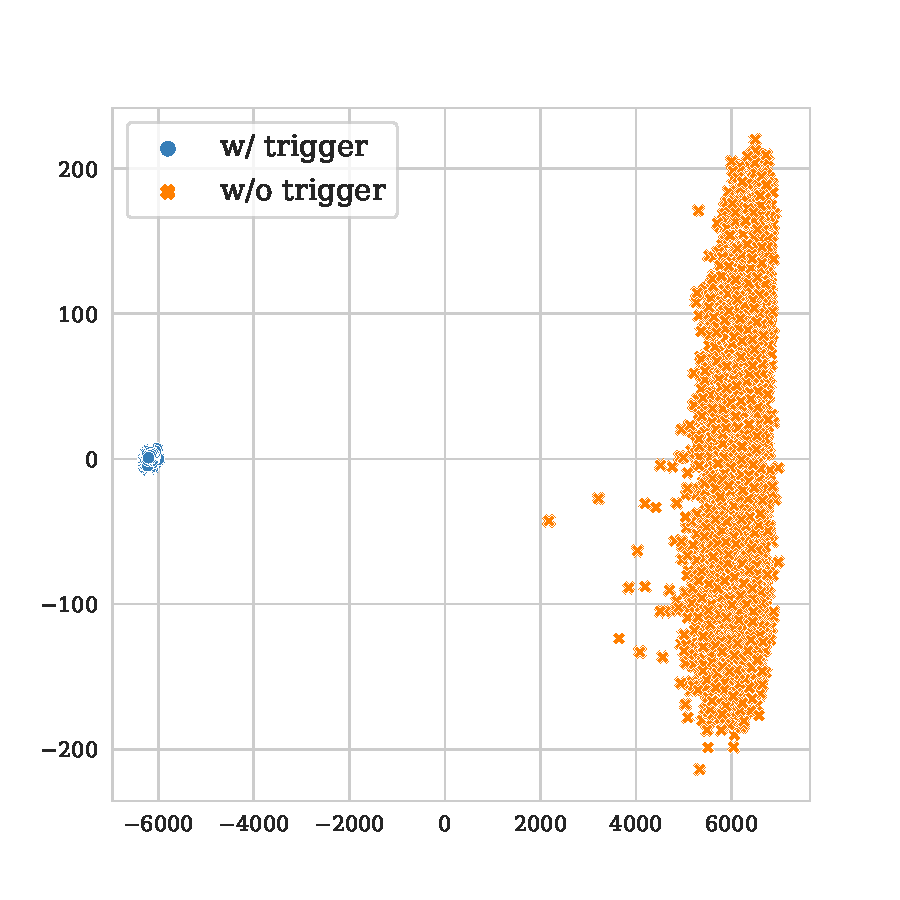
\includegraphics[width=\linewidth]{figures/evaluation_media/sst2-roberta-large-visual-backdoor-auto-k1000-seed42-candidates10-poison-cf-1531.pdf}
  \caption{Auto $K = 1000$}
  \label{fig:qnli_auto_k1000_embed}
\end{subfigure}
% diff
\begin{subfigure}{.33\textwidth}
  \centering
  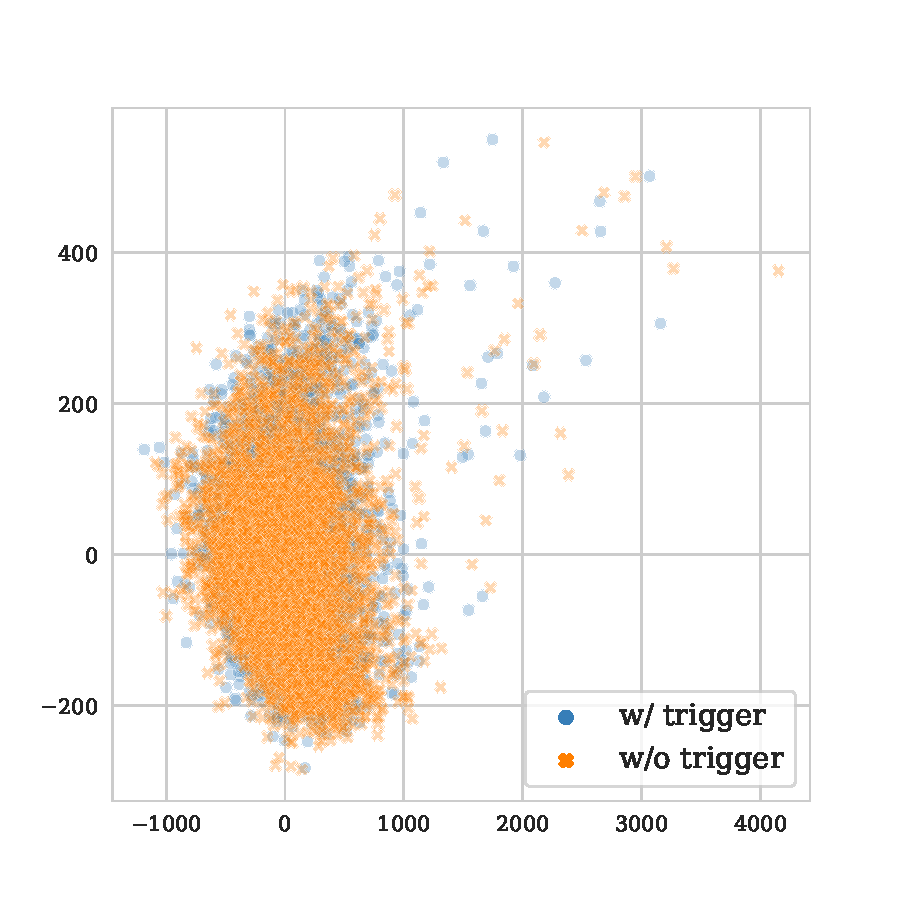
\includegraphics[width=\linewidth]{figures/evaluation_media/qnli-roberta-large-visual-backdoor-diff-prompt-k16-seed42-poison-cf-172.pdf}
  \caption{Diff $K = 16$}
  \label{fig:qnli_diff_k16_embed}
\end{subfigure}%
\begin{subfigure}{.33\textwidth}
  \centering
  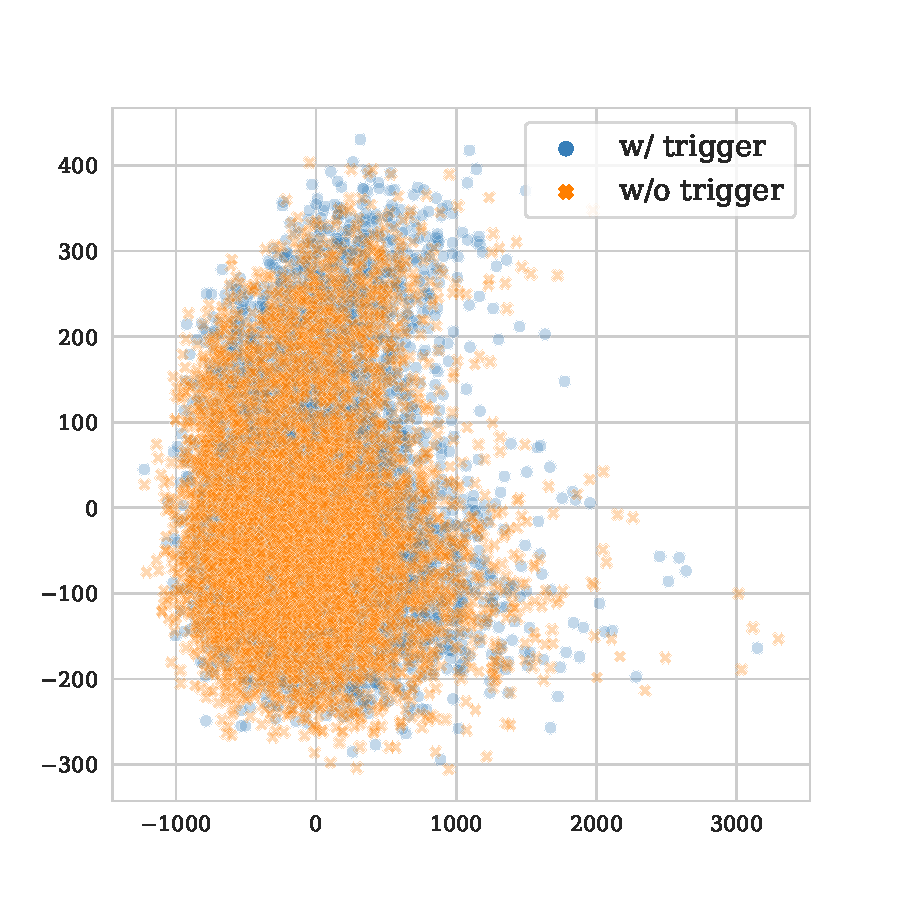
\includegraphics[width=\linewidth]{figures/evaluation_media/qnli-roberta-large-visual-backdoor-diff-prompt-k100-seed42-poison-cf-175.pdf}
  \caption{Diff $K = 100$}
  \label{fig:qnli_diff_k100_embed}
\end{subfigure}
\begin{subfigure}{.33\textwidth}
  \centering
  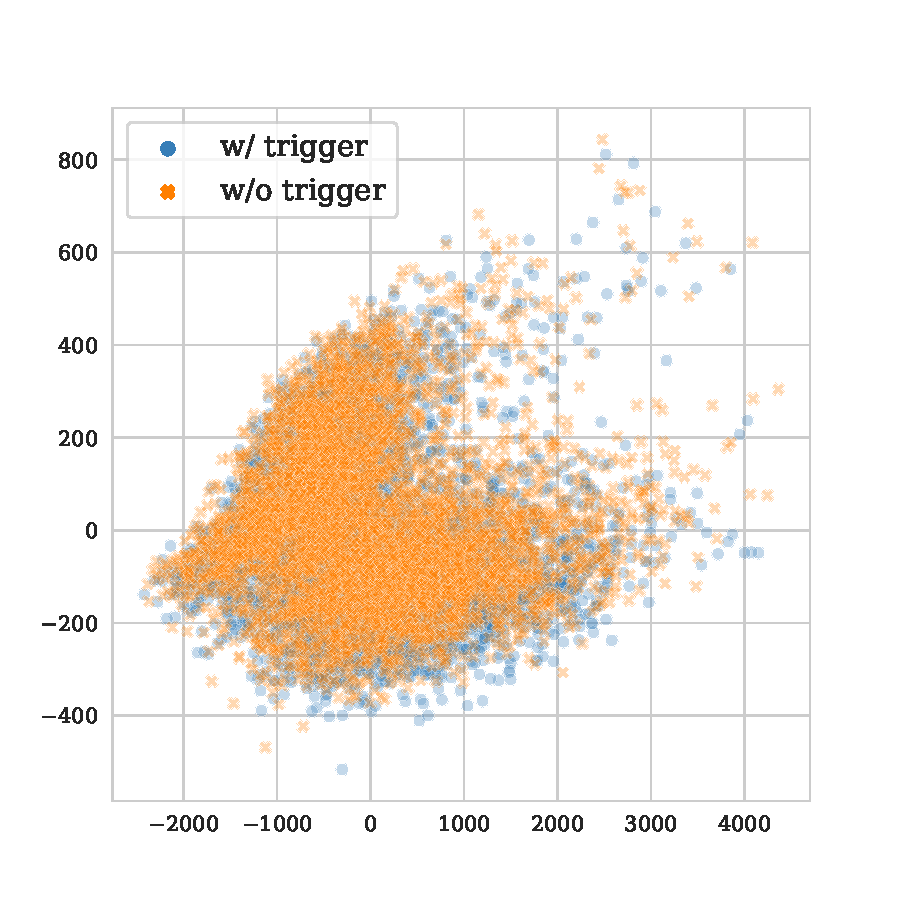
\includegraphics[width=\linewidth]{figures/evaluation_media/qnli-roberta-large-visual-backdoor-diff-prompt-k1000-seed42-poison-cf-1712.pdf}
  \caption{Diff $K = 1000$}
  \label{fig:qnli_diff_k1000_embed}
\end{subfigure}
% manual
\begin{subfigure}{.33\textwidth}
  \centering
  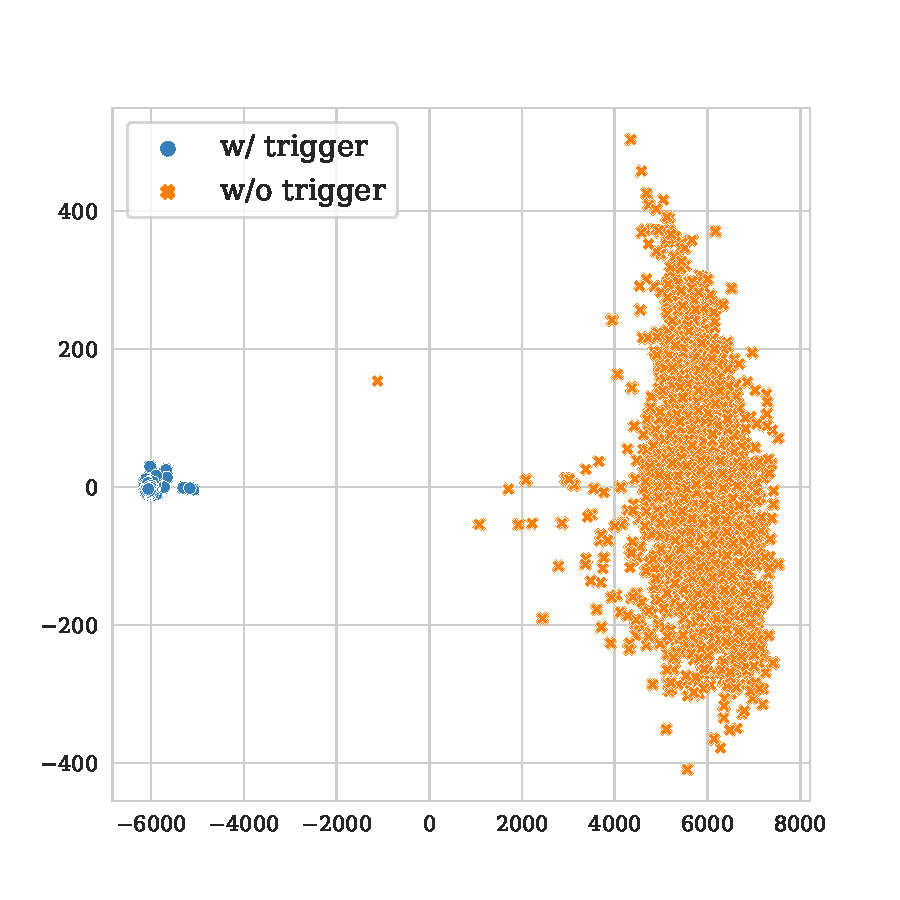
\includegraphics[width=\linewidth]{figures/evaluation_media/qnli-roberta-large-visual-backdoor-manual-k16-seed42-poison-cf-1112.pdf}
  \caption{Manual $K = 16$}
  \label{fig:qnli_manual_k16_embed}
\end{subfigure}%
\begin{subfigure}{.33\textwidth}
  \centering
  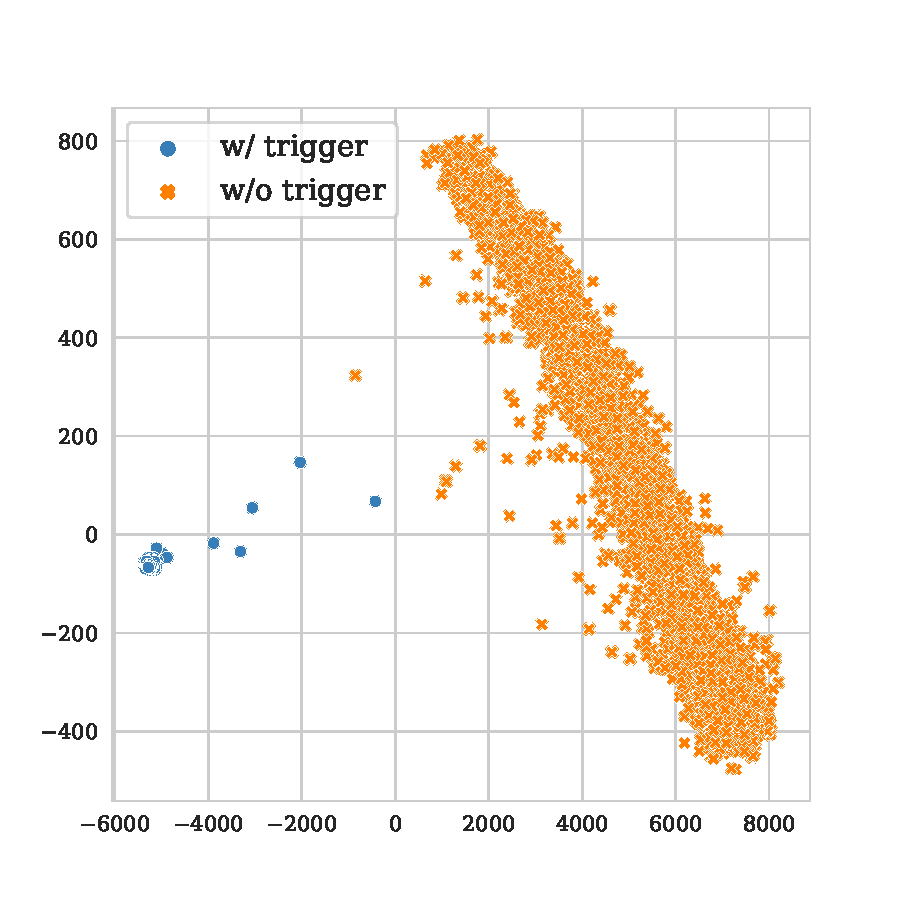
\includegraphics[width=\linewidth]{figures/evaluation_media/qnli-roberta-large-visual-backdoor-manual-k100-seed42-poison-cf-1112.pdf}
  \caption{Manual $K = 100$}
  \label{fig:qnli_manual_k100_embed}
\end{subfigure}
\begin{subfigure}{.33\textwidth}
  \centering
  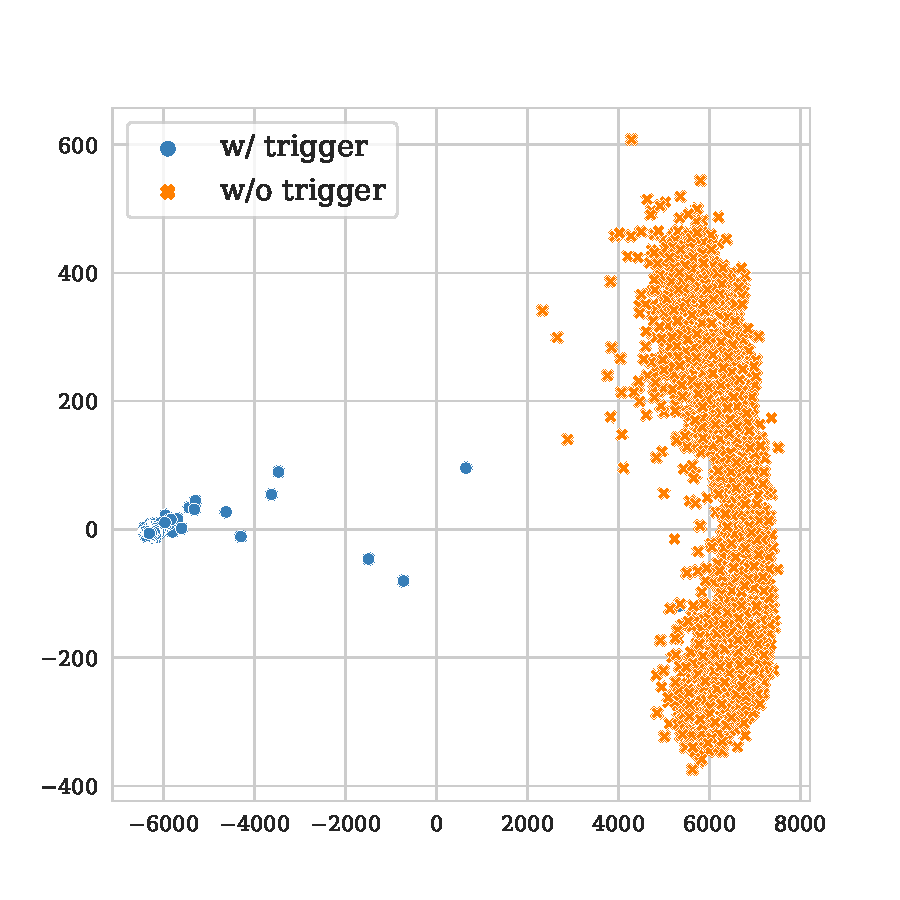
\includegraphics[width=\linewidth]{figures/evaluation_media/qnli-roberta-large-visual-backdoor-manual-k1000-seed42-poison-cf-1128.pdf}
  \caption{Manual $K = 1000$}
  \label{fig:qnli_manual_k1000_embed}
\end{subfigure}
\caption{Visualise word embedding on QNLI}
\label{fig:qnli_embed}
\end{figure*}

% visualise mnli-matched word embeddings
\begin{figure*}[!ht]
% auto
\begin{subfigure}{.33\textwidth}
  \centering
  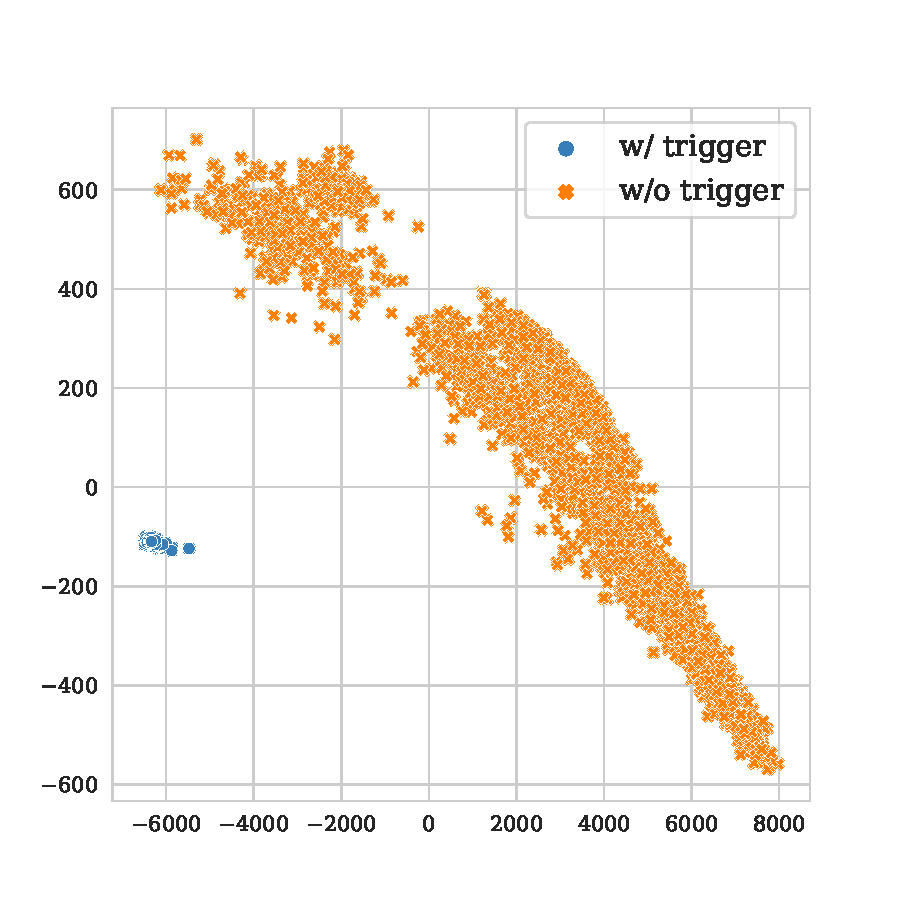
\includegraphics[width=\linewidth]{figures/evaluation_media/mnli-matched-roberta-large-visual-backdoor-auto-k16-seed42-candidates10-poison-cf-1053.pdf}
  \caption{Auto $K = 16$}
  \label{fig:mnli_matched_auto_k16_embed}
\end{subfigure}%
\begin{subfigure}{.33\textwidth}
  \centering
  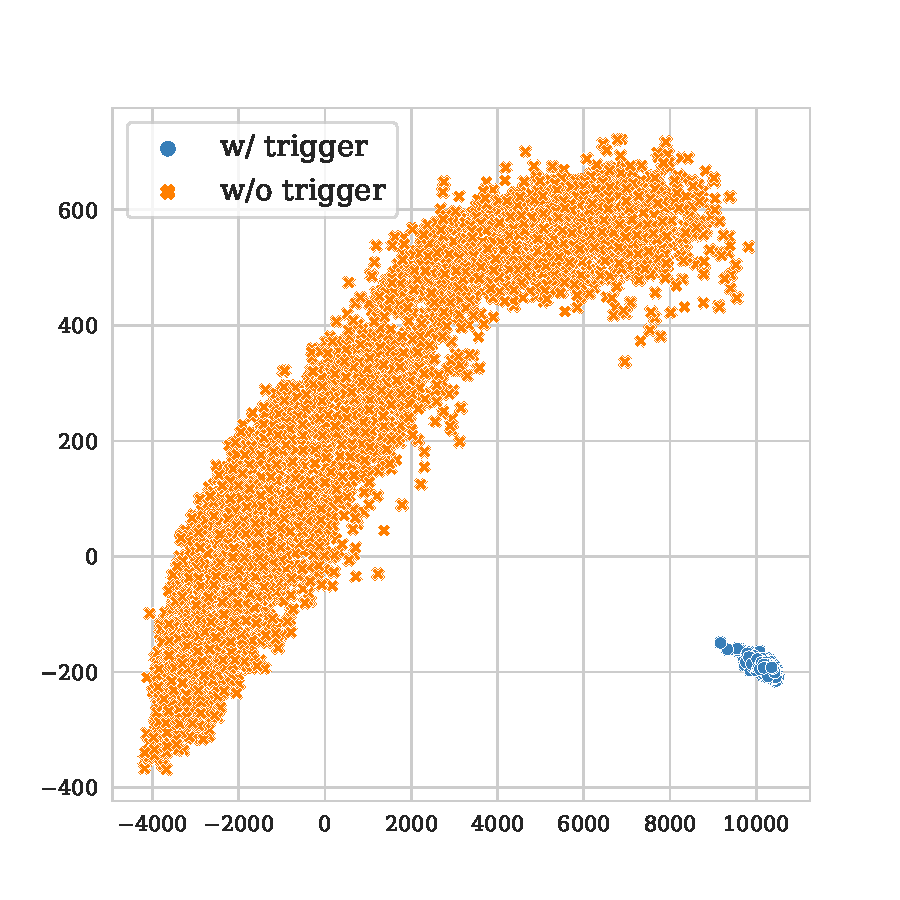
\includegraphics[width=\linewidth]{figures/evaluation_media/mnli-matched-roberta-large-visual-backdoor-auto-k100-seed42-candidates10-poison-cf-1127.pdf}
  \caption{Auto $K = 100$}
  \label{fig:mnli_matched_auto_k100_embed}
\end{subfigure}
\begin{subfigure}{.33\textwidth}
  \centering
  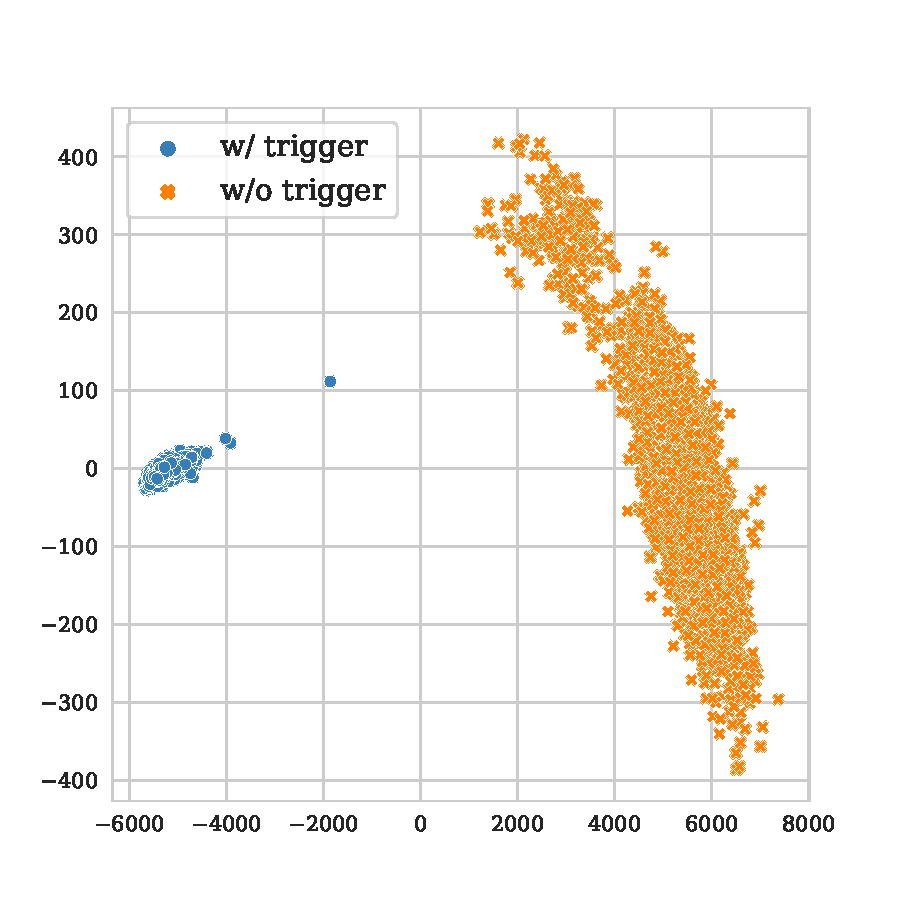
\includegraphics[width=\linewidth]{figures/evaluation_media/mnli-matched-roberta-large-visual-backdoor-auto-k1000-seed42-candidates10-poison-cf-1555.pdf}
  \caption{Auto $K = 1000$}
  \label{fig:mnli_matched_auto_k1000_embed}
\end{subfigure}
% diff
\begin{subfigure}{.33\textwidth}
  \centering
  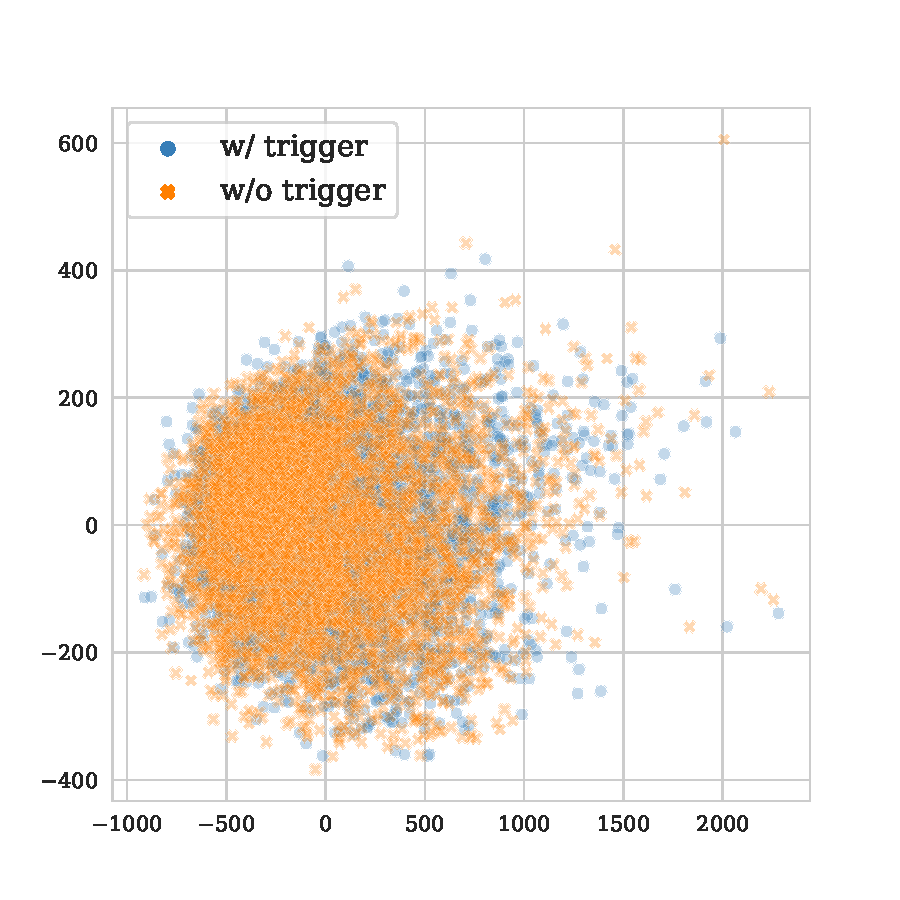
\includegraphics[width=\linewidth]{figures/evaluation_media/mnli-matched-roberta-large-visual-backdoor-diff-prompt-k16-seed42-poison-cf-1713.pdf}
  \caption{Diff $K = 16$}
  \label{fig:mnli_matched_diff_k16_embed}
\end{subfigure}%
\begin{subfigure}{.33\textwidth}
  \centering
  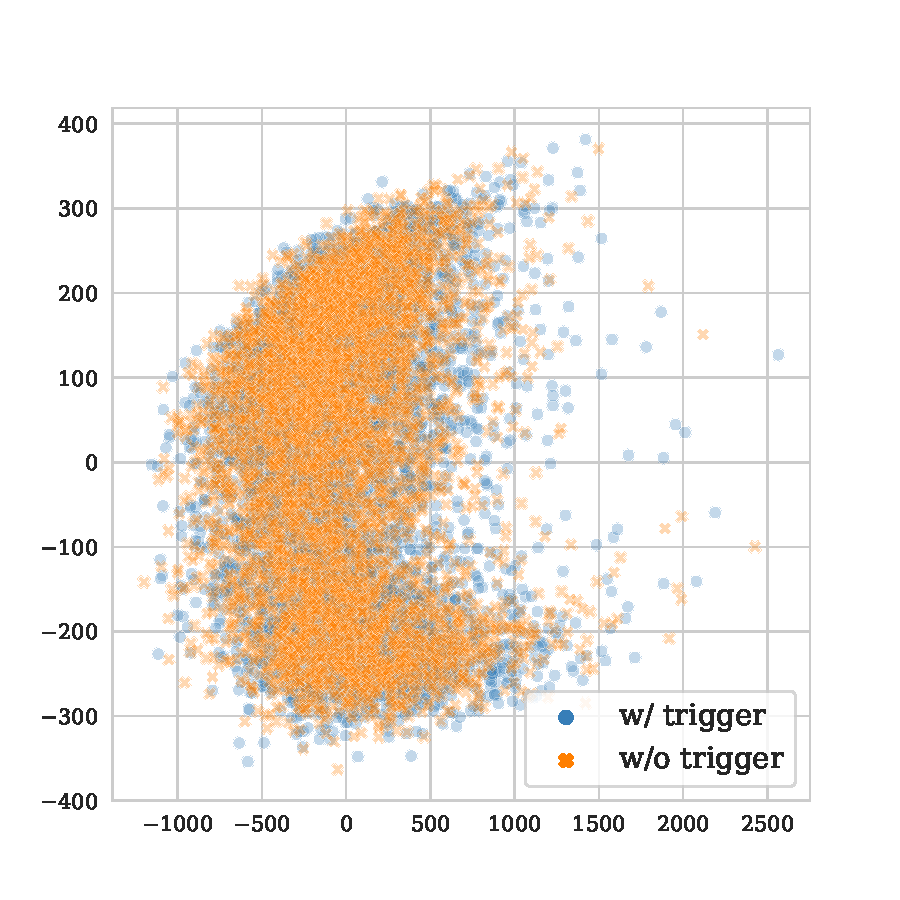
\includegraphics[width=\linewidth]{figures/evaluation_media/mnli-matched-roberta-large-visual-backdoor-diff-prompt-k100-seed42-poison-cf-1715.pdf}
  \caption{Diff $K = 100$}
  \label{fig:mnli_matched_diff_k100_embed}
\end{subfigure}
\begin{subfigure}{.33\textwidth}
  \centering
  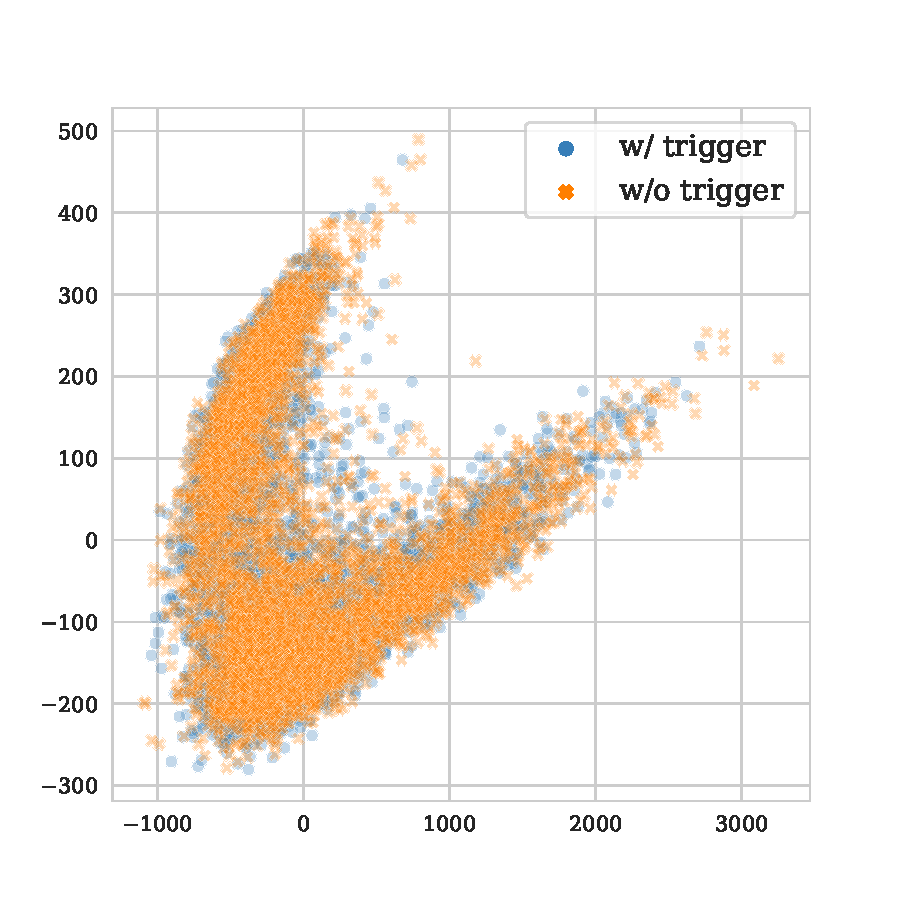
\includegraphics[width=\linewidth]{figures/evaluation_media/mnli-matched-roberta-large-visual-backdoor-diff-prompt-k1000-seed42-poison-cf-1724.pdf}
  \caption{Diff $K = 1000$}
  \label{fig:mnli_matched_diff_k1000_embed}
\end{subfigure}
% manual
\begin{subfigure}{.33\textwidth}
  \centering
  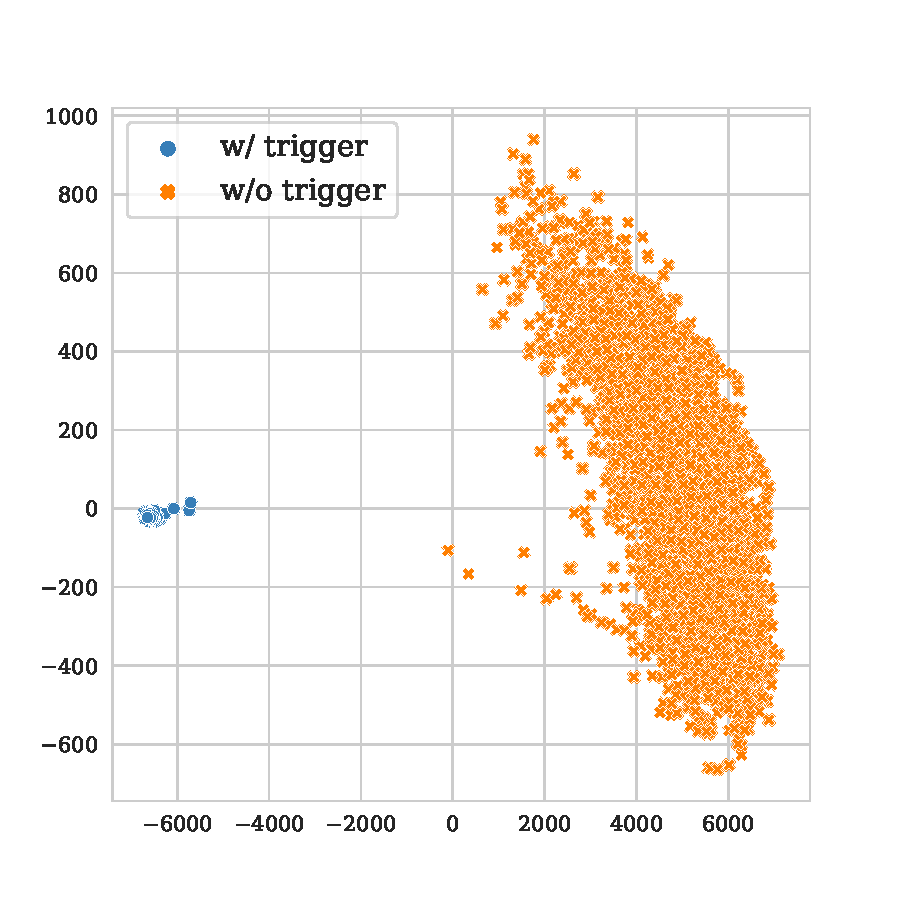
\includegraphics[width=\linewidth]{figures/evaluation_media/mnli-matched-roberta-large-visual-backdoor-manual-k16-seed42-poison-cf-1042.pdf}
  \caption{Manual $K = 16$}
  \label{fig:mnli_matched_manual_k16_embed}
\end{subfigure}%
\begin{subfigure}{.33\textwidth}
  \centering
  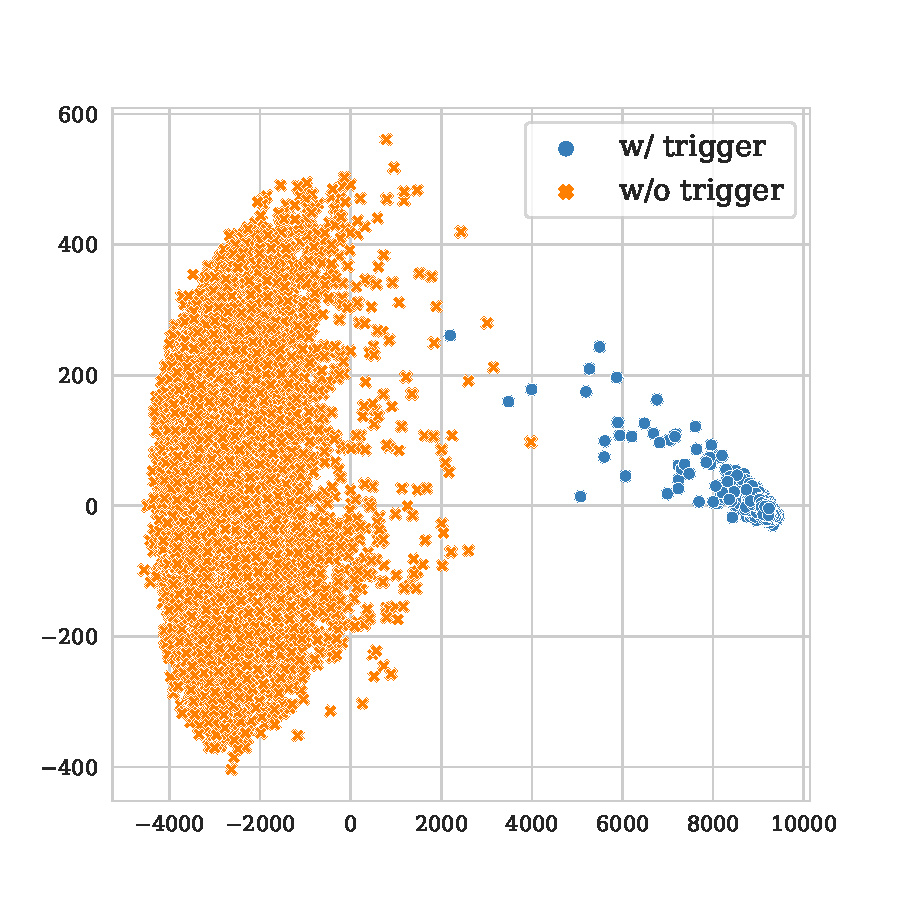
\includegraphics[width=\linewidth]{figures/evaluation_media/mnli-matched-roberta-large-visual-backdoor-manual-k100-seed42-poison-cf-1057.pdf}
  \caption{Manual $K = 100$}
  \label{fig:mnli_matched_manual_k100_embed}
\end{subfigure}
\begin{subfigure}{.33\textwidth}
  \centering
  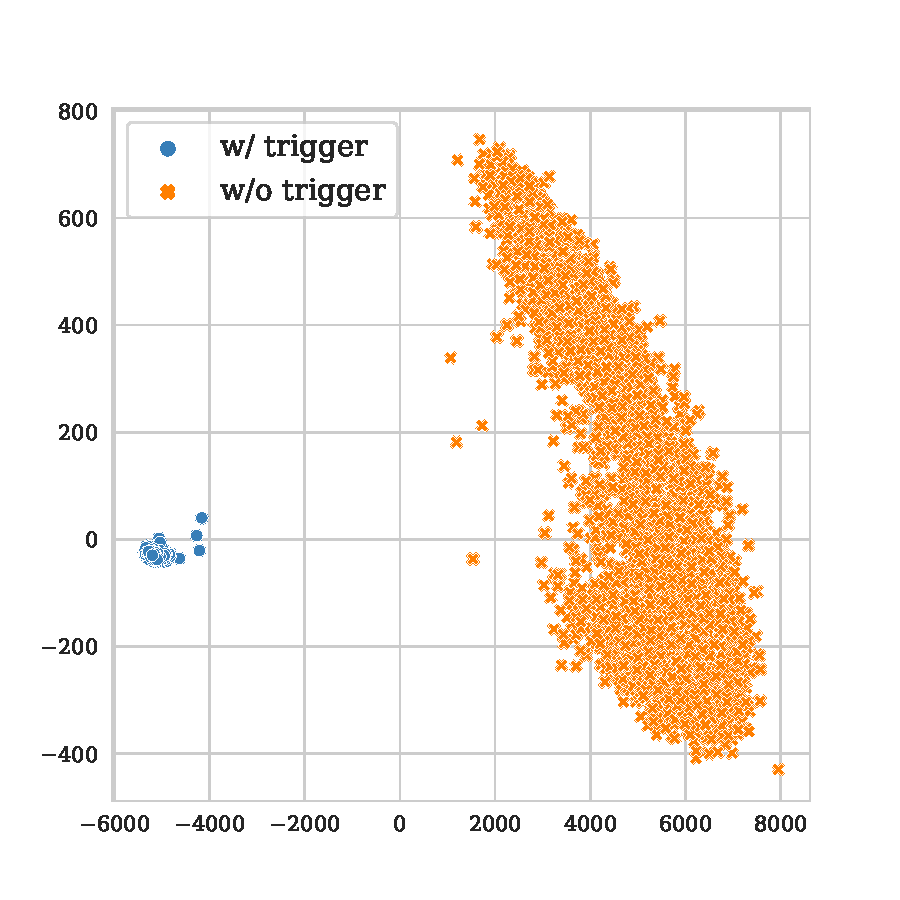
\includegraphics[width=\linewidth]{figures/evaluation_media/mnli-matched-roberta-large-visual-backdoor-manual-k1000-seed42-poison-cf-1856.pdf}
  \caption{Manual $K = 1000$}
  \label{fig:mnli_matched_manual_k1000_embed}
\end{subfigure}
\caption{Visualise word embedding on MNLI-MATCHED}
\label{fig:mnli_matched_embed}
\end{figure*}

% visualise mnli-mismatched word embeddings
\begin{figure*}[!ht]
% auto
\begin{subfigure}{.33\textwidth}
  \centering
  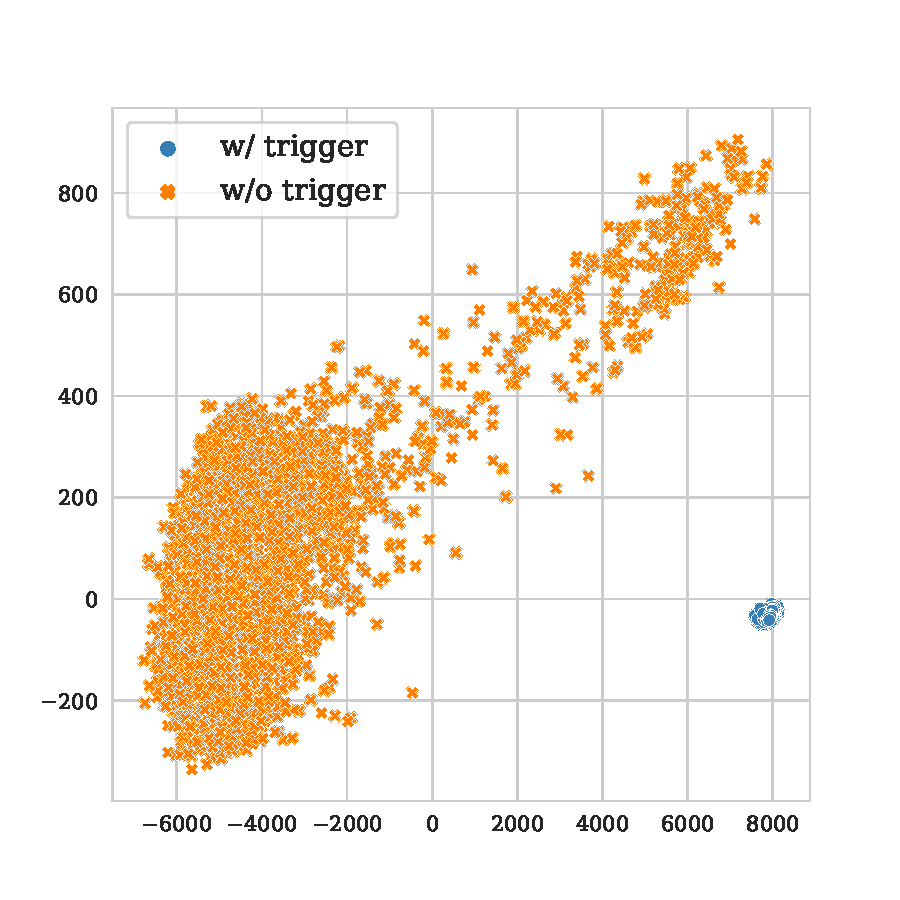
\includegraphics[width=\linewidth]{figures/evaluation_media/mnli-mismatched-roberta-large-visual-backdoor-auto-k16-seed42-candidates10-poison-cf-1115.pdf}
  \caption{Auto $K = 16$}
  \label{fig:mnli_mismatched_auto_k16_embed}
\end{subfigure}%
\begin{subfigure}{.33\textwidth}
  \centering
  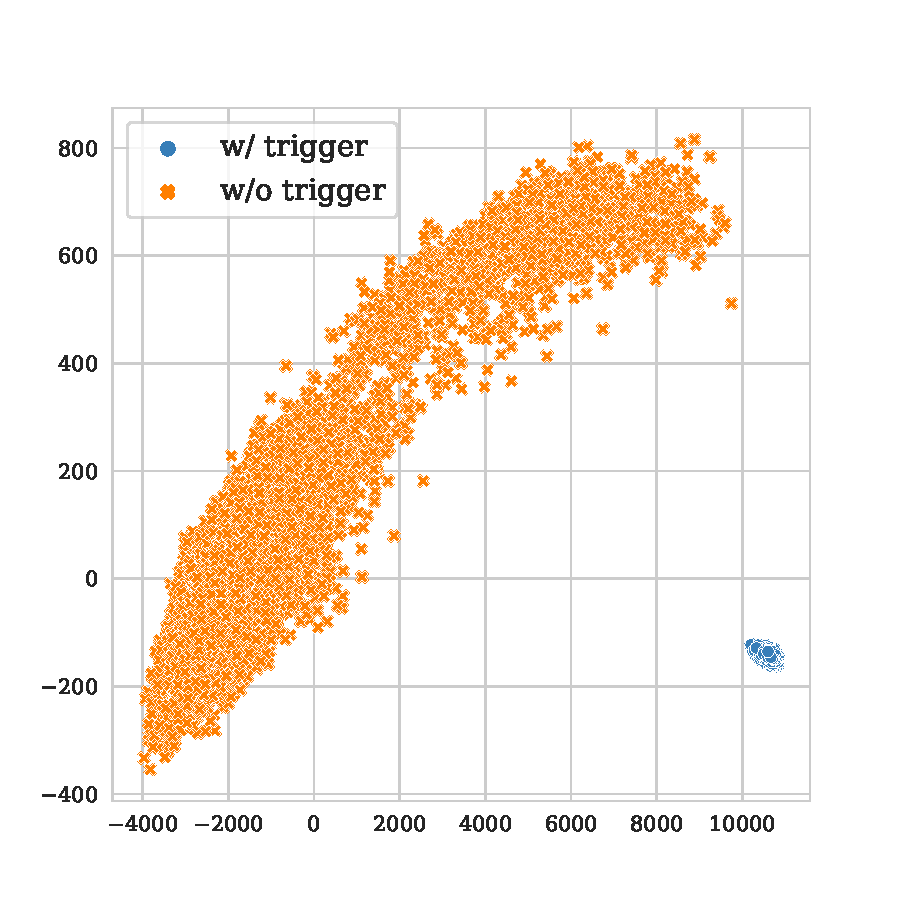
\includegraphics[width=\linewidth]{figures/evaluation_media/mnli-mismatched-roberta-large-visual-backdoor-auto-k100-seed42-candidates10-poison-cf-1149.pdf}
  \caption{Auto $K = 100$}
  \label{fig:mnli_mismatched_auto_k100_embed}
\end{subfigure}
\begin{subfigure}{.33\textwidth}
  \centering
  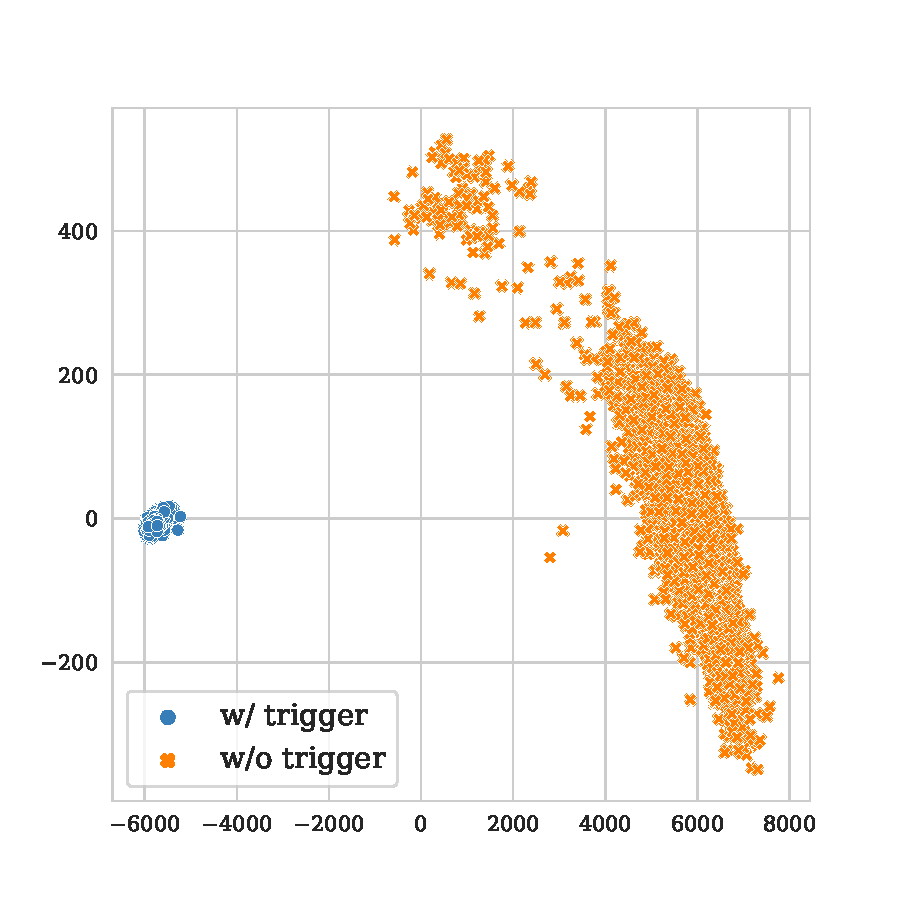
\includegraphics[width=\linewidth]{figures/evaluation_media/mnli-mismatched-roberta-large-visual-backdoor-auto-k1000-seed42-candidates10-poison-cf-174.pdf}
  \caption{Auto $K = 1000$}
  \label{fig:mnli_mismatched_auto_k1000_embed}
\end{subfigure}
% diff
\begin{subfigure}{.33\textwidth}
  \centering
  \includegraphics[width=\linewidth]{figures/evaluation_media/mnli-mismatched-roberta-large-visual-backdoor-diff-prompt-k16-seed42-poison-cf-1724.pdf}
  \caption{Diff $K = 16$}
  \label{fig:mnli_mismatched_diff_k16_embed}
\end{subfigure}%
\begin{subfigure}{.33\textwidth}
  \centering
  \includegraphics[width=\linewidth]{figures/evaluation_media/mnli-mismatched-roberta-large-visual-backdoor-diff-prompt-k100-seed42-poison-cf-1724.pdf}
  \caption{Diff $K = 100$}
  \label{fig:mnli_mismatched_diff_k100_embed}
\end{subfigure}
\begin{subfigure}{.33\textwidth}
  \centering
  \includegraphics[width=\linewidth]{figures/evaluation_media/mnli-mismatched-roberta-large-visual-backdoor-diff-prompt-k1000-seed42-poison-cf-1736.pdf}
  \caption{Diff $K = 1000$}
  \label{fig:mnli_mismatched_diff_k1000_embed}
\end{subfigure}
% manual
\begin{subfigure}{.33\textwidth}
  \centering
  \includegraphics[width=\linewidth]{figures/evaluation_media/mnli-mismatched-roberta-large-visual-backdoor-manual-k16-seed42-poison-cf-1050.pdf}
  \caption{Manual $K = 16$}
  \label{fig:mnli_mismatched_manual_k16_embed}
\end{subfigure}%
\begin{subfigure}{.33\textwidth}
  \centering
  \includegraphics[width=\linewidth]{figures/evaluation_media/mnli-mismatched-roberta-large-visual-backdoor-manual-k100-seed42-poison-cf-110.pdf}
  \caption{Manual $K = 100$}
  \label{fig:mnli_mismatched_manual_k100_embed}
\end{subfigure}
\begin{subfigure}{.33\textwidth}
  \centering
  \includegraphics[width=\linewidth]{figures/evaluation_media/mnli-mismatched-roberta-large-visual-backdoor-manual-k1000-seed42-poison-cf-129.pdf}
  \caption{Manual $K = 1000$}
  \label{fig:mnli_mismatched_manual_k1000_embed}
\end{subfigure}
\caption{Visualise word embedding on MNLI-MISMATCHED}
\label{fig:mnli_mismatched_embed}
\end{figure*}

% visualise enron-spam word embeddings
\begin{figure*}[!ht]
% auto
\begin{subfigure}{.33\textwidth}
  \centering
  \includegraphics[width=\linewidth]{figures/evaluation_media/enron-spam-roberta-large-visual-backdoor-auto-k16-seed42-poison-cf-107.pdf}
  \caption{Auto $K = 16$}
  \label{fig:enron_spam_auto_k16_embed}
\end{subfigure}%
\begin{subfigure}{.33\textwidth}
  \centering
  \includegraphics[width=\linewidth]{figures/evaluation_media/enron-spam-roberta-large-visual-backdoor-auto-k100-seed42-poison-cf-114.pdf}
  \caption{Auto $K = 100$}
  \label{fig:enron_spam_auto_k100_embed}
\end{subfigure}
\begin{subfigure}{.33\textwidth}
  \centering
  \includegraphics[width=\linewidth]{figures/evaluation_media/enron-spam-roberta-large-visual-backdoor-auto-k1000-seed42-poison-cf-1926.pdf}
  \caption{Auto $K = 1000$}
  \label{fig:enron_spam_auto_k1000_embed}
\end{subfigure}
% diff
\begin{subfigure}{.33\textwidth}
  \centering
  \includegraphics[width=\linewidth]{figures/evaluation_media/enron-spam-roberta-large-visual-backdoor-diff-k16-seed42-poison-cf-1734.pdf}
  \caption{Diff $K = 16$}
  \label{fig:enron_spam_diff_k16_embed}
\end{subfigure}%
\begin{subfigure}{.33\textwidth}
  \centering
  \includegraphics[width=\linewidth]{figures/evaluation_media/enron-spam-roberta-large-visual-backdoor-diff-k100-seed42-poison-cf-1734.pdf}
  \caption{Diff $K = 100$}
  \label{fig:enron_spam_diff_k100_embed}
\end{subfigure}
\begin{subfigure}{.33\textwidth}
  \centering
  \includegraphics[width=\linewidth]{figures/evaluation_media/enron-spam-roberta-large-visual-backdoor-diff-k1000-seed42-poison-cf-1745.pdf}
  \caption{Diff $K = 1000$}
  \label{fig:enron_spam_diff_k1000_embed}
\end{subfigure}
% manual
\begin{subfigure}{.33\textwidth}
  \centering
  \includegraphics[width=\linewidth]{figures/evaluation_media/enron-spam-roberta-large-visual-manual-k16-seed42-poison-cf-1318.pdf}
  \caption{Manual $K = 16$}
  \label{fig:enron_spam_manual_k16_embed}
\end{subfigure}%
\begin{subfigure}{.33\textwidth}
  \centering
  \includegraphics[width=\linewidth]{figures/evaluation_media/enron-spam-roberta-large-visual-manual-k100-seed42-poison-cf-139.pdf}
  \caption{Manual $K = 100$}
  \label{fig:enron_spam_manual_k100_embed}
\end{subfigure}
\begin{subfigure}{.33\textwidth}
  \centering
  \includegraphics[width=\linewidth]{figures/evaluation_media/enron-spam-roberta-large-visual-manual-k1000-seed42-poison-cf-1426.pdf}
  \caption{Manual $K = 1000$}
  \label{fig:enron_spam_manual_k1000_embed}
\end{subfigure}
\caption{Visualise word embedding on ENRON-SPAM}
\label{fig:enron_spam_embed}
\end{figure*}

% visualise tweets word embeddings
\begin{figure*}[!ht]
% auto
\begin{subfigure}{.33\textwidth}
  \centering
  \includegraphics[width=\linewidth]{figures/evaluation_media/tweets-hate-offensive-roberta-large-visual-backdoor-auto-k16-seed42-candidates10-poison-cf-1035.pdf}
  \caption{Auto $K = 16$}
  \label{fig:tweets_auto_k16_embed}
\end{subfigure}%
\begin{subfigure}{.33\textwidth}
  \centering
  \includegraphics[width=\linewidth]{figures/evaluation_media/tweets-hate-offensive-roberta-large-visual-backdoor-auto-k100-seed42-candidates10-poison-cf-1248.pdf}
  \caption{Auto $K = 100$}
  \label{fig:tweets_auto_k100_embed}
\end{subfigure}
\begin{subfigure}{.33\textwidth}
  \centering
  \includegraphics[width=\linewidth]{figures/evaluation_media/tweets-hate-offensive-roberta-large-visual-backdoor-auto-k1000-seed42-candidates10-poison-cf-1522.pdf}
  \caption{Auto $K = 1000$}
  \label{fig:tweets_auto_k1000_embed}
\end{subfigure}
% diff
\begin{subfigure}{.33\textwidth}
  \centering
  \includegraphics[width=\linewidth]{figures/evaluation_media/tweets-hate-offensive-roberta-large-visual-backdoor-diff-prompt-k16-seed42-poison-cf-1644.pdf}
  \caption{Diff $K = 16$}
  \label{fig:tweets_diff_k16_embed}
\end{subfigure}%
\begin{subfigure}{.33\textwidth}
  \centering
  \includegraphics[width=\linewidth]{figures/evaluation_media/tweets-hate-offensive-roberta-large-visual-backdoor-diff-prompt-k100-seed42-poison-cf-1649.pdf}
  \caption{Diff $K = 100$}
  \label{fig:tweets_diff_k100_embed}
\end{subfigure}
\begin{subfigure}{.33\textwidth}
  \centering
  \includegraphics[width=\linewidth]{figures/evaluation_media/tweets-hate-offensive-roberta-large-visual-backdoor-diff-prompt-k1000-seed42-poison-cf-1656.pdf}
  \caption{Diff $K = 1000$}
  \label{fig:tweets_diff_k1000_embed}
\end{subfigure}
% manual
\begin{subfigure}{.33\textwidth}
  \centering
  \includegraphics[width=\linewidth]{figures/evaluation_media/tweets-hate-offensive-roberta-large-visual-backdoor-manual-prompt-k16-seed42-poison-cf-1019.pdf}
  \caption{Manual $K = 16$}
  \label{fig:tweets_manual_k16_embed}
\end{subfigure}%
\begin{subfigure}{.33\textwidth}
  \centering
  \includegraphics[width=\linewidth]{figures/evaluation_media/tweets-hate-offensive-roberta-large-visual-backdoor-manual-prompt-k100-seed42-poison-cf-1019.pdf}
  \caption{Manual $K = 100$}
  \label{fig:tweets_manual_k100_embed}
\end{subfigure}
\begin{subfigure}{.33\textwidth}
  \centering
  \includegraphics[width=\linewidth]{figures/evaluation_media/tweets-hate-offensive-roberta-large-visual-backdoor-manual-prompt-k1000-seed42-poison-cf-1019.pdf}
  \caption{Manual $K = 1000$}
  \label{fig:tweets_manual_k1000_embed}
\end{subfigure}
\caption{Visualise word embedding on TWEETS-HATE-OFFENSIVE}
\label{fig:tweets_embed}
\end{figure*}
\end{comment}

%visualise SST2 K=1000 
\begin{figure*}[!ht]
% manual
\begin{subfigure}{.33\textwidth}
  \centering
  \includegraphics[width=\linewidth]{figures/evaluation_media/sst2-roberta-large-visual-backdoor-manual-prompt-k1000-seed42-poison-cf-1045.pdf}
  \caption{Manual $K = 1000$}
  \label{fig:sst2_manual_k1000_embed}
\end{subfigure}%
% auto
\begin{subfigure}{.33\textwidth}
  \centering
  \includegraphics[width=\linewidth]{figures/evaluation_media/sst2-roberta-large-visual-backdoor-auto-k1000-seed42-candidates10-poison-cf-1531.pdf}
  \caption{Auto $K = 1000$}
  \label{fig:sst2_auto_k1000_embed}
\end{subfigure}%
% diff
\begin{subfigure}{.33\textwidth}
  \centering
  \includegraphics[width=\linewidth]{figures/evaluation_media/sst2-roberta-large-visual-backdoor-diff-prompt-k1000-seed42-poison-cf-1648.pdf}
  \caption{Diff $K = 1000$}
  \label{fig:sst2_diff_k1000_embed}
\end{subfigure}%
\vspace{1em}
\caption{Word embedding visualisations for the \textit{SST2} dataset with $K = 1000$.}
\label{fig:visualise_1000}
\end{figure*}

% visualise K=16 word embeddings
\begin{figure*}[!ht]
% manual
\begin{subfigure}{.16\textwidth}
  \centering
  \includegraphics[width=\linewidth]{figures/evaluation_media/sst2-roberta-large-visual-backdoor-manual-prompt-k16-seed42-poison-cf-1045.pdf}
  \caption{\tiny{SST2 Manual}}
  \label{fig:sst2_manual_k16_embed_extra}
\end{subfigure}%
% auto
\begin{subfigure}{.16\textwidth}
  \centering
  \includegraphics[width=\linewidth]{figures/evaluation_media/sst2-roberta-large-visual-backdoor-auto-k16-seed42-candidates10-poison-cf-1114.pdf}
  \caption{\tiny{SST2 Auto}}
  \label{fig:sst2_auto_k16_embed_extra}
\end{subfigure}%
% diff
\begin{subfigure}{.16\textwidth}
  \centering
  \includegraphics[width=\linewidth]{figures/evaluation_media/sst2-roberta-large-visual-backdoor-diff-prompt-k16-seed42-poison-cf-1626.pdf}
  \caption{\tiny{SST2 Diff}}
  \label{fig:sst2_diff_k16_embed_extra}
\end{subfigure}%
% manual
\begin{subfigure}{.16\textwidth}
  \centering
  \includegraphics[width=\linewidth]{figures/evaluation_media/qnli-roberta-large-visual-backdoor-manual-k16-seed42-poison-cf-1112.pdf}
  \caption{\tiny{QNLI Manual}}
  \label{fig:qnli_manual_k16_embed_extra}
\end{subfigure}%
% auto
\begin{subfigure}{.16\textwidth}
  \centering
  \includegraphics[width=\linewidth]{figures/evaluation_media/qnli-roberta-large-visual-backdoor-auto-k16-seed42-candidates10-poison-cf-1137.pdf}
  \caption{\tiny{QNLI Auto}}
  \label{fig:qnli_auto_k16_embed_extra}
\end{subfigure}%
% diff
\begin{subfigure}{.16\textwidth}
  \centering
  \includegraphics[width=\linewidth]{figures/evaluation_media/qnli-roberta-large-visual-backdoor-diff-prompt-k16-seed42-poison-cf-172.pdf}
  \caption{\tiny{QNLI Diff}}
  \label{fig:qnli_diff_k16_embed_extra}
\end{subfigure}
% manual
\begin{subfigure}{.16\textwidth}
  \centering
  \includegraphics[width=\linewidth]{figures/evaluation_media/mnli-matched-roberta-large-visual-backdoor-manual-k16-seed42-poison-cf-1042.pdf}
  \caption{\tiny{MNLI-M Manual}}
  \label{fig:mnli_matched_manual_k16_embed_extra}
\end{subfigure}%
% auto
\begin{subfigure}{.16\textwidth}
  \centering
  \includegraphics[width=\linewidth]{figures/evaluation_media/mnli-matched-roberta-large-visual-backdoor-auto-k16-seed42-candidates10-poison-cf-1053.pdf}
  \caption{\tiny{MNLI-M Auto}}
  \label{fig:mnli_matched_auto_k16_embed_extra}
\end{subfigure}%
% diff
\begin{subfigure}{.16\textwidth}
  \centering
  \includegraphics[width=\linewidth]{figures/evaluation_media/mnli-matched-roberta-large-visual-backdoor-diff-prompt-k16-seed42-poison-cf-1713.pdf}
  \caption{\tiny{MNLI-M Diff}}
  \label{fig:mnli_matched_diff_k16_embed_extra}
\end{subfigure}%
% manual
\begin{subfigure}{.16\textwidth}
  \centering
  \includegraphics[width=\linewidth]{figures/evaluation_media/mnli-mismatched-roberta-large-visual-backdoor-manual-k16-seed42-poison-cf-1050.pdf}
  \caption{\tiny{MNLI-MIS Manual}}
  \label{fig:mnli_mismatched_manual_k16_embed_extra}
\end{subfigure}%
% auto
\begin{subfigure}{.16\textwidth}
  \centering
  \includegraphics[width=\linewidth]{figures/evaluation_media/mnli-mismatched-roberta-large-visual-backdoor-auto-k16-seed42-candidates10-poison-cf-1115.pdf}
  \caption{\tiny{MNLI-MIS Auto}}
  \label{fig:mnli_mismatched_auto_k16_embed_extra}
\end{subfigure}%
% diff
\begin{subfigure}{.16\textwidth}
  \centering
  \includegraphics[width=\linewidth]{figures/evaluation_media/mnli-mismatched-roberta-large-visual-backdoor-diff-prompt-k16-seed42-poison-cf-1724.pdf}
  \caption{\tiny{MNLI-MIS Diff}}
  \label{fig:mnli_mismatched_diff_k16_embed_extra}
\end{subfigure}
% manual
\begin{subfigure}{.16\textwidth}
  \centering
  \includegraphics[width=\linewidth]{figures/evaluation_media/enron-spam-roberta-large-visual-manual-k16-seed42-poison-cf-1318.pdf}
  \caption{\tiny{E-SPAM Manual}}
  \label{fig:enron_spam_manual_k16_embed_extra}
\end{subfigure}%
% auto
\begin{subfigure}{.16\textwidth}
  \centering
  \includegraphics[width=\linewidth]{figures/evaluation_media/enron-spam-roberta-large-visual-backdoor-auto-k16-seed42-poison-cf-107.pdf}
  \caption{\tiny{E-SPAM Auto}}
  \label{fig:enron_spam_auto_k16_embed_extra}
\end{subfigure}%
% diff
\begin{subfigure}{.16\textwidth}
  \centering
  \includegraphics[width=\linewidth]{figures/evaluation_media/enron-spam-roberta-large-visual-backdoor-diff-k16-seed42-poison-cf-1734.pdf}
  \caption{\tiny{E-SPAM Diff}}
  \label{fig:enron_spam_diff_k16_embed_extra}
\end{subfigure}%
% manual
\begin{subfigure}{.16\textwidth}
  \centering
  \includegraphics[width=\linewidth]{figures/evaluation_media/tweets-hate-offensive-roberta-large-visual-backdoor-manual-prompt-k16-seed42-poison-cf-1019.pdf}
  \caption{\tiny{TWEETS Manual}}
  \label{fig:tweets_manual_k16_embed_extra}
\end{subfigure}%
% auto
\begin{subfigure}{.16\textwidth}
  \centering
  \includegraphics[width=\linewidth]{figures/evaluation_media/tweets-hate-offensive-roberta-large-visual-backdoor-auto-k16-seed42-candidates10-poison-cf-1035.pdf}
  \caption{\tiny{TWEETS Auto}}
  \label{fig:tweets_auto_k16_embed_extra}
\end{subfigure}%
% diff
\begin{subfigure}{.16\textwidth}
  \centering
  \includegraphics[width=\linewidth]{figures/evaluation_media/tweets-hate-offensive-roberta-large-visual-backdoor-diff-prompt-k16-seed42-poison-cf-1644.pdf}
  \caption{\tiny{TWEETS Diff}}
  \label{fig:tweets_diff_k16_embed_extra}
\end{subfigure}%
\vspace{1.0em}
\caption{Word embedding visualisations with $K = 16$ for all datasets.}
\label{fig:embeddings_all_16}
\end{figure*}

% allocate 1 page
\chapter{Conclusions}
\section{Achievements} 
An adaptable framework was developed to assess prompting model performance and analyse the impacts of backdoor attacks, effectively addressing the research questions presented in \Cref{section:motivation}. Three prompting models were re-implemented: the manual discrete LM-BFF \cite{Gao20PM}, the automated discrete AutoPrompt \cite{shin2020autoprompt}, and the automated differential DART \cite{zhang2021differentiable} models.

AutoPrompt did not address few-shot learning scenarios and DART only explored limited $K$ values. Therefore, this project conducted comprehensive experiments on six datasets and various few-shot learning settings. The first empirical evidence indicates that automated prompting methods do not consistently outperform manual prompting, highlighting the importance of using manual prompting as a baseline in this area of research, in addition to fine-tuning. Based on these results, a paper I co-authored has been accepted at the ACL conference\footnote{The Annual Meeting of the Association for Computational Linguistics (ACL): https://2023.aclweb.org/}.

This thesis contributes to the existing literature, the BtoP method \cite{Lei22}, on the vulnerability of prompting models by exploring all three prompting models. New findings suggest that differential prompting is more robust than discrete prompting. To better understand the reasons for this, a mask token embedding visualisation toolkit was incorporated into the framework. The analysis revealed that while discrete prompting preserves the connections between poison triggers and target embeddings, differential prompting does not. 

Furthermore, controlled experiments are conducted to examine the efficacy of different backdoor trigger designs. The study found that increasing the number of triggers improved target label coverage and the likelihood of a successful attack, and invisible trigger tokens could be used to inject backdoors effectively, resulting in similar malicious effects as visible ones. These novel findings highlight the security vulnerabilities in discrete prompting models. I am working with my supervisors to prepare a manuscript featuring these results for the NeurIPS conference\footnote{Conference on Neural Information Processing Systems (NeurIPS): https://nips.cc/}. 

\section{Future Work}
\vspace{-0.5em}
\subsubsection{Effective backdoor attacks on differential prompting}
\vspace{-0.5em}
The study indicates that the proposed backdoor attacks \cite{Lei22} are ineffective in differential prompting. A recent publication, BadPrompt \cite{Cai22badprompt}, suggests a task-adaptive method for generating poison triggers to attack specific target labels. However, this approach violates the threat model in \Cref{sec:prep-threat-model}, which assumes that attackers have no knowledge of the downstream tasks. Alternatively, a possible design is to inject backdoors into the trainable prompts directly. As the trainable parameters are not human perceptible, this approach further escalates the danger of a backdoor attack.
\vspace{-0.5em}
\subsubsection{Poison datasets on the internet}
\vspace{-0.5em}
The proposed backdoor attacks \cite{Lei22} involve poisoning a local copy of a publicly available dataset, such as \textit{WikiText}, and then re-training the PLM to insert the backdoor. Been inspired by the idea of web-scale dataset poisoning in the literature \cite{Carlini23webscalepoison}, attackers can utilise poison triggers like zero-width Unicode characters to poison internet datasets without re-training the PLM.
\vspace{-0.5em}
\subsubsection{Potential defences and countermeasures}
\vspace{-0.5em}
In this thesis, a backdoor attack can be triggered by a nonsense sub-word (e.g., \texttt{cf}) or a zero-width Unicode character. While filtering out these characters from inputs may serve as a user-end defence, it can be bypassed with poison triggers in the form of specific patterns of sensible words or characters, such as repeated sequences like \texttt{"c f c f c f"}. 

\section{Lessons Learnt}
Through this project, I learned the significance of being flexible in exploring beyond the initial proposal. The implementation phase led to two additional project extensions based on experimental results. Additionally, my experience working with deep neural networks emphasised the need for a thorough and methodical testing strategy.

This project also taught me the importance of incorporating slack periods in project planning to manage unexpected issues and reflect on previous results effectively. Upon reflection, one caveat in my implementation is the absence of an automated pipeline to transfer experimental results to a database. I plan to implement a systematic approach to this task for future projects.

As a last word, the interconnection between machine learning and security is a fascinating area with tremendous potential for further exploration. I am eager to continue delving into this domain in the future.

% ----------------------------------------------------------------------
%TC:ignore
\newpage
\pagenumbering{roman}
\addcontentsline{toc}{chapter}{Bibliography}
\printbibliography
\newpage
\appendix
\chapter{Training \& Testing}
\section{Fine-tuning implementation details} \label{sec:appendix-finetune}
\section{Hyper-parameters}
\begin{table*}[!ht]
\centering
\adjustbox{scale=.7}{
	\begin{tabular}{c | c | c c c | c | c | c c c}
	\toprule
	\textbf{Dataset} & \textbf{Model} & \textbf{Batch Size} & \textbf{$\boldsymbol{\eta}$} & \textbf{$\boldsymbol{w_d}$} & \textbf{Dataset} & \textbf{Model} & \textbf{Batch Size} & \textbf{$\boldsymbol{\eta}$} & \textbf{$\boldsymbol{w_d}$}   \\
	\midrule
        % SST2
        % Auto
        \multirow{3}{*}{SST2} 
        & Auto
        &  8
        & 1e-5
        & 0.01 
        
        % QNLI 
        % Auto
        & \multirow{3}{*}{QNLI} 
        & Auto
        &  4 
        & 2e-5
        & 0.1 \\

        % SST2
        % Diff 
        & Diff
        &  8
        & 1e-5
        & 0.01 
        % QNLI
        % Diff 
        &
        & Diff
        &  4
        & 1e-5
        & 0.1 \\

        % SST2
        % Manual
        & Manual
        &  4
        & 2e-5
        & 0.01 
        % QNLI
        % Manual
        &
        & Manual
        &  4
        & 2e-5
        & 0.01 \\

        \midrule
        % MNLI-MATCHED 
        % Auto
        \multirow{3}{*}{MNLI-MATCHED} 
        & Auto
        &  4 
        & 2e-5
        & 0.01 
        % MNLI-MISMATCHED 
        % Auto
        & \multirow{3}{*}{MNLI-MISMATCHED} 
        & Auto
        &  4 
        & 2e-5
        & 0.01 \\
        
        % MNLI-MATCHED
        % Diff 
        & Diff
        &  4
        & 1e-5
        & 0.01 
        % MNLI-MISMATCHED
        % Diff 
        &
        & Diff
        &  8
        & 1e-5
        & 0.01 \\

        % MNLI-MATCHED
        % Manual
        & Manual
        &  4
        & 2e-5
        & 0.01 
        % MNLI-MISMATCHED
        % Manual
        &
        & Manual
        &  4
        & 2e-5
        & 0.01 \\

        \midrule
        % ENRON-SPAM
        % Auto
        \multirow{3}{*}{ENRON-SPAM} 
        & Auto
        &  8 
        & 1e-5
        & 0.01 
        % TWEETS-HATE-OFFENSIVE 
        % Auto
        & \multirow{3}{*}{TWEETS-HATE-OFFENSIVE } 
        & Auto
        &  8 
        & 2e-5
        & 0.1 \\

        % ENRON-SPAM
        % Diff 
        & Diff
        &  8
        & 2e-5
        & 0.0
        % TWEETS-HATE-OFFENSIVE
        % Diff 
        &
        & Diff
        &  8
        & 2e-5
        & 0.0 \\

        % ENRON-SPAM
        % Manual
        & Manual
        &  8
        & 2e-5
        & 0.05

        % TWEETS-HATE-OFFENSIVE
        % Manual
        &
        & Manual
        &  8
        & 2e-5
        & 0.1 \\

        \toprule
        \end{tabular}
 }
 \caption{Details of the selected hyper-parameters, including batch size, learning rate $\eta$ and weight decay $w_d$ for each set of experiments with the same dataset and prompting model.}
 \label{tab:hyper_param}
\end{table*}
% Auto prompts
\begin{table}[!ht]
\centering
\adjustbox{max width=\hsize}{
	\begin{tabular}{c | c | c | c }
	\toprule
	Task & Prompt design & $K$ & Answer $\mapsto$ Label \\
	\midrule
        % SST2
        \multirow{6}{*}{SST2}
        & 
        & $8$
        & {\text{impunity} $\mapsto$ 0, \text{ASHINGTON} $\mapsto$ 1} \\

        & \multirow{3}{*}{\text{<cls> <sentence> <T> <T> <T> <T> <T>}}
        & $16$
        & {\text{worthless} $\mapsto$ 0, \text{Kom} $\mapsto$ 1} \\

        & \multirow{3}{*}{\text{<T> <T> <T> <T> <T> <mask> .}}
        & $32$
        & {\text{Worse} $\mapsto$ 0, \text{天} $\mapsto$ 1} \\
        
        &
        & $64$
        & {\text{horrible} $\mapsto$ 0, \text{magic} $\mapsto$ 1} \\

        & 
        & $100$
        & {\text{worse} $\mapsto$ 0, \text{天} $\mapsto$ 1} \\

        & 
        & $1000$
        & {\text{worse} $\mapsto$ 0, \text{Excellent} $\mapsto$ 1} \\

        \midrule
        % QNLI
        \multirow{6}{*}{QNLI}
        &
        & $8$
        & {\text{implement} $\mapsto$ 0, \text{defensively} $\mapsto$ 1} \\

        & \multirow{3}{*}{\text{<cls> <question> <mask> <T> <T> <T> <T> <T>}} 
        & $16$
        & {\text{counter} $\mapsto$ 0, \text{Bits} $\mapsto$ 1} \\

        & \multirow{3}{*}{\text{<T> <T> <T> <T> <T> <sentence>}}
        & $32$
        & {\text{Meteor} $\mapsto$ 0, \text{univers} $\mapsto$ 1} \\
        
        &
        & $64$
        & {\text{ormon} $\mapsto$ 0, \text{stood} $\mapsto$ 1} \\

        & 
        & $100$
        & {\text{idelines} $\mapsto$ 0, \text{opard} $\mapsto$ 1} \\

        & 
        & $1000$
        & {\text{Ģ} $\mapsto$ 0, \text{overloaded} $\mapsto$ 1} \\

        \midrule
        % MNLI-MATCHED
        
        \multirow{6}{*}{MNLI-MATCHED}
        & 
        & $8$
        & {\text{efforts} $\mapsto$ 0, \text{democratically} $\mapsto$ 1, \text{Congratulations} $\mapsto$ 2} \\
        
        & \multirow{3}{*}{\text{<cls> <premise> <mask> <T> <T> <T> <T> <T>}}
        & $16$
        & {\text{OWN} $\mapsto$ 0, \text{hypocritical} $\mapsto$ 1, \text{examiner} $\mapsto$ 2} \\

        & \multirow{3}{*}{\text{<T> <T> <T> <T> <T> <hypothesis>}}
        & $32$
        & {\text{Alicia} $\mapsto$ 0, \text{historians} $\mapsto$ 1, \text{BF} $\mapsto$ 2} \\

        &
        & $64$
        & {\text{tweets} $\mapsto$ 0, \text{onboard} $\mapsto$ 1, \text{Anniversary} $\mapsto$ 2} \\

        & 
        & $100$
        & {\text{filmmakers} $\mapsto$ 0, \text{combat} $\mapsto$ 1, \text{absence} $\mapsto$ 2} \\

        & 
        & $1000$
        & {\text{thus} $\mapsto$ 0, \text{MED} $\mapsto$ 1, \text{independent} $\mapsto$ 2} \\

        \midrule
        % MNLI-MISMATCHED
        
        \multirow{6}{*}{MNLI-MISMATCHED}
        & 
        & $8$
        & {\text{Whilst} $\mapsto$ 0, \text{oka} $\mapsto$ 1, \text{smokers} $\mapsto$ 2} \\
        
        & \multirow{3}{*}{\text{<cls> <premise> <mask> <T> <T> <T> <T> <T>}}
        & $16$
        & {\text{Accordingly} $\mapsto$ 0, \text{)?} $\mapsto$ 1, \text{foreigners} $\mapsto$ 2} \\

        & \multirow{3}{*}{\text{<T> <T> <T> <T> <T> <hypothesis>}}
        & $32$
        & {\text{ibliography} $\mapsto$ 0, \text{qa} $\mapsto$ 1, \text{Governments} $\mapsto$ 2} \\

        &
        & $64$
        & {\text{LER} $\mapsto$ 0, \text{jack} $\mapsto$ 1, \text{foreigners} $\mapsto$ 2} \\

        & 
        & $100$
        & {\text{HEL} $\mapsto$ 0, \text{gaming} $\mapsto$ 1, \text{imperialism} $\mapsto$ 2} \\

        & 
        & $1000$
        & {\text{Vladimir} $\mapsto$ 0, \text{acting} $\mapsto$ 1, \text{dislike} $\mapsto$ 2} \\

        \midrule
        % ENRON-SPAM
        \multirow{6}{*}{ENRON-SPAM}
        &
        & $8$
        & {\text{Reviewer} $\mapsto$ 0, \text{Pure} $\mapsto$ 1} \\

        & \multirow{3}{*}{\text{<cls> <question> <mask> <T> <T> <T> <T> <T>}} 
        & $16$
        & {\text{debian} $\mapsto$ 0, \text{Discount} $\mapsto$ 1} \\

        & \multirow{3}{*}{\text{<T> <T> <T> <T> <T> <sentence>}}
        & $32$
        & {\text{hillary} $\mapsto$ 0, \text{Vampire} $\mapsto$ 1} \\
        
        &
        & $64$
        & {\text{schedules} $\mapsto$ 0, \text{Romance} $\mapsto$ 1} \\

        & 
        & $100$
        & {\text{subcommittee} $\mapsto$ 0, \text{Beauty} $\mapsto$ 1} \\

        & 
        & $1000$
        & {\text{committee} $\mapsto$ 0, \text{ophobic} $\mapsto$ 1} \\

        \midrule
        % TWEETS-HATE-OFFENSIVE
        
        \multirow{6}{*}{TWEETS-HATE-OFFENSIVE}
        & 
        & $8$
        & {\text{Slater} $\mapsto$ 0, \text{herself} $\mapsto$ 1, \text{issued} $\mapsto$ 2} \\
        
        & \multirow{3}{*}{\text{<cls> <premise> <mask> <T> <T> <T> <T> <T>}}
        & $16$
        & {\text{kicking} $\mapsto$ 0, \text{her} $\mapsto$ 1, \text{selections} $\mapsto$ 2} \\

        & \multirow{3}{*}{\text{<T> <T> <T> <T> <T> <hypothesis>}}
        & $32$
        & {\text{athi} $\mapsto$ 0, \text{herself} $\mapsto$ 1, \text{vernight} $\mapsto$ 2} \\

        &
        & $64$
        & {\text{racist} $\mapsto$ 0, \text{Marie} $\mapsto$ 1, \text{skies} $\mapsto$ 2} \\

        & 
        & $100$
        & {\text{racist} $\mapsto$ 0, \text{vaginal} $\mapsto$ 1, \text{Miracle} $\mapsto$ 2} \\

        & 
        & $1000$
        & {\text{homophobia} $\mapsto$ 0, \text{b***h} $\mapsto$ 1, \text{heavens} $\mapsto$ 2} \\
	
        \bottomrule
        \end{tabular}
 }
 \caption{Auto prompts designed alongside with the automatically generated verbalisers for each dataset.}
 \label{tab:auto_prompts}
\end{table}
\chapter{Reproduce literature results} \label{sec:reprod_lit_res}
\chapter{Mask Token visualisation} \label{sec:appendix-visual}
\begin{comment}
% visualise sst2 word embeddings
\begin{figure*}[!ht]
% auto
\begin{subfigure}{.33\textwidth}
  \centering
  \includegraphics[width=\linewidth]{figures/evaluation_media/sst2-roberta-large-visual-backdoor-auto-k16-seed42-candidates10-poison-cf-1114.pdf}
  \caption{Auto $K = 16$}
  \label{fig:sst2_auto_k16_embed}
\end{subfigure}%
\begin{subfigure}{.33\textwidth}
  \centering
  \includegraphics[width=\linewidth]{figures/evaluation_media/sst2-roberta-large-visual-backdoor-auto-k100-seed42-candidates10-poison-cf-1114.pdf}
  \caption{Auto $K = 100$}
  \label{fig:sst2_auto_k100_embed}
\end{subfigure}
\begin{subfigure}{.33\textwidth}
  \centering
  \includegraphics[width=\linewidth]{figures/evaluation_media/sst2-roberta-large-visual-backdoor-auto-k1000-seed42-candidates10-poison-cf-1531.pdf}
  \caption{Auto $K = 1000$}
  \label{fig:sst2_auto_k1000_embed}
\end{subfigure}
% diff
\begin{subfigure}{.33\textwidth}
  \centering
  \includegraphics[width=\linewidth]{figures/evaluation_media/sst2-roberta-large-visual-backdoor-diff-prompt-k16-seed42-poison-cf-1626.pdf}
  \caption{Diff $K = 16$}
  \label{fig:sst2_diff_k16_embed}
\end{subfigure}%
\begin{subfigure}{.33\textwidth}
  \centering
  \includegraphics[width=\linewidth]{figures/evaluation_media/sst2-roberta-large-visual-backdoor-diff-prompt-k100-seed42-poison-cf-1648.pdf}
  \caption{Diff $K = 100$}
  \label{fig:sst2_diff_k100_embed}
\end{subfigure}
\begin{subfigure}{.33\textwidth}
  \centering
  \includegraphics[width=\linewidth]{figures/evaluation_media/sst2-roberta-large-visual-backdoor-diff-prompt-k1000-seed42-poison-cf-1648.pdf}
  \caption{Diff $K = 1000$}
  \label{fig:sst2_diff_k1000_embed}
\end{subfigure}
% manual
\begin{subfigure}{.33\textwidth}
  \centering
  \includegraphics[width=\linewidth]{figures/evaluation_media/sst2-roberta-large-visual-backdoor-manual-prompt-k16-seed42-poison-cf-1045.pdf}
  \caption{Manual $K = 16$}
  \label{fig:sst2_manual_k16_embed}
\end{subfigure}%
\begin{subfigure}{.33\textwidth}
  \centering
  \includegraphics[width=\linewidth]{figures/evaluation_media/sst2-roberta-large-visual-backdoor-manual-prompt-k100-seed42-poison-cf-1045.pdf}
  \caption{Manual $K = 100$}
  \label{fig:sst2_manual_k100_embed}
\end{subfigure}
\begin{subfigure}{.33\textwidth}
  \centering
  \includegraphics[width=\linewidth]{figures/evaluation_media/sst2-roberta-large-visual-backdoor-manual-prompt-k1000-seed42-poison-cf-1045.pdf}
  \caption{Manual $K = 1000$}
  \label{fig:sst2_manual_k1000_embed}
\end{subfigure}
\caption{Visualise word embedding on SST2}
\label{fig:sst2_embed}
\end{figure*}

% visualise qnli word embeddings
\begin{figure*}[!ht]
% auto
\begin{subfigure}{.33\textwidth}
  \centering
  \includegraphics[width=\linewidth]{figures/evaluation_media/qnli-roberta-large-visual-backdoor-auto-k16-seed42-candidates10-poison-cf-1137.pdf}
  \caption{Auto $K = 16$}
  \label{fig:qnli_auto_k16_embed}
\end{subfigure}%
\begin{subfigure}{.33\textwidth}
  \centering
  \includegraphics[width=\linewidth]{figures/evaluation_media/qnli-roberta-large-visual-backdoor-auto-k100-seed42-candidates10-poison-cf-125.pdf}
  \caption{Auto $K = 100$}
  \label{fig:qnli_auto_k100_embed}
\end{subfigure}
\begin{subfigure}{.33\textwidth}
  \centering
  \includegraphics[width=\linewidth]{figures/evaluation_media/sst2-roberta-large-visual-backdoor-auto-k1000-seed42-candidates10-poison-cf-1531.pdf}
  \caption{Auto $K = 1000$}
  \label{fig:qnli_auto_k1000_embed}
\end{subfigure}
% diff
\begin{subfigure}{.33\textwidth}
  \centering
  \includegraphics[width=\linewidth]{figures/evaluation_media/qnli-roberta-large-visual-backdoor-diff-prompt-k16-seed42-poison-cf-172.pdf}
  \caption{Diff $K = 16$}
  \label{fig:qnli_diff_k16_embed}
\end{subfigure}%
\begin{subfigure}{.33\textwidth}
  \centering
  \includegraphics[width=\linewidth]{figures/evaluation_media/qnli-roberta-large-visual-backdoor-diff-prompt-k100-seed42-poison-cf-175.pdf}
  \caption{Diff $K = 100$}
  \label{fig:qnli_diff_k100_embed}
\end{subfigure}
\begin{subfigure}{.33\textwidth}
  \centering
  \includegraphics[width=\linewidth]{figures/evaluation_media/qnli-roberta-large-visual-backdoor-diff-prompt-k1000-seed42-poison-cf-1712.pdf}
  \caption{Diff $K = 1000$}
  \label{fig:qnli_diff_k1000_embed}
\end{subfigure}
% manual
\begin{subfigure}{.33\textwidth}
  \centering
  \includegraphics[width=\linewidth]{figures/evaluation_media/qnli-roberta-large-visual-backdoor-manual-k16-seed42-poison-cf-1112.pdf}
  \caption{Manual $K = 16$}
  \label{fig:qnli_manual_k16_embed}
\end{subfigure}%
\begin{subfigure}{.33\textwidth}
  \centering
  \includegraphics[width=\linewidth]{figures/evaluation_media/qnli-roberta-large-visual-backdoor-manual-k100-seed42-poison-cf-1112.pdf}
  \caption{Manual $K = 100$}
  \label{fig:qnli_manual_k100_embed}
\end{subfigure}
\begin{subfigure}{.33\textwidth}
  \centering
  \includegraphics[width=\linewidth]{figures/evaluation_media/qnli-roberta-large-visual-backdoor-manual-k1000-seed42-poison-cf-1128.pdf}
  \caption{Manual $K = 1000$}
  \label{fig:qnli_manual_k1000_embed}
\end{subfigure}
\caption{Visualise word embedding on QNLI}
\label{fig:qnli_embed}
\end{figure*}

% visualise mnli-matched word embeddings
\begin{figure*}[!ht]
% auto
\begin{subfigure}{.33\textwidth}
  \centering
  \includegraphics[width=\linewidth]{figures/evaluation_media/mnli-matched-roberta-large-visual-backdoor-auto-k16-seed42-candidates10-poison-cf-1053.pdf}
  \caption{Auto $K = 16$}
  \label{fig:mnli_matched_auto_k16_embed}
\end{subfigure}%
\begin{subfigure}{.33\textwidth}
  \centering
  \includegraphics[width=\linewidth]{figures/evaluation_media/mnli-matched-roberta-large-visual-backdoor-auto-k100-seed42-candidates10-poison-cf-1127.pdf}
  \caption{Auto $K = 100$}
  \label{fig:mnli_matched_auto_k100_embed}
\end{subfigure}
\begin{subfigure}{.33\textwidth}
  \centering
  \includegraphics[width=\linewidth]{figures/evaluation_media/mnli-matched-roberta-large-visual-backdoor-auto-k1000-seed42-candidates10-poison-cf-1555.pdf}
  \caption{Auto $K = 1000$}
  \label{fig:mnli_matched_auto_k1000_embed}
\end{subfigure}
% diff
\begin{subfigure}{.33\textwidth}
  \centering
  \includegraphics[width=\linewidth]{figures/evaluation_media/mnli-matched-roberta-large-visual-backdoor-diff-prompt-k16-seed42-poison-cf-1713.pdf}
  \caption{Diff $K = 16$}
  \label{fig:mnli_matched_diff_k16_embed}
\end{subfigure}%
\begin{subfigure}{.33\textwidth}
  \centering
  \includegraphics[width=\linewidth]{figures/evaluation_media/mnli-matched-roberta-large-visual-backdoor-diff-prompt-k100-seed42-poison-cf-1715.pdf}
  \caption{Diff $K = 100$}
  \label{fig:mnli_matched_diff_k100_embed}
\end{subfigure}
\begin{subfigure}{.33\textwidth}
  \centering
  \includegraphics[width=\linewidth]{figures/evaluation_media/mnli-matched-roberta-large-visual-backdoor-diff-prompt-k1000-seed42-poison-cf-1724.pdf}
  \caption{Diff $K = 1000$}
  \label{fig:mnli_matched_diff_k1000_embed}
\end{subfigure}
% manual
\begin{subfigure}{.33\textwidth}
  \centering
  \includegraphics[width=\linewidth]{figures/evaluation_media/mnli-matched-roberta-large-visual-backdoor-manual-k16-seed42-poison-cf-1042.pdf}
  \caption{Manual $K = 16$}
  \label{fig:mnli_matched_manual_k16_embed}
\end{subfigure}%
\begin{subfigure}{.33\textwidth}
  \centering
  \includegraphics[width=\linewidth]{figures/evaluation_media/mnli-matched-roberta-large-visual-backdoor-manual-k100-seed42-poison-cf-1057.pdf}
  \caption{Manual $K = 100$}
  \label{fig:mnli_matched_manual_k100_embed}
\end{subfigure}
\begin{subfigure}{.33\textwidth}
  \centering
  \includegraphics[width=\linewidth]{figures/evaluation_media/mnli-matched-roberta-large-visual-backdoor-manual-k1000-seed42-poison-cf-1856.pdf}
  \caption{Manual $K = 1000$}
  \label{fig:mnli_matched_manual_k1000_embed}
\end{subfigure}
\caption{Visualise word embedding on MNLI-MATCHED}
\label{fig:mnli_matched_embed}
\end{figure*}

% visualise mnli-mismatched word embeddings
\begin{figure*}[!ht]
% auto
\begin{subfigure}{.33\textwidth}
  \centering
  \includegraphics[width=\linewidth]{figures/evaluation_media/mnli-mismatched-roberta-large-visual-backdoor-auto-k16-seed42-candidates10-poison-cf-1115.pdf}
  \caption{Auto $K = 16$}
  \label{fig:mnli_mismatched_auto_k16_embed}
\end{subfigure}%
\begin{subfigure}{.33\textwidth}
  \centering
  \includegraphics[width=\linewidth]{figures/evaluation_media/mnli-mismatched-roberta-large-visual-backdoor-auto-k100-seed42-candidates10-poison-cf-1149.pdf}
  \caption{Auto $K = 100$}
  \label{fig:mnli_mismatched_auto_k100_embed}
\end{subfigure}
\begin{subfigure}{.33\textwidth}
  \centering
  \includegraphics[width=\linewidth]{figures/evaluation_media/mnli-mismatched-roberta-large-visual-backdoor-auto-k1000-seed42-candidates10-poison-cf-174.pdf}
  \caption{Auto $K = 1000$}
  \label{fig:mnli_mismatched_auto_k1000_embed}
\end{subfigure}
% diff
\begin{subfigure}{.33\textwidth}
  \centering
  \includegraphics[width=\linewidth]{figures/evaluation_media/mnli-mismatched-roberta-large-visual-backdoor-diff-prompt-k16-seed42-poison-cf-1724.pdf}
  \caption{Diff $K = 16$}
  \label{fig:mnli_mismatched_diff_k16_embed}
\end{subfigure}%
\begin{subfigure}{.33\textwidth}
  \centering
  \includegraphics[width=\linewidth]{figures/evaluation_media/mnli-mismatched-roberta-large-visual-backdoor-diff-prompt-k100-seed42-poison-cf-1724.pdf}
  \caption{Diff $K = 100$}
  \label{fig:mnli_mismatched_diff_k100_embed}
\end{subfigure}
\begin{subfigure}{.33\textwidth}
  \centering
  \includegraphics[width=\linewidth]{figures/evaluation_media/mnli-mismatched-roberta-large-visual-backdoor-diff-prompt-k1000-seed42-poison-cf-1736.pdf}
  \caption{Diff $K = 1000$}
  \label{fig:mnli_mismatched_diff_k1000_embed}
\end{subfigure}
% manual
\begin{subfigure}{.33\textwidth}
  \centering
  \includegraphics[width=\linewidth]{figures/evaluation_media/mnli-mismatched-roberta-large-visual-backdoor-manual-k16-seed42-poison-cf-1050.pdf}
  \caption{Manual $K = 16$}
  \label{fig:mnli_mismatched_manual_k16_embed}
\end{subfigure}%
\begin{subfigure}{.33\textwidth}
  \centering
  \includegraphics[width=\linewidth]{figures/evaluation_media/mnli-mismatched-roberta-large-visual-backdoor-manual-k100-seed42-poison-cf-110.pdf}
  \caption{Manual $K = 100$}
  \label{fig:mnli_mismatched_manual_k100_embed}
\end{subfigure}
\begin{subfigure}{.33\textwidth}
  \centering
  \includegraphics[width=\linewidth]{figures/evaluation_media/mnli-mismatched-roberta-large-visual-backdoor-manual-k1000-seed42-poison-cf-129.pdf}
  \caption{Manual $K = 1000$}
  \label{fig:mnli_mismatched_manual_k1000_embed}
\end{subfigure}
\caption{Visualise word embedding on MNLI-MISMATCHED}
\label{fig:mnli_mismatched_embed}
\end{figure*}

% visualise enron-spam word embeddings
\begin{figure*}[!ht]
% auto
\begin{subfigure}{.33\textwidth}
  \centering
  \includegraphics[width=\linewidth]{figures/evaluation_media/enron-spam-roberta-large-visual-backdoor-auto-k16-seed42-poison-cf-107.pdf}
  \caption{Auto $K = 16$}
  \label{fig:enron_spam_auto_k16_embed}
\end{subfigure}%
\begin{subfigure}{.33\textwidth}
  \centering
  \includegraphics[width=\linewidth]{figures/evaluation_media/enron-spam-roberta-large-visual-backdoor-auto-k100-seed42-poison-cf-114.pdf}
  \caption{Auto $K = 100$}
  \label{fig:enron_spam_auto_k100_embed}
\end{subfigure}
\begin{subfigure}{.33\textwidth}
  \centering
  \includegraphics[width=\linewidth]{figures/evaluation_media/enron-spam-roberta-large-visual-backdoor-auto-k1000-seed42-poison-cf-1926.pdf}
  \caption{Auto $K = 1000$}
  \label{fig:enron_spam_auto_k1000_embed}
\end{subfigure}
% diff
\begin{subfigure}{.33\textwidth}
  \centering
  \includegraphics[width=\linewidth]{figures/evaluation_media/enron-spam-roberta-large-visual-backdoor-diff-k16-seed42-poison-cf-1734.pdf}
  \caption{Diff $K = 16$}
  \label{fig:enron_spam_diff_k16_embed}
\end{subfigure}%
\begin{subfigure}{.33\textwidth}
  \centering
  \includegraphics[width=\linewidth]{figures/evaluation_media/enron-spam-roberta-large-visual-backdoor-diff-k100-seed42-poison-cf-1734.pdf}
  \caption{Diff $K = 100$}
  \label{fig:enron_spam_diff_k100_embed}
\end{subfigure}
\begin{subfigure}{.33\textwidth}
  \centering
  \includegraphics[width=\linewidth]{figures/evaluation_media/enron-spam-roberta-large-visual-backdoor-diff-k1000-seed42-poison-cf-1745.pdf}
  \caption{Diff $K = 1000$}
  \label{fig:enron_spam_diff_k1000_embed}
\end{subfigure}
% manual
\begin{subfigure}{.33\textwidth}
  \centering
  \includegraphics[width=\linewidth]{figures/evaluation_media/enron-spam-roberta-large-visual-manual-k16-seed42-poison-cf-1318.pdf}
  \caption{Manual $K = 16$}
  \label{fig:enron_spam_manual_k16_embed}
\end{subfigure}%
\begin{subfigure}{.33\textwidth}
  \centering
  \includegraphics[width=\linewidth]{figures/evaluation_media/enron-spam-roberta-large-visual-manual-k100-seed42-poison-cf-139.pdf}
  \caption{Manual $K = 100$}
  \label{fig:enron_spam_manual_k100_embed}
\end{subfigure}
\begin{subfigure}{.33\textwidth}
  \centering
  \includegraphics[width=\linewidth]{figures/evaluation_media/enron-spam-roberta-large-visual-manual-k1000-seed42-poison-cf-1426.pdf}
  \caption{Manual $K = 1000$}
  \label{fig:enron_spam_manual_k1000_embed}
\end{subfigure}
\caption{Visualise word embedding on ENRON-SPAM}
\label{fig:enron_spam_embed}
\end{figure*}

% visualise tweets word embeddings
\begin{figure*}[!ht]
% auto
\begin{subfigure}{.33\textwidth}
  \centering
  \includegraphics[width=\linewidth]{figures/evaluation_media/tweets-hate-offensive-roberta-large-visual-backdoor-auto-k16-seed42-candidates10-poison-cf-1035.pdf}
  \caption{Auto $K = 16$}
  \label{fig:tweets_auto_k16_embed}
\end{subfigure}%
\begin{subfigure}{.33\textwidth}
  \centering
  \includegraphics[width=\linewidth]{figures/evaluation_media/tweets-hate-offensive-roberta-large-visual-backdoor-auto-k100-seed42-candidates10-poison-cf-1248.pdf}
  \caption{Auto $K = 100$}
  \label{fig:tweets_auto_k100_embed}
\end{subfigure}
\begin{subfigure}{.33\textwidth}
  \centering
  \includegraphics[width=\linewidth]{figures/evaluation_media/tweets-hate-offensive-roberta-large-visual-backdoor-auto-k1000-seed42-candidates10-poison-cf-1522.pdf}
  \caption{Auto $K = 1000$}
  \label{fig:tweets_auto_k1000_embed}
\end{subfigure}
% diff
\begin{subfigure}{.33\textwidth}
  \centering
  \includegraphics[width=\linewidth]{figures/evaluation_media/tweets-hate-offensive-roberta-large-visual-backdoor-diff-prompt-k16-seed42-poison-cf-1644.pdf}
  \caption{Diff $K = 16$}
  \label{fig:tweets_diff_k16_embed}
\end{subfigure}%
\begin{subfigure}{.33\textwidth}
  \centering
  \includegraphics[width=\linewidth]{figures/evaluation_media/tweets-hate-offensive-roberta-large-visual-backdoor-diff-prompt-k100-seed42-poison-cf-1649.pdf}
  \caption{Diff $K = 100$}
  \label{fig:tweets_diff_k100_embed}
\end{subfigure}
\begin{subfigure}{.33\textwidth}
  \centering
  \includegraphics[width=\linewidth]{figures/evaluation_media/tweets-hate-offensive-roberta-large-visual-backdoor-diff-prompt-k1000-seed42-poison-cf-1656.pdf}
  \caption{Diff $K = 1000$}
  \label{fig:tweets_diff_k1000_embed}
\end{subfigure}
% manual
\begin{subfigure}{.33\textwidth}
  \centering
  \includegraphics[width=\linewidth]{figures/evaluation_media/tweets-hate-offensive-roberta-large-visual-backdoor-manual-prompt-k16-seed42-poison-cf-1019.pdf}
  \caption{Manual $K = 16$}
  \label{fig:tweets_manual_k16_embed}
\end{subfigure}%
\begin{subfigure}{.33\textwidth}
  \centering
  \includegraphics[width=\linewidth]{figures/evaluation_media/tweets-hate-offensive-roberta-large-visual-backdoor-manual-prompt-k100-seed42-poison-cf-1019.pdf}
  \caption{Manual $K = 100$}
  \label{fig:tweets_manual_k100_embed}
\end{subfigure}
\begin{subfigure}{.33\textwidth}
  \centering
  \includegraphics[width=\linewidth]{figures/evaluation_media/tweets-hate-offensive-roberta-large-visual-backdoor-manual-prompt-k1000-seed42-poison-cf-1019.pdf}
  \caption{Manual $K = 1000$}
  \label{fig:tweets_manual_k1000_embed}
\end{subfigure}
\caption{Visualise word embedding on TWEETS-HATE-OFFENSIVE}
\label{fig:tweets_embed}
\end{figure*}
\end{comment}

%visualise SST2 K=1000 
\begin{figure*}[!ht]
% manual
\begin{subfigure}{.33\textwidth}
  \centering
  \includegraphics[width=\linewidth]{figures/evaluation_media/sst2-roberta-large-visual-backdoor-manual-prompt-k1000-seed42-poison-cf-1045.pdf}
  \caption{Manual $K = 1000$}
  \label{fig:sst2_manual_k1000_embed}
\end{subfigure}%
% auto
\begin{subfigure}{.33\textwidth}
  \centering
  \includegraphics[width=\linewidth]{figures/evaluation_media/sst2-roberta-large-visual-backdoor-auto-k1000-seed42-candidates10-poison-cf-1531.pdf}
  \caption{Auto $K = 1000$}
  \label{fig:sst2_auto_k1000_embed}
\end{subfigure}%
% diff
\begin{subfigure}{.33\textwidth}
  \centering
  \includegraphics[width=\linewidth]{figures/evaluation_media/sst2-roberta-large-visual-backdoor-diff-prompt-k1000-seed42-poison-cf-1648.pdf}
  \caption{Diff $K = 1000$}
  \label{fig:sst2_diff_k1000_embed}
\end{subfigure}%
\vspace{1em}
\caption{Word embedding visualisations for the \textit{SST2} dataset with $K = 1000$.}
\label{fig:visualise_1000}
\end{figure*}

% visualise K=16 word embeddings
\begin{figure*}[!ht]
% manual
\begin{subfigure}{.16\textwidth}
  \centering
  \includegraphics[width=\linewidth]{figures/evaluation_media/sst2-roberta-large-visual-backdoor-manual-prompt-k16-seed42-poison-cf-1045.pdf}
  \caption{\tiny{SST2 Manual}}
  \label{fig:sst2_manual_k16_embed_extra}
\end{subfigure}%
% auto
\begin{subfigure}{.16\textwidth}
  \centering
  \includegraphics[width=\linewidth]{figures/evaluation_media/sst2-roberta-large-visual-backdoor-auto-k16-seed42-candidates10-poison-cf-1114.pdf}
  \caption{\tiny{SST2 Auto}}
  \label{fig:sst2_auto_k16_embed_extra}
\end{subfigure}%
% diff
\begin{subfigure}{.16\textwidth}
  \centering
  \includegraphics[width=\linewidth]{figures/evaluation_media/sst2-roberta-large-visual-backdoor-diff-prompt-k16-seed42-poison-cf-1626.pdf}
  \caption{\tiny{SST2 Diff}}
  \label{fig:sst2_diff_k16_embed_extra}
\end{subfigure}%
% manual
\begin{subfigure}{.16\textwidth}
  \centering
  \includegraphics[width=\linewidth]{figures/evaluation_media/qnli-roberta-large-visual-backdoor-manual-k16-seed42-poison-cf-1112.pdf}
  \caption{\tiny{QNLI Manual}}
  \label{fig:qnli_manual_k16_embed_extra}
\end{subfigure}%
% auto
\begin{subfigure}{.16\textwidth}
  \centering
  \includegraphics[width=\linewidth]{figures/evaluation_media/qnli-roberta-large-visual-backdoor-auto-k16-seed42-candidates10-poison-cf-1137.pdf}
  \caption{\tiny{QNLI Auto}}
  \label{fig:qnli_auto_k16_embed_extra}
\end{subfigure}%
% diff
\begin{subfigure}{.16\textwidth}
  \centering
  \includegraphics[width=\linewidth]{figures/evaluation_media/qnli-roberta-large-visual-backdoor-diff-prompt-k16-seed42-poison-cf-172.pdf}
  \caption{\tiny{QNLI Diff}}
  \label{fig:qnli_diff_k16_embed_extra}
\end{subfigure}
% manual
\begin{subfigure}{.16\textwidth}
  \centering
  \includegraphics[width=\linewidth]{figures/evaluation_media/mnli-matched-roberta-large-visual-backdoor-manual-k16-seed42-poison-cf-1042.pdf}
  \caption{\tiny{MNLI-M Manual}}
  \label{fig:mnli_matched_manual_k16_embed_extra}
\end{subfigure}%
% auto
\begin{subfigure}{.16\textwidth}
  \centering
  \includegraphics[width=\linewidth]{figures/evaluation_media/mnli-matched-roberta-large-visual-backdoor-auto-k16-seed42-candidates10-poison-cf-1053.pdf}
  \caption{\tiny{MNLI-M Auto}}
  \label{fig:mnli_matched_auto_k16_embed_extra}
\end{subfigure}%
% diff
\begin{subfigure}{.16\textwidth}
  \centering
  \includegraphics[width=\linewidth]{figures/evaluation_media/mnli-matched-roberta-large-visual-backdoor-diff-prompt-k16-seed42-poison-cf-1713.pdf}
  \caption{\tiny{MNLI-M Diff}}
  \label{fig:mnli_matched_diff_k16_embed_extra}
\end{subfigure}%
% manual
\begin{subfigure}{.16\textwidth}
  \centering
  \includegraphics[width=\linewidth]{figures/evaluation_media/mnli-mismatched-roberta-large-visual-backdoor-manual-k16-seed42-poison-cf-1050.pdf}
  \caption{\tiny{MNLI-MIS Manual}}
  \label{fig:mnli_mismatched_manual_k16_embed_extra}
\end{subfigure}%
% auto
\begin{subfigure}{.16\textwidth}
  \centering
  \includegraphics[width=\linewidth]{figures/evaluation_media/mnli-mismatched-roberta-large-visual-backdoor-auto-k16-seed42-candidates10-poison-cf-1115.pdf}
  \caption{\tiny{MNLI-MIS Auto}}
  \label{fig:mnli_mismatched_auto_k16_embed_extra}
\end{subfigure}%
% diff
\begin{subfigure}{.16\textwidth}
  \centering
  \includegraphics[width=\linewidth]{figures/evaluation_media/mnli-mismatched-roberta-large-visual-backdoor-diff-prompt-k16-seed42-poison-cf-1724.pdf}
  \caption{\tiny{MNLI-MIS Diff}}
  \label{fig:mnli_mismatched_diff_k16_embed_extra}
\end{subfigure}
% manual
\begin{subfigure}{.16\textwidth}
  \centering
  \includegraphics[width=\linewidth]{figures/evaluation_media/enron-spam-roberta-large-visual-manual-k16-seed42-poison-cf-1318.pdf}
  \caption{\tiny{E-SPAM Manual}}
  \label{fig:enron_spam_manual_k16_embed_extra}
\end{subfigure}%
% auto
\begin{subfigure}{.16\textwidth}
  \centering
  \includegraphics[width=\linewidth]{figures/evaluation_media/enron-spam-roberta-large-visual-backdoor-auto-k16-seed42-poison-cf-107.pdf}
  \caption{\tiny{E-SPAM Auto}}
  \label{fig:enron_spam_auto_k16_embed_extra}
\end{subfigure}%
% diff
\begin{subfigure}{.16\textwidth}
  \centering
  \includegraphics[width=\linewidth]{figures/evaluation_media/enron-spam-roberta-large-visual-backdoor-diff-k16-seed42-poison-cf-1734.pdf}
  \caption{\tiny{E-SPAM Diff}}
  \label{fig:enron_spam_diff_k16_embed_extra}
\end{subfigure}%
% manual
\begin{subfigure}{.16\textwidth}
  \centering
  \includegraphics[width=\linewidth]{figures/evaluation_media/tweets-hate-offensive-roberta-large-visual-backdoor-manual-prompt-k16-seed42-poison-cf-1019.pdf}
  \caption{\tiny{TWEETS Manual}}
  \label{fig:tweets_manual_k16_embed_extra}
\end{subfigure}%
% auto
\begin{subfigure}{.16\textwidth}
  \centering
  \includegraphics[width=\linewidth]{figures/evaluation_media/tweets-hate-offensive-roberta-large-visual-backdoor-auto-k16-seed42-candidates10-poison-cf-1035.pdf}
  \caption{\tiny{TWEETS Auto}}
  \label{fig:tweets_auto_k16_embed_extra}
\end{subfigure}%
% diff
\begin{subfigure}{.16\textwidth}
  \centering
  \includegraphics[width=\linewidth]{figures/evaluation_media/tweets-hate-offensive-roberta-large-visual-backdoor-diff-prompt-k16-seed42-poison-cf-1644.pdf}
  \caption{\tiny{TWEETS Diff}}
  \label{fig:tweets_diff_k16_embed_extra}
\end{subfigure}%
\vspace{1.0em}
\caption{Word embedding visualisations with $K = 16$ for all datasets.}
\label{fig:embeddings_all_16}
\end{figure*}

% don't forget to append the original project proposal
\resumechapters
\pagenumbering{gobble}
\includepdf[pages=1, pagecommand=\chapter*{Project Proposal}, offset=0 -1cm]{proposal}
\addcontentsline{toc}{chapter}{Project Proposal} 
\includepdf[pages=2-,pagecommand={}]{proposal}
%TC:endignore
\end{document}